\documentclass[a4paper, 11pt, twoside]{article}
%Petr - pouzivam

%obecne
\usepackage[czech]{babel}
\usepackage[utf8]{inputenc}
%\usepackage[IL2]{fontenc}
\usepackage[T1]{fontenc}
% \usepackage{charter}



\usepackage{xspace}
\usepackage{framed}
\usepackage{mathtools}
\usepackage{pdflscape}
\usepackage[top=3cm, left=3.5cm, right=2.5cm, bottom=3cm, headheight=15pt, includeheadfoot]{geometry}%rozměry stránky
\usepackage{textcomp}
\usepackage{natbib}
\usepackage{hyperref}
\hypersetup{
    bookmarks=true,         % show bookmarks bar?
    unicode=false,          % non-Latin characters in Acrobat’s bookmarks
    pdftoolbar=true,        % show Acrobat’s toolbar?
    pdfmenubar=true,        % show Acrobat’s menu?
    pdffitwindow=false,     % window fit to page when opened
    pdfstartview={FitH},    % fits the width of the page to the window
    pdftitle={Smoderp manual},    % title
    pdfauthor={Kavka ...},     % author
    pdfsubject={Subject},   % subject of the document
    pdfcreator={Creator},   % creator of the document
    pdfproducer={Producer}, % producer of the document
    pdfkeywords={keyword1, key2, key3}, % list of keywords
    pdfnewwindow=true,      % links in new PDF window
    colorlinks=false,       % false: boxed links; true: colored links
    linkcolor=red,          % color of internal links (change box color with linkbordercolor)
    citecolor=green,        % color of links to bibliography
    filecolor=magenta,      % color of file links
    urlcolor=cyan           % color of external links
}
\usepackage[printonlyused]{acronym} %rejstik
% \usepackage{acronym} %rejstik
\makeatletter
\AtBeginDocument{%
  \renewcommand*{\AC@hyperlink}[2]{#2}%
}
\makeatother



%text
\usepackage{subcaption}
\usepackage{listings} % inserting code 
\lstset
{ %Formatting for code in appendix
    language=Python,
    basicstyle=\footnotesize,
%     numbers=left,
%     stepnumber=1,
%     showstringspaces=false,
%     tabsize=1,
%     breaklines=true,
%     breakatwhitespace=true,
}


%tabulky
\usepackage{array}
\usepackage{tabulary}
\usepackage{multirow}
\usepackage{multicol}

%obrazky





% nuti obrazky aby nepretekali do dalsi sekce
\usepackage[section]{placeins}








%Lenka - nepouzivam
\usepackage{longtable}
\usepackage{siunitx}
\usepackage{rotating}
\usepackage[table,xcdraw]{xcolor}
\usepackage{booktabs}
\usepackage{url}
%\usepackage[pdftex,unicode,bookmarksnumbered,raiselinks=true]{hyperref}
% \usepackage{indentfirst}
\usepackage{fancyhdr}
\usepackage[font={footnotesize},labelfont=bf,justification=justified]{caption}
\usepackage{hhline}
\usepackage{colortbl}
\usepackage{array,graphicx}
\usepackage{placeins}

\usepackage{titlesec}



% \usepackage[table]{xcolor}
\usepackage{setspace}


% vetsi mezera mezi odstavci
\setlength{\parskip}{0.5em}


% nadefinovane tvary do flow chart diagramu
% ten jeden po postaven v ./graph/CZflowch
\usepackage{tikz}
\usetikzlibrary{shapes.geometric, arrows}
\tikzstyle{startstop} = [rectangle, rounded corners, minimum width=3cm, minimum height=1cm,text centered, draw=black, fill=red!30]
\tikzstyle{io} = [trapezium, trapezium left angle=70, trapezium right angle=110, minimum width=1cm, minimum height=1cm, text centered, draw=black, fill=blue!30]
\tikzstyle{arrow} = [thick,->,>=stealth]
\tikzstyle{decision} =  [diamond, minimum width=1cm, minimum height=1cm, text centered, text width=2cm, draw=black, fill=green!30, aspect=2]
\tikzstyle{process} = [rectangle, minimum width=3cm, minimum height=1cm, text centered, text width=3cm, draw=black, fill=orange!30]
\tikzstyle{guide} = [inner sep=0pt,minimum size=0mm]
\tikzstyle{line} = [thick]



\usepackage{dirtree}
\usepackage{forest}    % na dir tree ale obecnejsi uziti
% \usepackage{indentfirst}

% tohle je jen prikaz na delatni popisu rovnic 
% jeho pouziti he v kapitole pouzite vztahy treba
\newcommand{\jj}[2]{
   & \acs{#1} & je \acl{#1}#2 \\
}




% kolek okolo cisla, pouzito v tabulce popisujici toolbox
\newcommand*\circled[1]{\tikz[baseline=(char.base)]{
            \node[shape=circle,draw,inner sep=2pt] (char) {{\scriptsize\sffamily#1}};}}



% Název smodepu 
% 
\newcommand{\smod}{SMODERP2D\xspace}


% upraveni casti
\titleformat
{\part} % command
[display] % shape
{\bfseries\Huge} % format
{Část \ \thepart} % label
{5ex} % sep
{
%     \rule{\textwidth}{1pt}
%     \vspace{1ex}
%     \centering
} % before-code
[
\vspace{-2.5ex}%
\rule{\textwidth}{0.3pt}
] % after-code
 
 
%%%% upraveni sekce
% \titlespacing*{\section}
% {0pt}{7.5ex}{2.5ex} 
 

%%%%%%%%%%%%   DĚLENÍ SLOV   %%%%%%%%%%%%%
\hyphenation{bio-logic-kých makro-fyta meteo-stanici geo-engi-nee-ring strmější}
%\DeclareUrlCommand\url{\def\UrlLeft{<}\def\UrlRight{>} \urlstyle{tt}}
\pagestyle{headings}
\setlength{\parskip}{8pt}
\setlength{\parindent}{16pt}

% ridke radkovani
\sloppy

% cesta k obrazkum
\graphicspath{ {img/} {graph/}}

% definice rotace bunky
\newcommand*\rot{\rotatebox[origin=c]{90}}

%http://tex.stackexchange.com/questions/63390/how-to-decrease-spacing-before-chapter-title
\makeatletter
\def\@makechapterhead#1{\vspace*{5\p@}
  {\parindent \z@ \raggedright \normalfont
    \ifnum \c@secnumdepth >\m@ne
        \huge\bfseries \@chapapp\space \thechapter
        \par\nobreak
        \vskip 20\p@
    \fi
    \interlinepenalty\@M
    \Huge \bfseries #1\par\nobreak
    \vskip 40\p@
  }}
\def\@makeschapterhead#1{%
  %%%%%\vspace*{50\p@}% %%% removed!
  {\parindent \z@ \raggedright
    \normalfont
    \interlinepenalty\@M
    \Huge \bfseries  #1\par\nobreak
    \vskip 40\p@
  }}
\makeatother

%http://tex.stackexchange.com/questions/53338/reducing-spacing-after-headings
\titlespacing\section{0pt}{12pt plus 4pt minus 2pt}{12pt plus 2pt minus 2pt}
\titlespacing\subsection{0pt}{12pt plus 2pt minus 2pt}{12pt plus 2pt minus 2pt}
\titlespacing\subsubsection{0pt}{6pt plus 4pt minus 2pt}{6pt plus 2pt minus 2pt}

%definice barev
\definecolor{tab_bg}{HTML}{C0C0C0}
\definecolor{tab_bg_light}{HTML}{EFEFEF}
\definecolor{tab_line}{HTML}{000000}
 





%
%
%
%
% pokud toto odkomentujes 
% \newcommand*{\DEBUG}{}
% zobrazi se poznamky
% poznamky jsou oznaceny @@@
% 
% prikaz na delani poznamek
\newcommand{\pozn}[1]{
   \ifdefined\DEBUG
   (@@@ #1)
   \fi
}
%
%
%
%
%





\begin{document}




  % titulni strana bez cisla strany
%   \clearpage\maketitle
  \thispagestyle{empty}
  

\begin{titlepage} % Suppresses headers and footers on the title page

	\centering % Centre everything on the title page
	
	\scshape % Use small caps for all text on the title page
	
	\vspace*{\baselineskip} % White space at the top of the page
	
	%------------------------------------------------
	%	Title
	%------------------------------------------------
	
	\rule{\textwidth}{0pt}\vspace*{-\baselineskip}\vspace*{2pt} % Thick horizontal rule
	\rule{\textwidth}{0.4pt} % Thin horizontal rule
	
	\vspace{0.75\baselineskip} % Whitespace above the title
	
	{\LARGE \smod\ - uživatelská příručka} % Title
	
	\vspace{0.75\baselineskip} % Whitespace below the title
	
	\rule{\textwidth}{0.4pt}\vspace*{-\baselineskip}\vspace{3.2pt} % Thin horizontal rule
	\rule{\textwidth}{0pt} % Thick horizontal rule
	
	\vspace{2\baselineskip} % Whitespace after the title block
	
	%------------------------------------------------
	%	Subtitle
	%------------------------------------------------
	
	Simulační Model povrchového ODtoku a ERozního Procesu 
	
	\vspace*{3\baselineskip} % Whitespace under the subtitle
	
	%------------------------------------------------
	%	Editor(s)
	%------------------------------------------------
	
	Edited By
	
	\vspace{0.5\baselineskip} % Whitespace before the editors
	
	{\scshape\Large Kavka \\ ... \\} % Editor list
	
	\vspace{0.5\baselineskip} % Whitespace below the editor list
	
	\textit{ČVUT} % Editor affiliation
	
	\vfill % Whitespace between editor names and publisher logo
	
	%------------------------------------------------
	%	Publisher
	%------------------------------------------------
	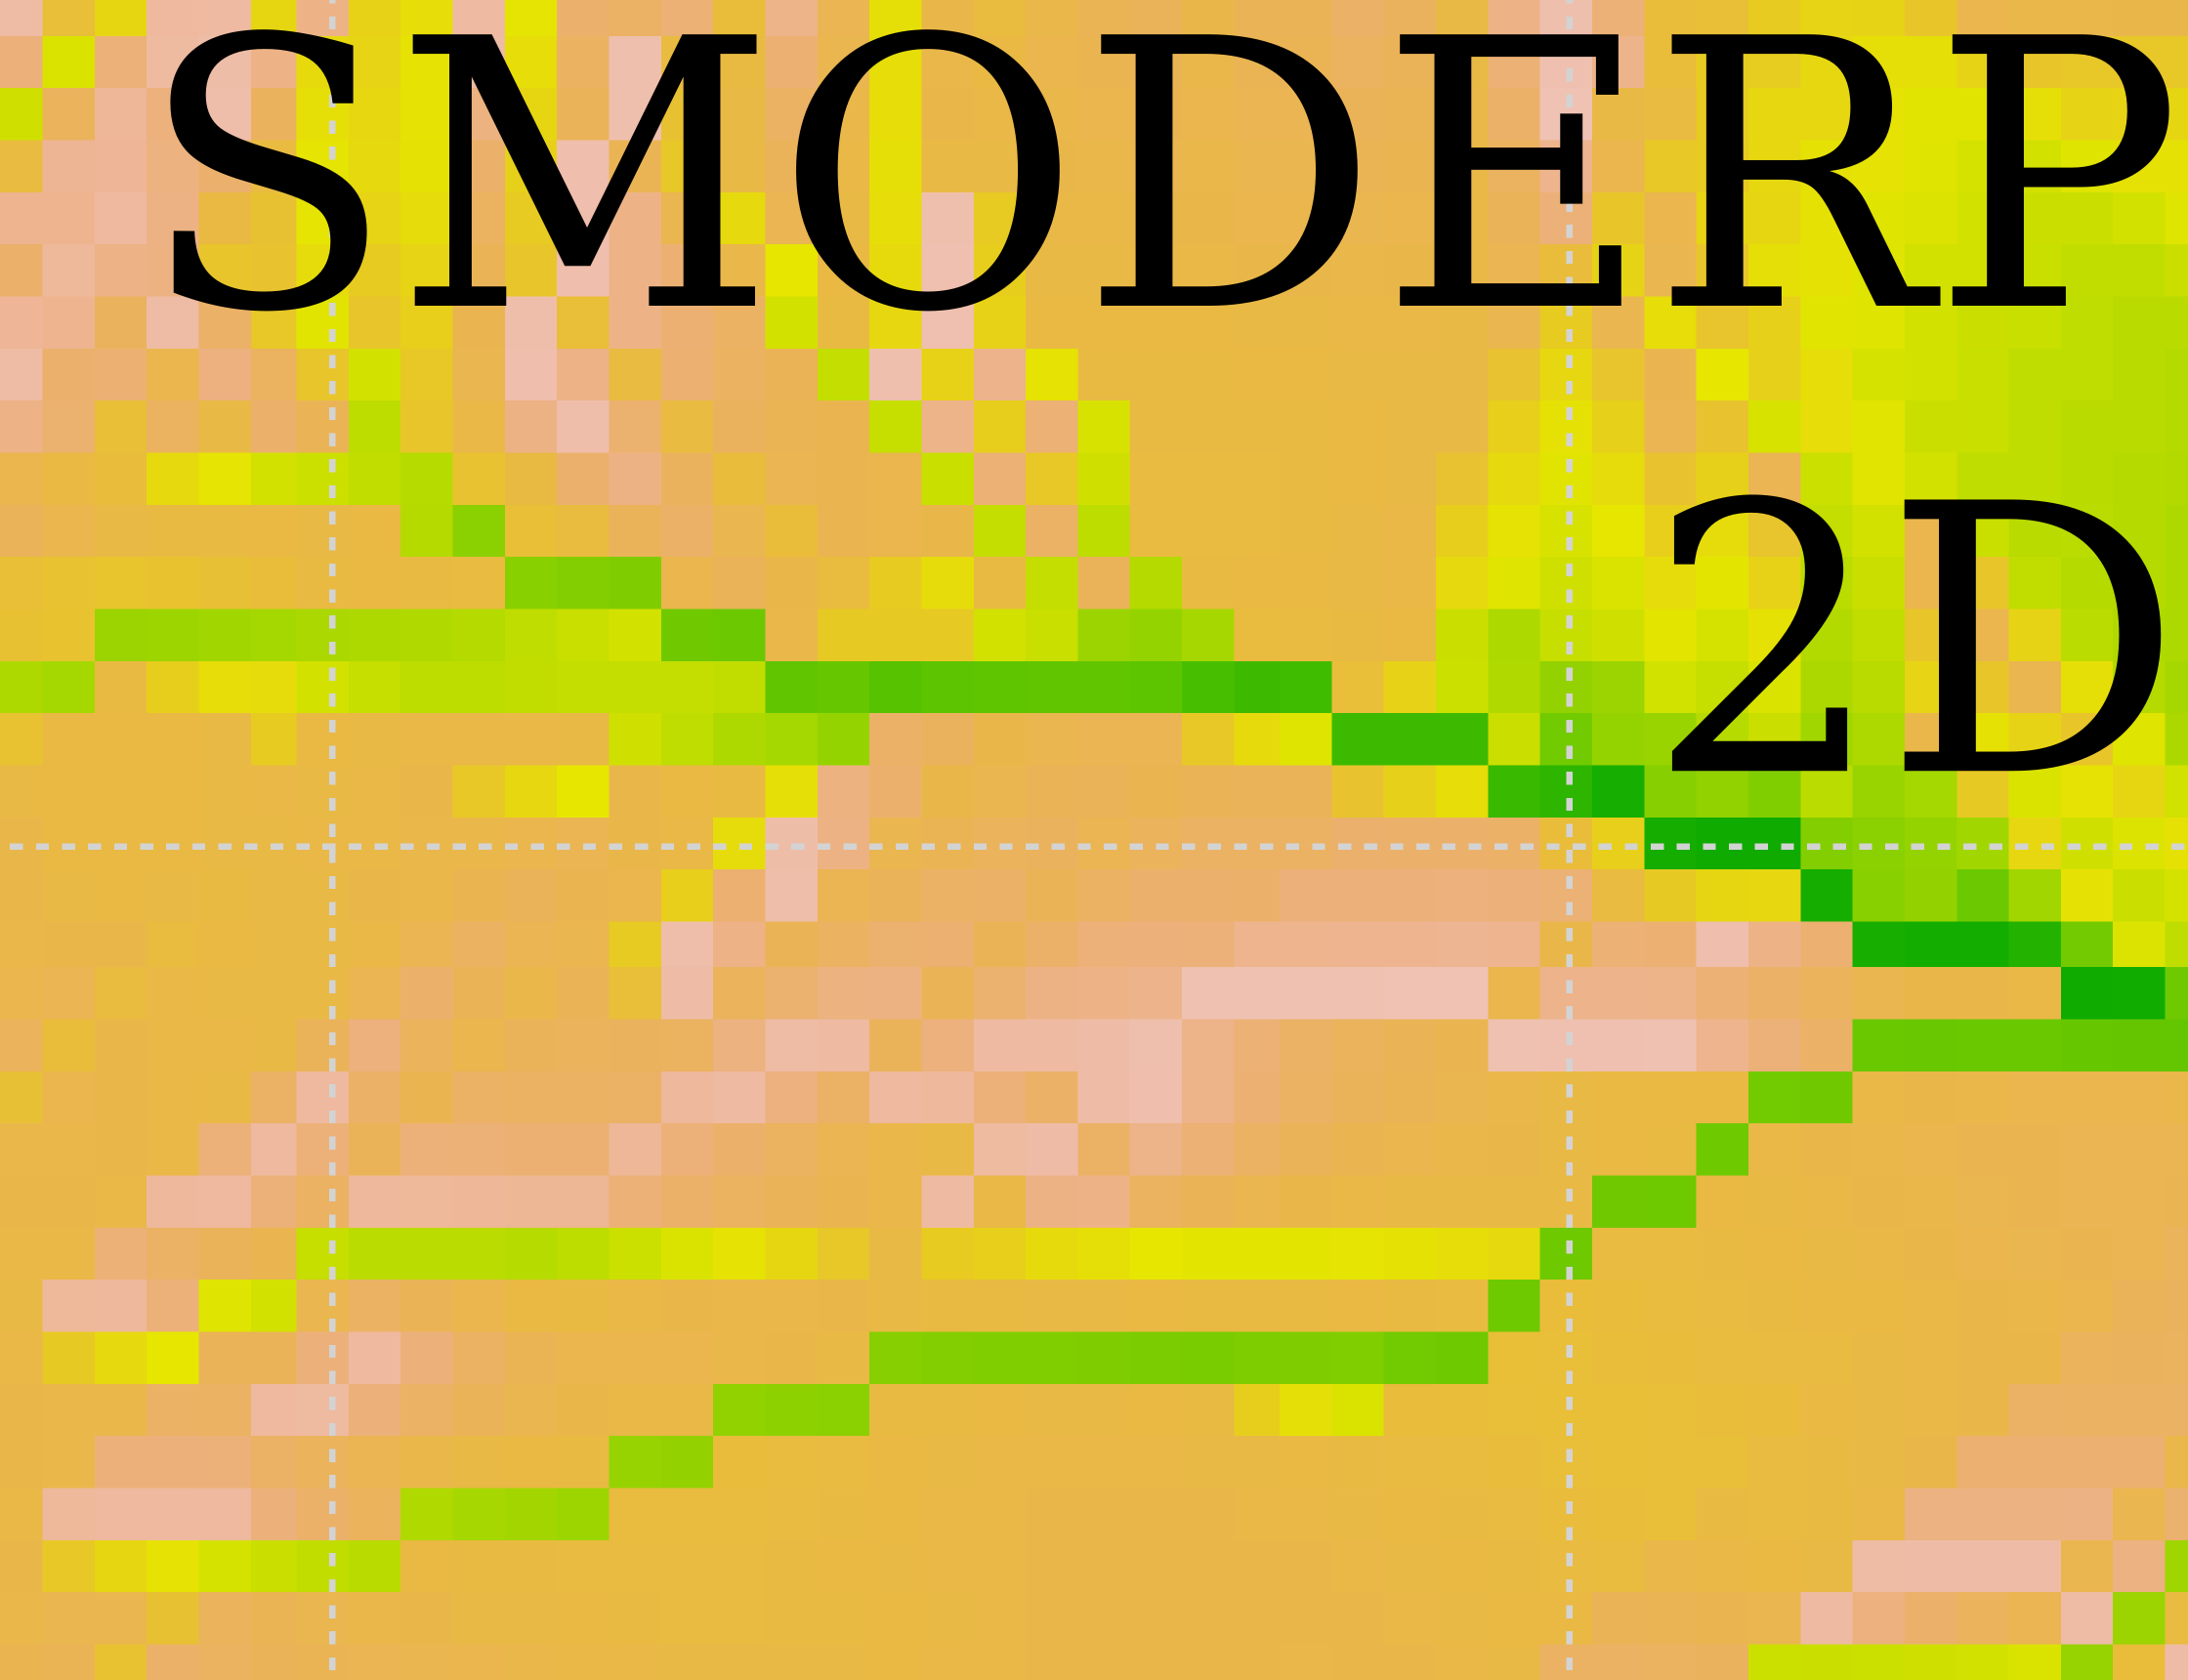
\includegraphics[width=10cm]{./img/logo.png}
% 	\plogo % Publisher logo
        
	
	\vspace{0.3\baselineskip} % Whitespace under the publisher logo
	
	2017 % Publication year
	
	{\large publisher} % Publisher

\end{titlepage}

%----------------------------------------------------------------------------------------






  \newpage
  \pagenumbering{roman}\setcounter{page}{1} % obsah a seznamy skratek, obrazku a tabulek rimska cislice od i
  \tableofcontents\addcontentsline{toc}{section}{Obsah}


  \newpage
  \section*{Seznam zkratek}\addcontentsline{toc}{subsection}{Seznam zkratek}
  \begin{multicols}{2}
  \begin{acronym}
\setlength{\parskip}{0ex}
\setlength{\itemsep}{1ex}

\acro{a}[$a$]{parametr MKWA}
\acro{A}[$A$]{průtočná plocha  [$m^{2}$]}
\acro{b}[$b$]{parametr MKWA}
\acro{bhs}[$b$]{šířka dna příčného profilu hydrografické sítě [$m$]}
\acro{brill}[$b_{rill}$]{šířka rýhy [$m$]}
\acro{BrutoSR}[$B_{\Delta t}$]{srážka [$m$]}

\acro{CFL}[$CFL$]{Courant-Friedrich-Lewy podmínka}


\acro{D8}[$D8$]{jednosměrný odtokový algoritmus}

\acro{dT}[$\Delta t$]{časový krok [$s$]}
\acro{dTmax}[$\Delta t_{max}$]{maximální časový krok [$s$]}
\acro{dTmult}[$\Delta t_{mult}$]{multiplikátor časový krok [$-$]}
\acro{dX}[$\Delta x$]{prostorový krok [$m$]}
\acro{dS}[$\frac{\mathrm{d}S}{\mathrm{d}t}$]{změna zásoby [$m^3/s$]}

\acro{ES}[$ES$]{efektivní srážka [$m^3/s$]}
\acro{es}[$es$]{intenzita efektivní srážky [$m/s$]}
\acro{effVrst}[$l_{eff}$]{efektivní vrstevnice [$m$]}

\acro{hcrit}[$h_{crit}$]{kritická hloubka [$m$]}
\acro{hrill}[$h^{rill}$]{hloubka rýhy [$m$]}
\acro{hsur}[$h^{sur}$]{výška hladiny na povrchu [$m$]}
\acro{HyVod}[$k$]{nasycená hydraulická vodivost [$m s^{-1}$]}
\acro{i}[$i$]{řešený element}

\acro{Inf}[$Inf$]{infiltrované množství [$m^3/s$]}
\acro{inf}[$inf$]{intenzita infiltrace [$m/s$]}

% \acro{VItot}[$\dot{I_{tot}}$]{celkový přítok [$m^3/s$]}
\acro{Itot}[$I_{tot}$]{celkový přítok za čas [$m^3/s$]}

\acro{I}[$I$]{sklon [$-$]}

\acro{K}[$K$]{součinitel šířky (pro plošný odtok K = 1)}
\acro{Ki}[$K_i$]{nasycená hydraulická vodivost v buňce $i$ [$m/s$]}

\acro{Lai}[$I_{LAI}$]{poměrná plocha listová}
\acro{lrill}[$l_{rill}$]{délka rýhy [$m$]}
\acro{MKWA}[$MKWA$]{modifikovaná rovnice kinematické vlny}

\acro{mfda}[$mfda$]{vícesměrný odtokový algoritmus}
\acro{m}[$m$]{poměr sklonu svahů (pro obdélník je roven nule)}

\acro{n}[$n$]{mannigův součinitel drsnosti}
\acro{NetoSR}[$I_{N}$]{efektivní srážka}

\acro{PS}[$PS$]{potenciální srážka [$m$]}

% \acro{VOtot}[$\dot{O_{tot}}$]{odtokové množství [$m^{3}$]}
\acro{Otot}[$O_{tot}$]{odtokové množství za čas [$m^{3}/s$]}
% \acro{VOin}[$\dot{O^{in}}$]{objem přítoku ze sousední buňky [$m^{3}$]}
\acro{Oin}[$O^{in}$]{přítok ze sousední buňky  za čas [$m^{3}/s$]}
\acro{oin}[$o^{in}$]{výška vtoku za čas [$m/s$]}
\acro{oinrill}[$o^{in}_{rill}$]{výška vtoku v rýze za čas [$m/s$]}
% \acro{VOout}[$\dot{O^{out}}$]{objem odtoku z buňky [$m^{3}$]}
\acro{Oout}[$O^{out}$]{odtok z buňky  za čas [$m^{3}/s$]}
\acro{oout}[$o^{out}$]{výška odtoku z buňky  za čas [$m/s$]}
\acro{ooutrill}[$o^{out}_{rill}$]{výška odtoku v rýze za čas [$m/s$]}


\acro{Q365}[$Q365$]{základní průtok [$m^3/s$]}

\acro{Orill}[$O_{rill}$]{objem odtoku - rýhový odtok [$m^{3}$]}
\acro{Osur}[$O_{sur}$]{objem odtoku - plošný odtok [$m^{3}$]}
\acro{O}[$O$]{omočený obvod [$m$]}
\acro{PotI}[$I_{POT}$]{potencionální intercepce}
\acro{q}[$q$]{průtok [$m^{3}{s}^{-1}$]}
\acro{qrill}[$q_{rill}$]{průtok v rýhách [$m^{3}/s$]}
\acro{qsur}[$q_{sur}$]{specifický plošný průtok [$m^{2}/s$]}
% \acro{Qtot}[$q_{t}$]{celkový odtok}

\acro{qstream}[$q_{stream}$]{průtok v otevřeném korytě [$m^{3}/s$]}

\acro{Rrill}[$R_{rill}$]{hydraulický poloměr v rýze [m]}
\acro{Rstream}[$R_{stream}$]{hydraulický poloměr v otevřeném korytě [m]}

\acro{ret}[$ret$]{povrchová retence [m]}

\acro{R2}[$R^2$]{koeficient determinace}
\acro{ro}[$\rho$]{hustota [$kg/m^{3}$]}
\acro{rratio}[$rill_{ratio}$]{parametr tvaru rýhy [-]}
\acro{ratio}[$ratio$]{celočíselný faktor dělící časový krok při výpočtu rýhového odtoku}
\acro{slope}[$i_{0}$]{sklon[-]}
\acro{Sorb}[$S$]{sorptivita půdy [$m \sqrt{s}$]}
\acro{Sorbi}[$S_{i}$]{sorptivita půdy  v buňce $i$  [$m \sqrt{s}$]}
\acro{S}[$S$]{sorptivita půdy [$m \sqrt{s}$]}
\acro{t}[$t$]{časový krok[$s$]}
\acro{tausur}[$\tau_{sur}$]{tečné napětí [$Pa$]}
\acro{taucrit}[$\tau_{crit}$]{kritické tečné napětí [$Pa$]}

\acro{Vout}[$V_{out}$]{objem objem odtelkého [$m^{3}$]}

\acro{Vcrit}[$V_{crit}$]{objem vody do kritické hladiny [$m^{3}$]}
\acro{vrill}[$v_{rill}$]{rychlost proudění - rýhový odtok [$m/s$]}
\acro{Vrill}[$V_{rill}$]{objem vody v rýze v daném elementu [$m^{3}$]}
\acro{vsur}[$v_{sur}$]{rychlost proudění - plošný odtok [$m/s$]}
\acro{Vtot}[$V_{tot}$]{celkový objem vody v elementu [$m^{3}$]}
\acro{vstream}[$v_{stream}$]{rychlost proudění v úseku hydrografické sítě [$m/s$]}
\acro{vcrit}[$v_{crit}$]{kritická nevymílací rychlost [$m/s$]}
\acro{X}[$X$]{parametr MKWA}
\acro{Y}[$Y$]{parametr MKWA}
\acro{GIS}[$GIS$]{geografické informační systémy}
\acro{g}[$g$]{gravitační zrychlení [$m/s^{2}$]}

\acro{ij}[$i, j$]{souřadnice elementu - buňky}
\acro{MD8}[$MD8$]{Multiple Flow Direction Algorithm}

\acro{bunka}[$P$]{plocha buňky [$m^2$]}



\end{acronym}
%1to je \ac{MLS}
%2to je \acl{MLS}
%3to je \acs{MLS} 
  \end{multicols}

  %\listoffigures\addcontentsline{toc}{subsection}{Seznam obrázků}
  %\listoftables\addcontentsline{toc}{subsection}{Seznam tabulek}


  \newpage
  \pagenumbering{arabic}\setcounter{page}{1}% od uvodu do konce arabske cislice od 1
  \part*{Úvod}

  %!TEX ROOT = ../main.tex


%\clearpage
%\newpage\null\thispagestyle{empty}\newpage

Dostává se Vám do ruky uživatelský manuál modelu \smod. Celý názvem modelu je: Simulační Model Povrchového Odtoku a Erozního Procesu. Tento model lze využít pro výpočet hydrologicko erozních procesů na jednotlivých pozemcích nebo na malých povodích. Výstupy z modelu jsou primárně určeny pro stanovení odtokových poměrů v ploše povodí a parametrů opatření pro snížení odtoku z povodí a erozního ohrožení zemědělské půdy. Model lze využít při navrhování komplexnějších soustav sběrných a odváděcích prvků nebo suchých nádrží a polderů. Jeho využití předpokládají jak současné metodiky, tak i technické normy a doporučené standardy.
Z hlediska kategorizace modelu se jedná o fyzikálně založený plně distribuovaný dvourozměrný model epizodní model. Nově zavedené prostorové řešení (2D), které nahradilo dřívější profilovou verzi modelu, umožňuje komplexní řešení a náhled na celou řešenou lokalitu. Dvourozměrné řešení je z hlediska vstupních dat a vnitřních procesů složitější, nicméně benefity distribuovaného řešení převažují. Dostupnost vstupních dat v podrobném rozlišení se zlepšuje, stejně tak jako se zvyšuje výpočetní kapacita výpočetní techniky.
Vývoj modelu je podporován z veřejných prostředků a podílejí se na něm studenti a zaměstnanci Katedry hydromeliorací a krajinného inženýrství Fakulty stavební ČVUT v Praze
Pro snazší orientaci je manuál je rozdělen na tři základní části. V první části jsou uvedeny výpočtové vztahy a popis jednotlivých zvolených procesů. Druhá část je věnována vstupním a výstupním datům a je zde stručně popsán tok programu. V třetí části jsou ukázány výsledky při řečení konkrétní lokality.
Případné aktualizace modelu, vzorová data, ukázky využití a další informace jsou pak průběžně poskytovány na stránkách  modelu
(\href{http://storm.fsv.cvut.cz/cinnost-katedry/volne-stazitelne-vysledky/smoderp/?lang=cz}{storm.fsv.cvut.cz/cinnost-katedry/volne-stazitelne-vysledky/smoderp/}).
  %%%%% %!TEX ROOT = ../main.tex

%!TEX ROOT = ../../main.tex
Water erosion is one of the most widespread forms of soil degradation. Reducing the erosion is one of many challenges worldwide and Europe \citep{LieveVan-Camp2004} or \citep{Boardman2006}. In particular, sediment transport from arable land into surface waters (streams, rivers, reservoirs) is one of the major problems of water management. Measuring and consequence modeling of the surface process are a necessary tool for the protection of the soil.

Two major surface processes influenced erosion (i) sheet flow with sheet erosion  and (ii) rill processes. Sheet flow energy is less than kinetic energy of the raindrops in sheet erosion \citep{Bryan2000}. Rate of erosion are influenced by vegetation cover that reduced impact of the rain energy. In the other hand rill erosion is generated by a concentrated flow and this process are more closely to stream processes  \cite{Gimenez2008, Govers2007}.

It is difficult to describe annual rate of soil erosion in the watershed over spatial and time scales. Long-term measurements and sufficient data base needed in order to investigate the response of erosion rates. Only abnormally high rainfall or an extreme event can produce main part of soil damage. Spatial scale of measuring are crutial as well. Many studies that focused to scaling (temporal and spatial) are published. For example \cite{Chaplot2012} deal with comparison of runoff and soil loss across the scales. In other studies \cite{Cerdan2002, Auerswald2009, BauerSGEM} the effect of the scales to erosion is evident.  

In a few available studies, the sediment yield from a hill slope or a catchment is likely to be less than the total sediment mobilised within it and estimated from plots  \cite{Walling1983}. Due to sedimentation, only a relatively small proportion of the detached and transported soil material reaches  the catchment outlet \cite{Beven2005, Verstraeten2001}.  Additional measurements and observations in different spatial scales in one place is  still required.

\newline
Long therm field measuring have uncertainty in feather. Rainfall simulation is one of the way that make possible to measured in controlled condition. %!TEX ROOT = ../main.tex
Rainfall simulation experiments are widely used as a standard method to study various flow and transport processes induced by rainfall. They have been used on different slopes, scales, soils and vegetation cover  \cite{Otero2011, Davidova2016}, etc. Surface runoff rate and sediment yield are standard variables observed in experiments oriented on soil erosion research with use of rainfall simulators. The review of simulators used across Europe provides (Iserloh, 2013). Due to the nature of the device the small simulators with watered area around 1 m2 are more frequent. Larger simulators can be found as well, as described for example in \cite{Sanguesa2010}, \cite{Strauss2000} \cite{Marques2007},  \citep{EGUDS}.
\newline
Long-therm measuring and rainfall simulations are essential for a consequent mathematical modeling. %!TEX ROOT = ../main.tex
Computer based physical models can be used for erosion prediction over a wide range of conditions. To ensure model validity, simulation results must be compared with field measurements. Models can only work when they are applied to conditions. Due A desirable model should satisfy the requirements of universal acceptability; reliability; robustness in nature; ease in use with a minimum of data; and ability to take account of changes in land use, climate and conservation practices.

Many models was created and are constantly improved over the last twenty years. The specific conditions of formation, calibration and use of each models can't lead to universally valid model. General review article about models are in \cite{Pandey2016}. These fifty selected models essentially reflects the wide range of models including classification according they characterization.

Mathematical modeling is very important for describing erosion processes and for soil conservation. Generally, there are two types of models of soil erosion and surface runoff: (i) empirical models often USLE \citep{Wischmeier1978} or RUSLE \citep{Renard1991} based and (ii) physically based models. Parameterisation of the emperical models based on measurements often at standardised field plots in accordance with the estimation of USLE factors or on datasets from rainfall simulators \citep{Davidova2016}. 
Physically based models have for their goal to create a mathematical description of  process. Hydrolgical and hydraulical equations for watter balance and moving are base of approach. The models principally describe the processes of precipitation, infiltration, evapotranspiration, surface runoff, influence of vegetation. Loading, trasportation and sedimentation processes are in interconnection with surface water processes. Interconnections of precipitation, runoff, infiltration and soil erosion have become very important topics. A wide group of the models can be represented by WEPP \citep{Laflen1997}, KINEROS \citep{Woolhiser1989}, EROSION 2D/3D \citep{Schindewolf2012a} and model SMODERP that is object of this this article.




%\clearpage
%\newpage\null\thispagestyle{empty}\newpage


  \newpage
  \part{Popis řešení}\label{cast:1}
  %!TEX ROOT = ../mainCZ.tex
%\input{./1_text/3_mat_a_met/2}

První část manuálu popisuje jednotlivé výpočetní vztahy použité v modelu \smod. Základní odvození povrchových procesů v modelu \smod vychází z rovnice kontinuity a pohybové rovnice. Pohybová rovnice je zjednodušená pomocí teorie kinematické vlny. Tímto způsobem je tok řízen mocninný vztahem, jehož parametry byly měřeny (viz  příloha~\ref{sec:priloha}). 

Jak již bylo zmíněno v úvodu, model \smod je distribuovaný epizodní hydrologicko-erozní model. Výpočet je řešen na pravidelné rastrové síti. Prostorová diskretizace modelu je řízena  rozlišením vstupního digitálního modelu terénu. V celém řešeném prostoru je po jednotlivých buňkách v každém časovém kroku provedena bilance vstupů a výstupů a následně vypočteno odteklé množství v daném časovém úseku v buňce. Formálně se jedná o řešení metodou konečných diferencí s explicitně řešenou časovou diskretizací. V bilanční rovnici jsou řešeny tři základní složky:


\begin{itemize}\itemsep 0cm
\item infiltrace do půdy \acs{Inf},
\item efektivní srážka \acs{ES},
\item přiteklé a odteklé množství \acs{Itot} a \acs{Otot}.
\end{itemize}


Odteklé množství může být dále složeno ze tří základních typů odtoku: \textbf{plošného} povrchového odtoku, \textbf{soustředěného rýhového} povrchového odtoku a odtoku dočasnou \textbf{hydrografickou sítí} (tok otevřeným korytem). V ploše povodí jsou směry odtoků odvozeny na zahladě odtokových algoritmů. V místě úseků hydrografické sítě je veškerý tok směrován touto sítí.\\
% PeKa - pokuso jsem se rozdělit povrchový odtok (plošný a rýhy dohromady), ab bylo jasnější o co jde
% 
% 
\rule{\textwidth}{0.3pt}
% % % % %	\subsubsection{Použité rovnice}
%%!TEX ROOT = ../mainCZ.tex
% 
% 
% 
%
% Plošný povrchový odtok
%
%
%
Základní odvození vztahů povrchových procesů v modelu SMODERP vychází z rovnice kontinuity a rovnice pohybové na základě kinematického principu s využitím experimentálních měření.
Jak již bylo zmíněno v úvodu, jedná se o distribuovaný epizodní hydrologicko erozní model. Výpočet je řešen na pravidelné rastrové síti elementů. Podrobnost řešení je dána rozlišením vstupního rastru. V celém řešeném prostou je po jednotlivých elementech v každém časovém kroku provedena bilance zásoby a následně vypočteno odteklého množství za daný časový krok. Obecně se jedná o tři základní složky:

\begin{itemize}
\item infiltrace do půdy\acs{Inf}
\item efektivní srážka \acs{ES}
\item odteklé množství \acs{Otot}
\end{itemize}

Proudění povrchové vody a množství odtoku je pak podle řešeno třemi odlišnými typy odtoku:
\begin{itemize}
\item plošný odtok
\item soustředěný odtok v rýhách
\item výpočet odtoku v hydrografické síti
\end{itemize}

V ploše povodí jsou směry odtoků resp. přítoků dány funkcí směru odtoku. V místě vodních toků je pak veškerý tok směrován dále vodním tokem.


\subsubsection{Plošný povrchový odtok} 

% 
% 
% 
% 
Základním vztahem řešení v elementu je bilance plošného odtoku.
\begin{equation}
\acs{dS} = \acs{Itot} - \acs{Otot},
\label{eq:bilobecne}
\end{equation}
% 
% 
% 
% kde se aktuální změna  zásoby $S$ rovná rozdílu sumy aktuálních přítoků  \acs{Itot} a sumy aktuálních odtoků \acs{Otot}.
\begin{tabular}{rrl}
  kde \jj{dS}{,}
      \jj{Itot}{,}
      \jj{Otot}{.}
\end{tabular}




Podle složek povrchového odtoku lze \acs{Itot} a \acs{Otot} rovnici~\ref{eq:bilobecne}  rozepsat takto podle složek povrchového odtoku použitých v modelu SMODERP 




$$
  \acs{Itot} = \acs{ES} + \acs{Oin},
$$
$$
  \acs{Otot} = \acs{Inf} + \acs{Oout},
$$
% 
% kde \acs{Oin} je přítok ze sousední výpočetní buňky (buněk) a \acs{Oout} je odtok z dané buňky. 
\begin{tabular}{rrl}
  kde \jj{Oin}{,}
      \jj{Oout}{,}
      \jj{ES}{,}      
      \jj{Inf}{.}
\end{tabular}


Bilanční rovnici pro každou buňku $i$ v čase $t$ lze rozepsat jako




\begin{equation} 
\frac{\mathrm{d}S}{\mathrm{d}t} = \acs{ES}_{i,t} + \sum_j^m \acs{Oin}_{j,t-1} - \acs{Inf}_{i,t} - \acs{Oout}_{i,t-1},
\label{eq:bilancnirceV}
\end{equation}
% 
% 
% 
% kde $m$ jsou buňky, odkud vtéká voda do buňky $i$. 
\begin{tabular}{rrl}
  kde & $m$ & jsou buňky, odkud vtéká voda do buňky $i$. 
\end{tabular}


Toto $m$ se liší podle použitého odtokového algoritmu jednosměrného \acs{D8} nebo vícesměrného \acs{mfda} ({\it multi-flow direction algorithm}). Objem srážky \acs{ES} a infiltrované množství \acs{Inf} lze určit přímo při výpočtu časového kroku $t$. Přiteklé a odteklé množství vody \acs{Oin} a \acs{Oout} z časového kroku $t-1$ (což odpovídá explicitnímu řešení časové derivace). 




Při samotném řešení se v modelu SMODERP operuje s veličinami ve výškových jednotkách. Pokud celou rovnici~\ref{eq:bilancnirceV} podělíme velkostí buňky \acs{bunka} a vyjádříme časovou derivaci jako diferenci ($\frac{\mathrm{d}\acs{hsur}_{i,t}}{\mathrm{d}t} \approx \frac{\acs{hsur}_{i,t} - \acs{hsur}_{i,t-1}}{\acs{dT}}$), vypadá rovnice~\ref{eq:bilancnirceV} následovně:




\begin{equation} 
\acs{hsur}_{i,t} = \acs{hsur}_{i,t-1} + \acs{dT}\left(\acs{es}_{i,t} + \sum_j^m \acs{oin}_{j,t-1} - \acs{inf}_{i,t} - \acs{oout}_{i,t-1}\right),
\label{eq:bilancnirce}
\end{equation}
% 
% 
% 
% 
% kde \acs{hsur} je výška hladiny na povrchu, \acs{es} je intenzita srářky, \acs{inf} je intenzita infiltrace, \acs{oin}(\acs{oout}) odteklá (přiteklá) výška za čas. 
\begin{tabular}{rrl}
  kde \jj{hsur}{,}
      \jj{es}{,}
      \jj{inf}{,}
      \jj{oin}{,}
      \jj{oout}{.}
\end{tabular}
% 
% 
\\ V následujícím textu jsou popsány jednotlivé členy za pravé straně rovnice~\ref{eq:bilancnirce}.


% 
% 
% 
% 
% 
% 
% Efektivní srážka \acs{ES}
% 
% 
% 
% 
% 
% 
% 
\paragraph{Efektivní srážka \acs{es}} 

Srážka je příčinou celého erozního procesu. Vzhledem k tomu, že se jedná o epizodní model je srážka zadávána v podobě konkrétní nebo návrhové srážky, která začíná s prvním časovým krokem výpočtu. Model počítá s vlivem intercepce, tedy že určitá část srážky bude zachycena rostlinami díky potenciální intercepci \acs{PotI}. Míra zachycení v každém výpočtovém čase je definována  pomocí poměrné plochy listové \acs{Lai} například \cite{Nevim}.

Označme množství srážky který dopadá na povrch půdy i plodiny během \acs{dT} potenciální srážkou \acs{PS}. Část \acs{PS}, která zůstane v časovém kroku na rostlinách se dá vyjádřit jako násobek srážky \acs{PS} a \acs{Lai},
$$
\acs{PS}\ I_{LAI}
$$
% 
Z tohoto vztahu vyplývá, že množství které propadne povrchem listů je 
$$
\acs{PS}(1 - I_{LAI}).
$$

V modelu je rovněž zahrnuta intercepční kapacita \acs{PotI}, která se plní na začátku běhu modelu. Výsledná intenzita efektivní srážky v čase $t$ je par určena jako
$$
 \acs{es}_t = MAX(0;\sum_{\bar{t} = t_{init}}^{t}\left(\acs{PS}_{\bar{t}}(1 - I_{LAI})\right)-\acs{PotI}))/\acs{dT},
$$
% kde suma $\sum_{\bar{t} = t_{init}}^{t}$ vyjadřuje množství srážky které propadlo povrchem listů plodiny od počátečního času $t_{init}$ do času $t$.
\begin{tabular}{rrl}
  kde \jj{PS}{,}
      \jj{Lai}{,}
      \jj{PotI}{\ a}
      & $\sum_{\bar{t} = t_{init}}^{t}$ & vyjadřuje množství srážky které propadlo \\
      && povrchem listů plodiny od počátečního času $t_{init}$ do času $t$.
\end{tabular}



% 
% 
% 
% 
% 
% 
% 
% 
% 
% 
\paragraph{Intenzita infiltrace \acs{inf}}

V modelu je použita infiltrace podle Philipa \citep{philip1957} v~následujícím tvaru (pro příslušnou buňku $i$):
\begin{eqnarray} \label{eq:phillip}
\acs{inf} = \frac{1}{2}\acs{Sorb}t^{-1/2}+\acs{Ki}.
\end{eqnarray}
% 
% 
\begin{tabular}{rrl}
  kde \jj{inf}{,}
      \jj{Sorb}{\ a}
      \jj{Ki}{.}
\end{tabular}




Philipova rovnice byla zvolena především z důvodu relativně malého počtu nutných vstupních parametrů. tato zjednodušená rovnice má dva hlavní členy nasycenou hydraulickou vodivost \acs{K} a sorbtivitu \acs{Sorb}. Autoři modelu si byli vědomi omezení použití Philipovy rovnice vyplývající z podmínek, za kterých byla odvozena.  Možné odchylky způsobené volbou této rovnice odpovídají odchylkám v heterogenitě půdy a kvalitě ostatních vstupů, na jejichž základě model pracuje. Čas $t$ ve vztahu~\ref{eq:phillip} je čas od začátku srážky, který by měl být v epizodním modelu totožný s počátečním časem výpočtu. Tato nezbytná podmínka by měla být brána v potaz při přípravě vstupních dat. 
% 
% 
% 
% 
% 
% 
% 
% 
% 
% 
% 
\paragraph{Plošný odtok  \acs{oin}, \acs{oout}} \label{rce_odtok}
Rovnice plošného odtoku vychází z kinematického přístupu k řešení pohybové rovnice,
% 
% 
% 
$$
  \acs{qsur} = \acs{a}\acs{hsur}^{\acs{b}},
$$
% 
% 
% 
\begin{tabular}{rrl}
  kde \jj{qsur}{,}
      \jj{a}{\ ($a = \acs{X}\acs{I}^{\acs{Y}}$)\ a}
      \jj{b}{.}
\end{tabular}




Parametry \acs{a} a \acs{b} respektive \acs{X} a \acs{Y} jsou odvozeny na základě měření, viz kapitola \ref{Exp_mer}. Z vyhodnocení vyplývá, že parametr b je závislý pouze na půdním druhu. Parametr a je závislý nejen na půdním druhu, ale také na sklonu svahu. Odteklá resp. přitelká výška je pak dopočítána jako



$$
   \acs{oout} (resp.\ \acs{oin}) = \frac{\acs{dX}}{\acs{bunka}}\acs{qsur}
$$
%
% 
\begin{tabular}{rrl}
  kde \jj{dX}{\ a}
      \jj{bunka}{.}
\end{tabular}

% $$
% q_{sur} [m^{3}/s] = Ah_{sur}^{b} \Rightarrow \frac {1}{n} a h_{sur}^{X} i_{0}^{Y}
% $$

\textbf{ověřit sklon v\%}

% 
% 
% 
% 
% 
% 
% 
% 
% 
% 
% 
% 

\paragraph{Odvozené veličiny}

Z vypočteného průtoku, velikosti řešeného elementu a délky časového lze dopočítat objem odtoku
$$
  \acs{Vout} = \acs{dT}\acs{qsur},
$$
% 
% 
% 
% 
\begin{tabular}{rrl}
  kde \jj{Vout}{.}
\end{tabular}




Pro posouzení erozní ohroženosti a pro výpočet vzniku rýh je v každém elementu vypočítávána rychlost a tečné napětí. Za předpokladu, že se jedná a proudění vody o malé hloubce, lze rychlost proudění odvodit ze specifického průtoku a výšky hladiny:
% 
% 
% 
% 
% 
\begin{equation}
  \acs{vsur} =  \frac{\acs{qsur}}{\acs{hsur}},
  \label{eg:v}
\end{equation}
% 
% 
% 
\begin{tabular}{rrl}
  kde \jj{vsur}{.}
\end{tabular}




Tečné napětí dále využívané v modelu pak uvažuje výpočet tak, jak jej uvádí například \citep{Schwab1993}
% 
% 
% 
\begin{equation}
\acs{tau} = \acs{ro} \acs{g} \acs{hsur} \acs{I}\acs{K} \label{eg:tau},
\end{equation}
% 
% 
% 
\begin{tabular}{rrl}
  kde \jj{tau}{,}
      \jj{ro}{,}
      \jj{g}{,}
      \jj{I}{\ a}
      \jj{K}{.}
\end{tabular}



Vypočítaná rychlost a tečné napětí jsou v případě posuzování erozní ohroženosti porovnávány s limitními hodnotami krajních nevymílajících rychlostí a tečnéch napětí pro jednotlivé půdní druhy v závislosti na druhu vegetace \citep{DyrovaE.1984} a jsou uvedeny v tabulce 
\ref{tabulkaDyrova}. % tabulka neni 
V literatuře se setkáme i s odlišnými hodnotami. Například M. A. Velikanov stanovil krajní nevymílající rychlost pro půdy 0,24 $m/s$  \citep{CabikJ.1963}, což je hodnota nižší, než kterou stanovila E. Dýrová.


% 
% 
% 
% 
% 
% 
% 
% 
% 
% 
% 
\subsubsection{Soustředěný odtok v rýhách} \label{sec:soustredenyodtok}

Výpočet soustředěného odtoku v rýhách implementovaný do modelu SMODERP vychází z několika předpokladů:
\begin{enumerate}
  \item Zavedení stejných zjednodušujících předpokladů výpočtu proudění obdobně jako v~případě výpočtu plošného odtoku, přesto že se nejednáo výpočet proudění o zanedbatelně malé hloubce. Předpokladem je, že se v jednotlivých elemetech v relativně malých časových krocích jedná o rovnoměrné ustálené proudění. Při rovnoměrném proudění se předpokládá sklon dna \acs{I} rovný sklonu hladiny vody v rýze a shodná drsnost v celé délce elementu. Průtok v rýze je vyjádřen použitím Chézyho rovnice v mannigově tvaru:
  \begin{equation}
    \acs{qrill} = \acs{vrill} \acs{A} = \acs{A} \frac{1}{\acs{n}} \acs{Rrill}^{2/3} \acs{I}^{1/2}  ,
    \label{eq:qrill}
  \end{equation}
  \begin{tabular}{rrl}
    kde \jj{qrill}{,}
        \jj{vrill}{,}
        \jj{A}{,}
        \jj{n}{\ a}
        \jj{Rrill}{.}
  \end{tabular}

  
  
  \item Soustředěný odtok vniká v elementech, kde dojde k překročení kritické hladiny \acs{hcrit}, která je spočtena pro každý element na základě  hodnot kritického tečného napětí \ref{eg:tau} nebo rychlostí \ref{eg:v}. Objem vzniklé rýhy odpovídá nadkritickému množství vody \acs{Vrill}.
  $$
  \acs{Vrill}= \acs{Vtot} - \acs{Vcrit} = MAX(0;\acs{hsur} - \acs{hcrit}) \acs{bunka}
  $$
  \begin{tabular}{rrl}
    kde \jj{Vrill}{,}
        \jj{Vtot}{,}
        \jj{Vcrit}{\ a}
        \jj{hcrit}{.}
  \end{tabular}
  

  \item Další z důležitých zjednodušení je tvar příčného profilu rýhy, který je v modelu reprezentován obdélníkem, s pevným poměrem stran \acs{rratio}=výška/šířka rýhy. Velikost rýhy se zvětšuje pokud je nadkritické množství \acs{Vrill} větší než objem samotné rýhy. Pak se výška rýhy rovná výšce vodní hladiny v rýze (vlevo na obrázku~\ref{fig:rill_schema}). Pokud začne být nadkritické množství \acs{Vrill} menší než je velikost rýhy, začne se rýha prázdnit, velkost rýhy však zůstává konstantní (vpravo na obrázku~\ref{fig:rill_schema}). Hydraulický poloměr rýhy lze určit podle následujícího vztahu
%   
% 
% 
%   Rozměry rýhy nejsou známy, protože rozměr rýhy \acs{hrill}, \acs{brill} se dynamicky mění v závislosti na množství vody během simulace. 
%   
  \begin{figure}
    \centering
    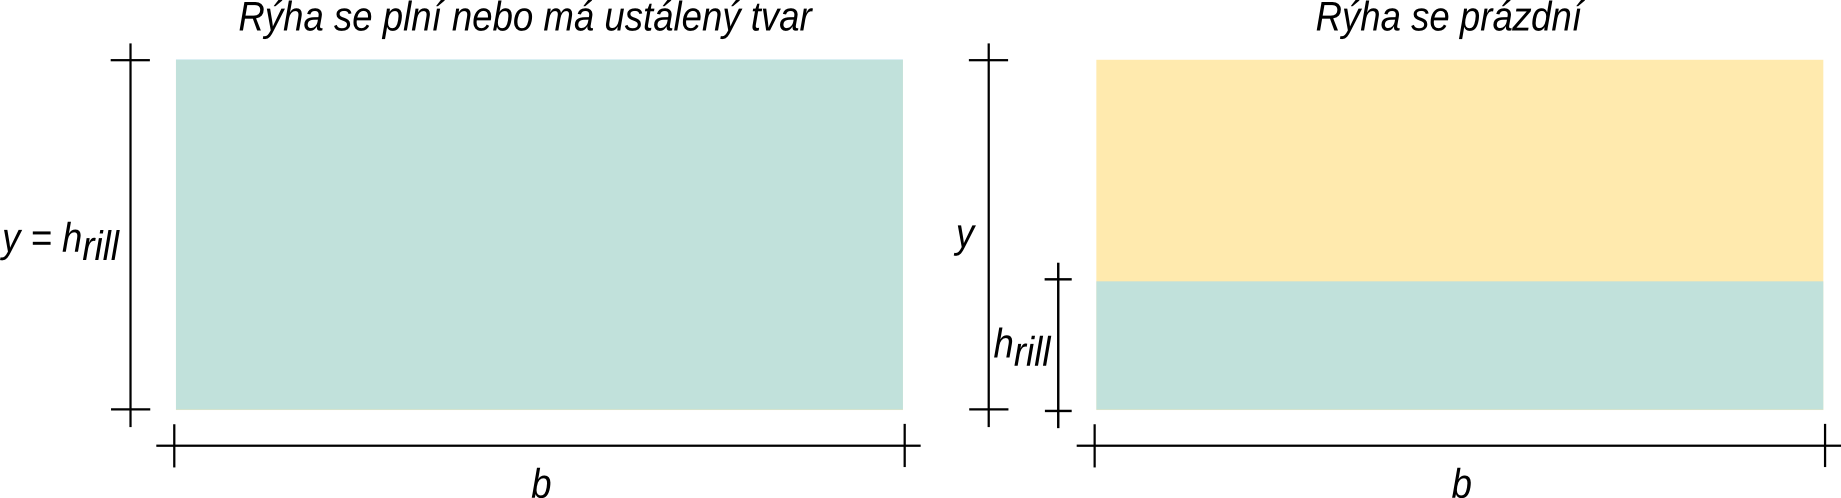
\includegraphics[width=0.9\textwidth]{./img/rill_schema.png}
    \caption{Tvar rýny a výška vodní hladiny při plnění rýny či ustálení proudění (napravo), tvar rýny při jejím prázdnění (nalevo)}
    \label{fig:rill_schema}
  \end{figure}
% 
%   
  $$ 
    \acs{Rrill} = \frac{\acs{A}}{\acs{O}} = \dfrac{\acs{hrill} \acs{brill}}{\acs{brill}+2\acs{hrill}} = \dfrac{\acs{brill}^{2} \acs{rratio}}{\acs{brill}(\acs{rratio}+2)}
  $$
  \begin{tabular}{rrl}
    kde \jj{brill}{,}
        \jj{O}{\ a}
        \jj{rratio}{.}
  \end{tabular}
  
  
%   Poměr šířky a výšky je v programu stanoven v současné době pevně, ale jako parametr, který je možné v případě potřeby změnit. Objem rýhy je stanoven podle rovnice \ref{Vrill}.

%   \item V případě poklesu objemu vody v rýze si rýha zachovává svůj maximální tvar.
\end{enumerate}


% Pro výpočet průtoku v rýze \acs{qrill} je pak možné využít Chézyho rovnici v manningově tvaru:.


\paragraph{Celková bilance}
Pokud dojde k vzniku rýh, přičtou se do celkové bilance~\ref{eq:bilancnirce} další dva členy vyjadřující přítok a odtok v rýhách. Rovnice~\ref{eq:bilancnirce} vypadá následovně

\begin{equation} 
\acs{hsur}_{i,t} = \acs{hsur}_{i,t-1} + \acs{dT}\left(\acs{es}_{i,t} + \sum_j^m \acs{oin}_{j,t-1} - \acs{inf}_{i,t} - \acs{oout}_{i,t-1}  + \sum_k^n \acs{oinrill}_{k,t-1} - \acs{ooutrill}_{i,t-1} \right),
\label{eq:bilancnircerill}
\end{equation}
  \begin{tabular}{rrl}
    kde \jj{oinrill}{\ a}
        \jj{ooutrill}{.}
        & $n$ & jsou buňky, odkud vtéká voda z rýh do buňky $i$.
  \end{tabular}\\
 $n$ může být prázdná množina pokud není překročena kritická výška nebo no může rovnat $m$ z rovnice~\ref{eq:bilancnirce} pokud je použit odtokový algoritmus \acs{D8} a na všech sousedních buňkách buňky $i$ je překročena kritická výška hladiny. 



\paragraph{Rýhový odtok \acs{oinrill}, \acs{ooutrill}}

Výška odtoku (resp. vtoku) z rýhy do dané výpočetní buňky je vypočtena za základě Chézyho rovnice~\ref{eq:qrill} takto:
$$
  \acs{oinrill} (resp.\ \acs{ooutrill}) = \frac{\acs{qrill}}{\acs{brill}\acs{lrill}}
$$
\begin{tabular}{rrl}
  kde \jj{lrill}{.}
\end{tabular}


% Množství odtoku \acs{Orill} za \acs{dT} je pak možné stanovit podle vztahu:
% \begin{eqnarray}
% O_{rill_{i,t}} [m^{3}] = \Delta t q_{sur}
% \end{eqnarray}
% 
% Tvar bilanční rovnice \ref{bilancnirce} při zavedení odtoku v rýhách pak přechází na tvar:
% \begin{eqnarray}
%   H_{i,j,t} = H_{i,j,t-1} + ES_{i,j,t} + \sum\limits_{(i,j)\in M} O_{M_{t-1}} - O_{i,j,t} - I_{nf_{i,j,t}} \label{eq:bilancenew}
% \end{eqnarray}
% \begin{equation*}
%  M = \{ (k,l) | i-1 \leq k \leq i+1 ; j-1 \leq l \leq j+1 \}
% \end{equation*}



% \textit{kde $ O_{M} $ obecně znamená jak přítok plošný, tak soustředěný v rýhách, $ O $ celkový odtok, který se podle konkrétního stavu dělí na plošný a soustředěný}





\paragraph{Poznámka nebo to dát do diskuse k článku} 
\begin{itemize}
\item Výsledný tvar blíží Maningově rovnici
\begin{eqnarray}
Q =\frac A {1}{n} R_{h}^{2/3} S^{1/2}
\end{eqnarray}
\item Přesněji pro tvar této rovnice pro plošný odtok, kdy se předpokládá proudění vody  o malé hloubce a tvar koryta je nahrazen jeho šířkou. Rovnice má pak tvar:
\begin{eqnarray}
Q =\frac {1}{n} h^{2/3} S^{1/2}
\end{eqnarray}
\item Že může být jiná rce infiltrace.
\item tvar rýhy - výzkum funkce?
\item jen jedna přímá rýha
\end{itemize}

%newb = math.sqrt(V/(rillRatio*l)) #KAvka, tohl eje divně
\subsubsection{Odtok hydrografickou sítí} \label{sec:tokyodtok}
\textbf{tohle není vůbec napsané}

kapitola nenese záměrně název vodní toky. SMODERP je zamýšlen také jako nástroj pro navrhování opatření v ploše povodí. Cílem je simulovat a navrhovat odtoky i v dočasné hydrografické síti, která je tvořena přirozeným nebo častěji umělým přerušením přirozené odtokové dráhy. Nejčastěji se jedná o příkopy a průlehy které mají odváděcí a často erozní funkci. 
Všechny prvky (síť vodních toků, přkopy, průlehy, atp.) jsou zadávány v rámci jednoho shapefile. Každý jednotlivý úsek je zadán jako konkrétní polygon (feature). Výpočetně model pracuje v rastrové síti, ale v případě, že se na daném elemetu vyskytuje tok, je přiteklá voda dále odváděna tímto tokem ve směru toku bez ohledu na směr odtoku modelu terénu.

Proudění v těchto otevřených korytech je řešeno Mannigovou rovnicí ve tvaru:

\textbf{překotrovat rci}
\begin{equation}
    \acs{qstream} = \acs{A} \frac{1}{\acs{n}} \acs{Rsheet}^{2/3} \acs{I}^{1/2}  ,
    \label{eq:qtok}
\end{equation}

%\begin{tabular}{stream}
 %   kde \jj{qstream}{,}
  %      \jj{vstream}{,}
   %     \jj{A}{,}
    %    \jj{n}{\ a}
     %   \jj{Rstream}{.}
%\end{tabular


Pro vlastní výpočet je třeba zadat typ a příčný profil daného prvku. Délka úseku je převzata z vlastností polygonu. Protože je model určen pro malá povodí jsou v modelu předpokládány pouze základní příčné profily (trojúhelník, obdélník, lichoběžník, parabola). 
Zadávání příčných profilů není přímo součástí shapefile, ale pro ulehčení jsou parametry zadávány jako samostatná tabulka. V případě, že jsou některé charakteristiky shodné, je tak možné jim přiřadit shodné atributy z tabulky.
V rámci zjednodušení výpočtu jsou zadávány profily parametricky. Zjednodušený výpočetní model neuvažuje rozlivy z koryta zpět do buněk odtoku. Jednotlivé prvky narůstají podle zvolených parametrů, tak aby veškerá voda zůstala v korytě.
přehled parametrů je uveden v následující tabulce

\textbf{vlžit tabuklu peka}

cislo	smoderp	tvar	b	m	drsnost	Q365	pozn
0	0	1.0	0.3	1.0	0.03	0.0	default
1	obdelnik1	0.0	0.2	0.0	0.035	0.0
2	lichobeznik1	1.0	0.2	2.0	0.035	0.0
3	trojuhelnik1	2.0	0	2.0	0.03	0.0
4	parabola1	3	0.7	0.0	0.03	0.0	b..sirkahladina




kde:
\begin{itemize}
\item \textbf{b} - šířka profilu ve dně (u trojúhelníku se rovná nule)
\item \textbf{m} - poměr sklonu svahů (pro obdélník je roven nule)
\item \textbf{drsnost} - Maninngova drsnost v daném korytě.
\item \textbf{Q365} - základní odtok. V případě dočasných prvků jako jsou příkopy je tato hodnota rovna nule, v případě vodních toků se jedná o základní odtok.-
\item \textbf{poznámky} - jedná se o volitelnou položku, do výpočtu se nijak nepropaguje
\end{itemize}

Tímto způsobem jsou zadávány
\textbf{sem dát obrázek těch profilů}


\textbf{doplnit text jak probíhá vlastní výpočet} - tzn jak na sebe navazují jednotivé úseky . a dát semka asi i nějaké  obrázky, jak to funguje. Je to v nějaké DP tuším (to najdu PK)










  \newpage
  \part{Použití modelu}\label{cast:2}
  Model SMODERP je napsán v programovacím jazyce Python. Příprava dat a samotný výpočet v časové smyčce jsou od sebe oddělny. Příprava dat využívá v současné době nástroje z knihoven ArcGIS, což byl jeden z primárních důvodů volby  programovacího jazyka Python, který je pro prostředí ArcGIS nativním skriptovacím jazykem. Proces samotného výpočtu již využívá pouze standardní knihovny Python, jako je knihovna \texttt{numpy}, nebo \texttt{math}, atd. Následující text je rozdělen do tří částí, které popisují vstupní data (kapitola~\ref{kap:vstupy}), tok programu (kapitola~\ref{kap:tok}) a výstupy z modelu (kapitola~\ref{kap:vystupy}).


\newpage
%%%%%%\subsubsection{Princip výpočtu} \label{kap:principvypoctu}
%%%%%%\input{./1_text/3_mat_a_met/CZsmoderp_princip}
        \setcounter{section}{0}
	
	\section{Vstupy do modelu} \label{kap:vstupy}
	%%!TEX ROOT = ../mainCZ.tex



Do modelu vstupují informace o topografii řešeného území, informace o typech půd a využití území a o jejich prostorovém rozmístění, informace o srážce případně o geometrii dočasné hydrografické síti.
Tyto data jsou zadávána ve třech formátech: rastrovém, vektorovém a textovém. Do modelu vstupují informace o topografii řešeného území, informace o typech půd a vegetaci, informace o srážce atd. Základní formát vektorových dat je formát shapefile. Tento vektorový formát byl vytvořen firmou ESRI, ale je zpracovatelný i jinými GIS softwary. Parametry modelu jsou uloženy v atributové tabulce pod specifickým názvem pole. 
% Shapefile popisuje prvky jako body, linie nebo polygony. Každý prvek má obvykle nějaký atribut, který ho popisuje jako v tomto případě jméno, či typ půdy. 
V následujícím text jsou popsány náležitosti vstupních dat. 
% 
% Model pracuje s následujícími vstupy
Přehled vstupů do modelu je ukázán v tabulce~\ref{tab:vstupy}.


% 

% 
\begin{sidewaystable}
% \begin{table}[]
\centering
\caption{Tabulka s přehledem vstulních dat modelu}
\label{tab:vstupy}
\small{
% \begin{tabular}{p{4cm}lp{2cm}p{5cm}}
\begin{tabular}{p{0.15\textwidth}lp{0.10\textwidth}p{0.25\textwidth}l}
\hline
Název                              & Typ dat                                               & Povinný / volitelný & Popis                                                                                      & Více v kapitole                                                 \\ \hline \hline
digitální model terénu             & \cellcolor[HTML]{96FFFB}{\color[HTML]{000000} raster} & Povinný           & Touto vrstvou se řídí i prostorová diskretizace                                                 & \ref{sec:vstupdmt}                                           \\ \hline
prostorové rozložení půd           & \cellcolor[HTML]{FFC702}vektor - polygony             & Povinný           & Atributová tabulka vrstvy identifikátor typu půdy                                               & \ref{sec:vstuppuda}                                          \\ \hline
prostorové rozložení typu vegetace & \cellcolor[HTML]{FFC702}vektor- polygony              & Povinný           & Atributová tabulka vrstvy identifikátor typu vegetace                                           & \ref{sec:vstupvegetace} a \ref{sec:upravatabulkyparametru}   \\ \hline
srážková data                      & .txt soubor                                           & Povinný           & Kumulativně zadaná srážka                                                                       & \ref{sec:vstupsrazka}                                        \\ \hline
maximální časový krok              & reálné číslo                                          & Povinný           & Model mění délku časového podle odtokových podmínek; doporučuje se 30 - 60 sekund               & \ref{sec:vstupkrok}                                          \\ \hline
výstupní adrešář                   & text                                                  & Povinný           & Adresář k uložení výsledků (při začátku výpočtu se adresář vyčistí!)                            & \ref{sec:vstupadresar}                                       \\ \hline
bodové výstupy hydrogramů          & \cellcolor[HTML]{FCFF2F}vektor - body                 & Volitelný         & Body, kde se vypíší výsledky.                                                                   & \ref{sec:vstupbody}                                          \\ \hline
typ výpočtu                        & text                                                  & Povinný           & Uživatel má na výběr: pouze plošní odtok, plošný i rýhový odtok, plošný rýhový odtok i odtok hydrografickou sítí               & \ref{sec:vstupryhovy}          \\ \hline
volba výcesměrného odtoku          & \cellcolor[HTML]{9698ED}logická proměnná              & Povinný           & Výchozí je jednosměrný odtok. Uživatel může zvolit vícesměnný odtok.                                                           & \ref{sec:vstupvicesmerny}      \\ \hline
paramtry půdy a vegetace           & \cellcolor[HTML]{67FD9A}tabulka                       & Povinný           & Tabulka parametrů půdy a vegetace. Názvy sloupců mají definované označení. Hodnoty se spojí s vektorovými vrstvami.            & \ref{sec:upravatabulkyparametru}\\ \hline
hydrografická síť                  & \cellcolor[HTML]{F8FF00}vektor - linie                & Volitelný         & Prostorové rozložení hydrografické sítě. Atributová tabulka obsahu identifikátor jednotlivých linií hydrografické sítě.        & \ref{sec:vodnitoky}             \\ \hline
parametry hydrografické sítě       & \cellcolor[HTML]{67FD9A}tabulka                       & Volitelný         & Tabulka parametrů jednotlivých úseků hydrografické sítě                                                                        &  \ref{sec:vodnitoky}     \\ \hline
volba arcgis výstupů               & \cellcolor[HTML]{9698ED}logická proměnná              & Povinný           & Výchozí formát výstupních rastrů je proprietární formát ERSI. Uživatel může zvolit textový formát ASCII.                       & --- \\ \hline
\end{tabular}
}
% \end{table}
\end{sidewaystable}
% \begin{itemize} \itemsep 0pt
% \item digitální model terénu
% \item shapefile půd
% \item shapefile využití území
% \item srážkový soubor
% \item časový krok výpočtu a celková doba simulace
% \item výstupní adresář
% \item bodová vrstva pro generování hydrogramů
% \item výstupní adresář
% \item typ výpočtu
% \item volba výcesměrného odtoku
% \item tabulka půd a vegetace a kód pro připojení
% \item shapefile hydrografické sítě
% \item tabulka vodních toků a kód pro připojení
% \item volitelné formy výstupů
% \end{itemize}

% 
% \pozn{
% \textbf{Nutno dodělat}
% \begin{itemize} \itemsep 0pt
% \item upravit podle aktuálního stavu
% \item upravit a zjednosušit tuto kapitolu
% \item propojit s tabulkama co jsou jinde v textu
% \item vložit sem tabulky parametrů výpočtu pokud nejsou jinde
% \end{itemize}
% }
% 
% 
% 
% 
% 
% 









\subsection{Digitální model terénu} \label{sec:vstupdmt} 

Rastr digitálního modelu terénu DMT, či anglicky DTM (Digital Terrain Model) reprezentuje souvislou morfologii určité části Země. DMT rastr je složen z jednotlivých buněk. Nejčastější formou jsou buňky čtvercové, ale mohou mít i jiný tvar. \pozn{smoderp dela jen ctverce, takze mozna zbytecna vedlejsi veta} Velikost buněk se liší v závislosti na velikosti zobrazovaného území. Pro účely modelu \smod by minimální velikost buněk měla být 2 metry, optimum je však 5 metrů a více. Model byl testován na rastrech o velikosti od několika málo do stovek tisíc buněk. DMT jednoho z testovacích povodí Nučice obsahuje přes 125 tisíc buněk\pozn{pri jakem rozliseni}. Příklad DMT dalšího testovacího povodí Býkovice je ukázán na obrázku~\ref{fig:dmt}.


% 
% \begin{figure}
%   \centering
%   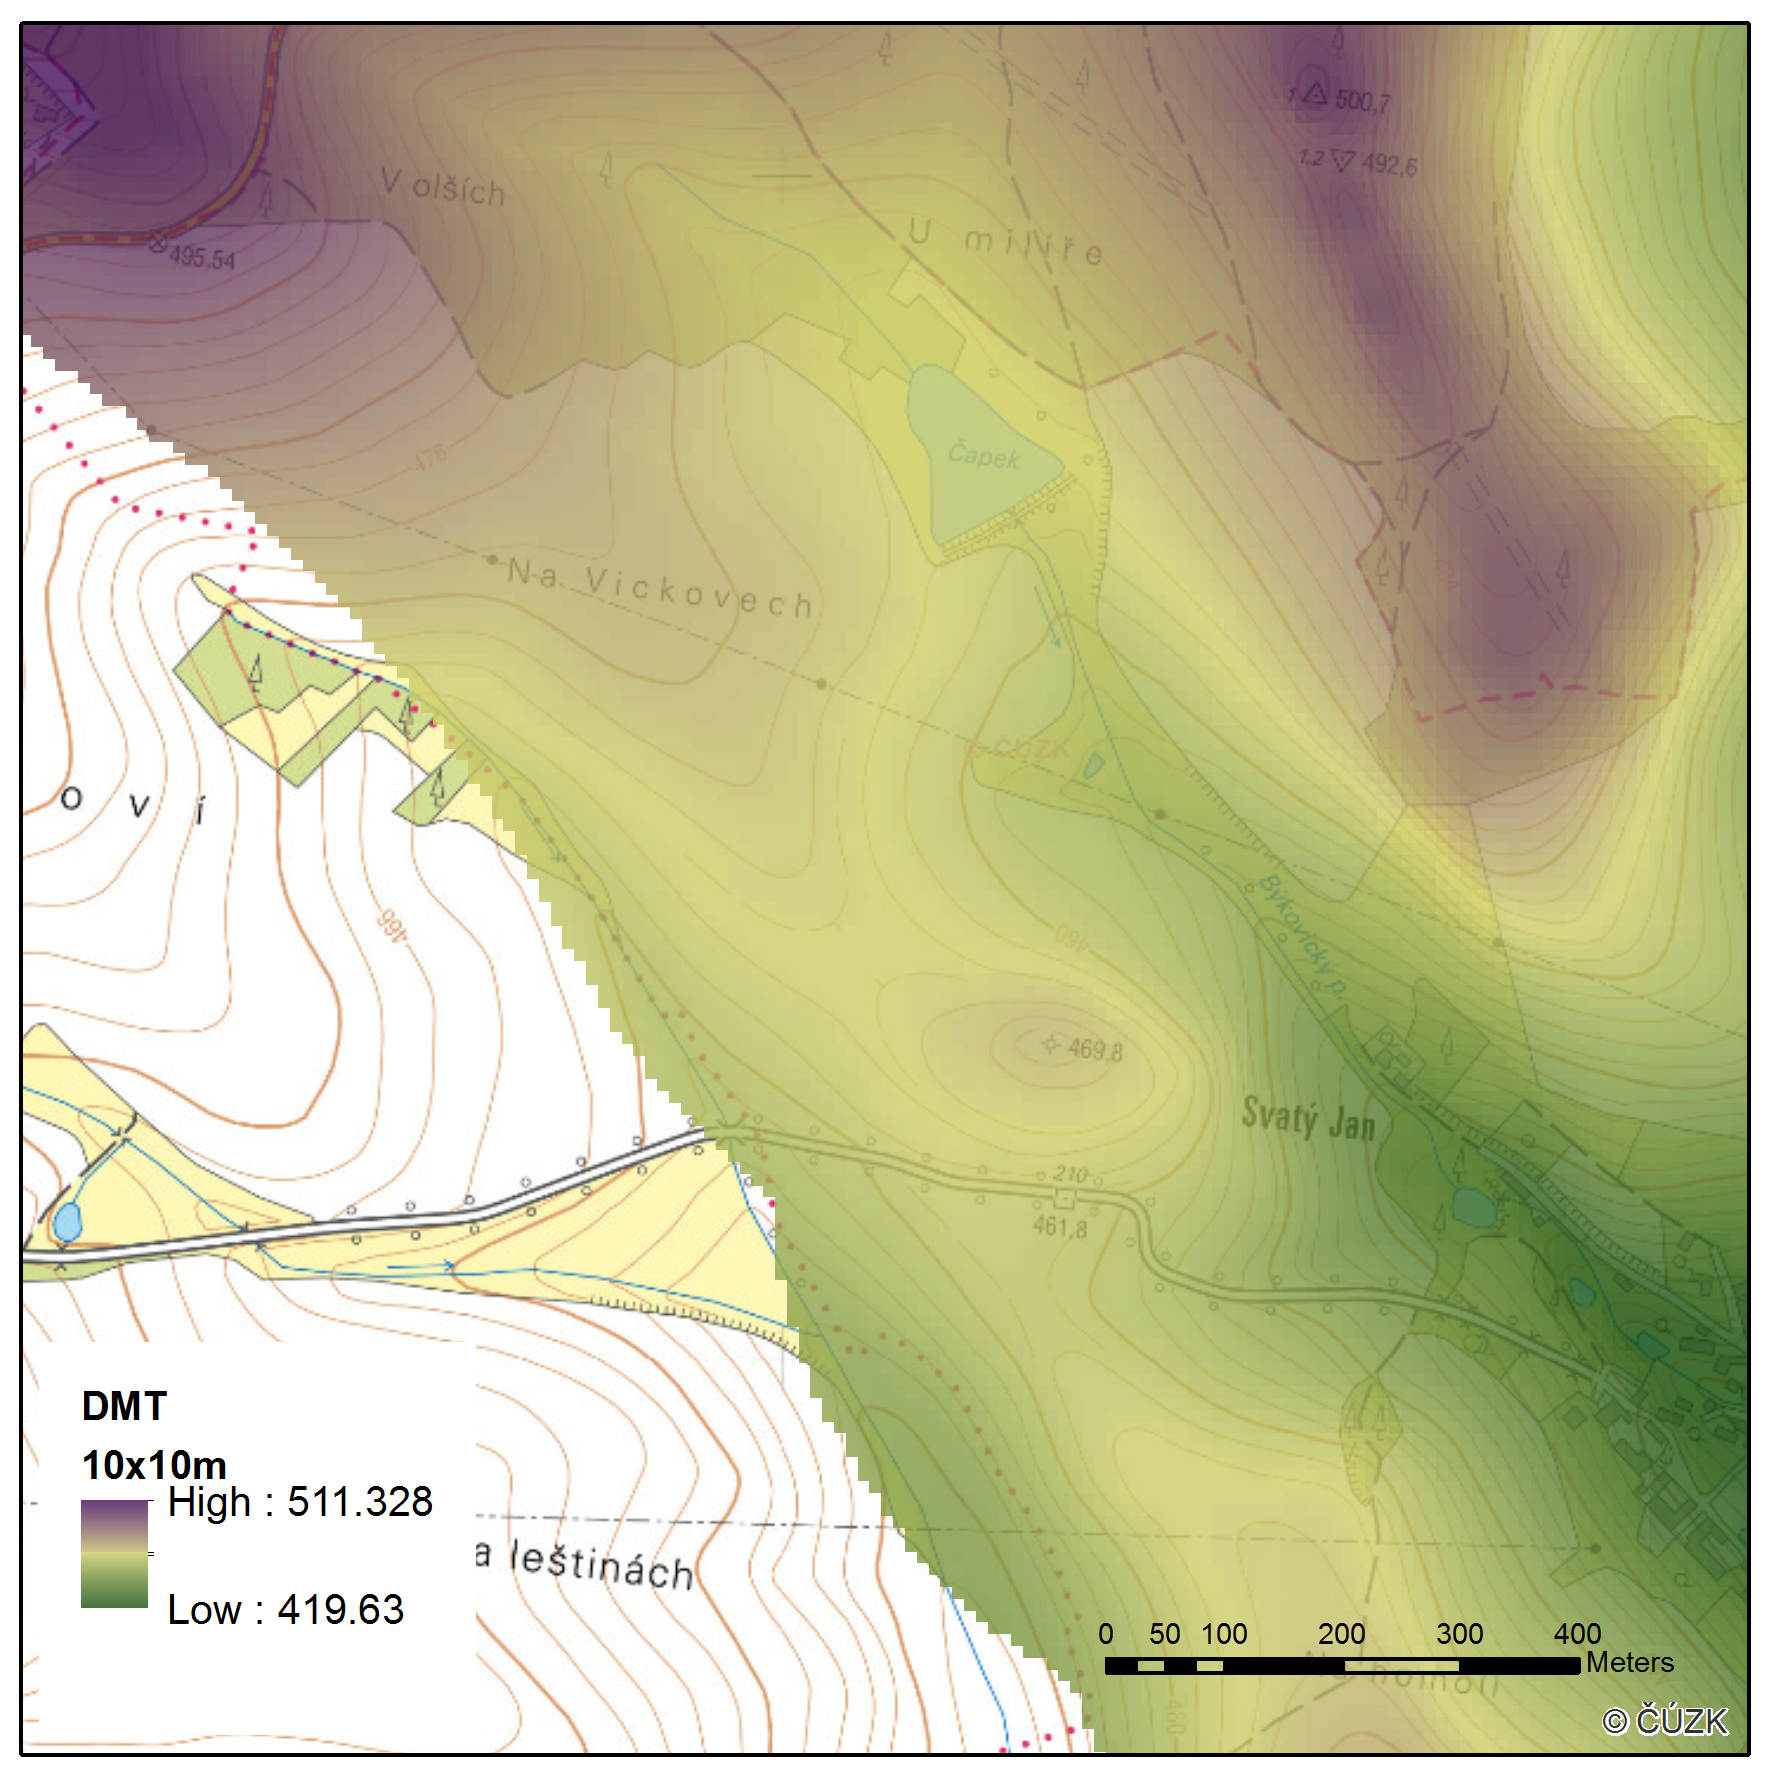
\includegraphics[width=0.5\textwidth]{./img/DMT_byk.png}
%   \caption{Výřez digitálního modelu terénu povodí Býkovice}
%   \label{fig:bykovicedmt}
% \end{figure}

 
 
 
 
 
 
 
 
 
 
 
 
 
 
 
 
 
 
 
\subsection{Půdní data} \label{sec:vstuppuda}

Datové zdroje vlastností půd jsou v rámci České Republiky roztříštěné. Model \smod pracuje s jednou vstupní vrstvou půd. Příprava této vrstvy z dostupných dat je otázkou preprocessingu a propojení relevantních zdrojů. V zásadě jsou tři základní dostupné datové zdroje půdních vlastností. Odděleně připravená \pozn{to: jinou metodou pripravene si nejsem jist} data na zemědělské a lesní půdě nebo bezešvá vrstva půd KPP odpovídající měřítku 1:200000.

V České Republice se na zemědělské půdě standardně využívá klasifikace podle Nováka. Půda je rozdělena podle obsahu jílových částic na půdy \cite{kavka} \pozn{ v bib/bib.bib zadna polozka s oznacenim kavka neni...}:
\begin{itemize} \itemsep -3pt
  \item písčité
  \item hlinitopísčité
  \item písčitohlinité
  \item hlinité
  \item jílovitohlinité
  \item jílovité
  \item jíl
\end{itemize}

Na lesních půdách je v České Republice standardně využíván popis kategorií podle klasifikace USDA\footnote{United States Department of Agriculture}.
Obrázek~\ref{fig:puda} ukazuje výřez připravené vrstvy. Pro určení charakteristik je nutné, aby atributová tabulka dané vrstvy obsahoval identifikátor půdního typu. Identifikátor odkazuje na půdní charakteristiky, které jsou ale uložené ve zvláštní tabulce (viz níže). Mezi půdní charakteristiky a parametry používané modelem patří: \acs{HyVod} - \acl{HyVod}; \acs{Sorb} - \acl{Sorb}; \acs{n} - \acl{n}, \acs{b} - \acl{b}, \acs{X} - \acl{X} a  \acs{Y} - \acl{Y}. Hodnoty těchto parametrů lze převzít z tabulky~\ref{tab:kriticke} v příloze~\ref{sec:priloha}. Fyzikální význam těchto parametrů a jejich implementace v modelu jsou popsány v části~\ref{cast:1} toho manuálu. 





 
 
 
 
 
 
 
 
 
 
 
\subsection{Data využití území} \label{sec:vstupvegetace}
\pozn{pk - doplnit zdroje takovych dat}
Obdobně jako u půdních dat je vstupem vektorový shapefile popisující využití území. Mezi základní typy, pro které byl model testován, patří:
\begin{itemize} \itemsep -3pt
  \item atropogení a zpevněné plochy  
  \item holá půda bez vegetace
  \item les
  \item sad
  \item travní porosty
  \item zemědělské plodiny širokořádkové\footnote{Širokořádkové plodiny jsou například brambory, kukuřice, řepa, sója a slunečnice.}
  \item zemědělské plodiny úzkořádkové\footnote{Úzkořádkové plodiny jsou obiloviny nebo řepka.}
\end{itemize}


Shapefile popisující využití území je ukázán na obrázku~\ref{fig:LU}. Obdobně jako u půd v předchozí sekci je třeba atributovou tabulku tohoto shapefilu doplnit o identifikátor daného využití území. Tento identifikátor odkazuje na charakteristiky daného povrchu definované ve zvláštní tabulce (popsáno v sekci~\ref{sec:upravatabulkyparametru}). Parametry související s využitím území, které vstupující do modelu jsou \acs{PotI} - \acl{PotI} a \acs{Lai} - \acl{Lai}. Jejich konkrétní použití je popsáno v části~\ref{cast:1} toho manuálu. 
% 
% \begin{figure}
%   \centering
%   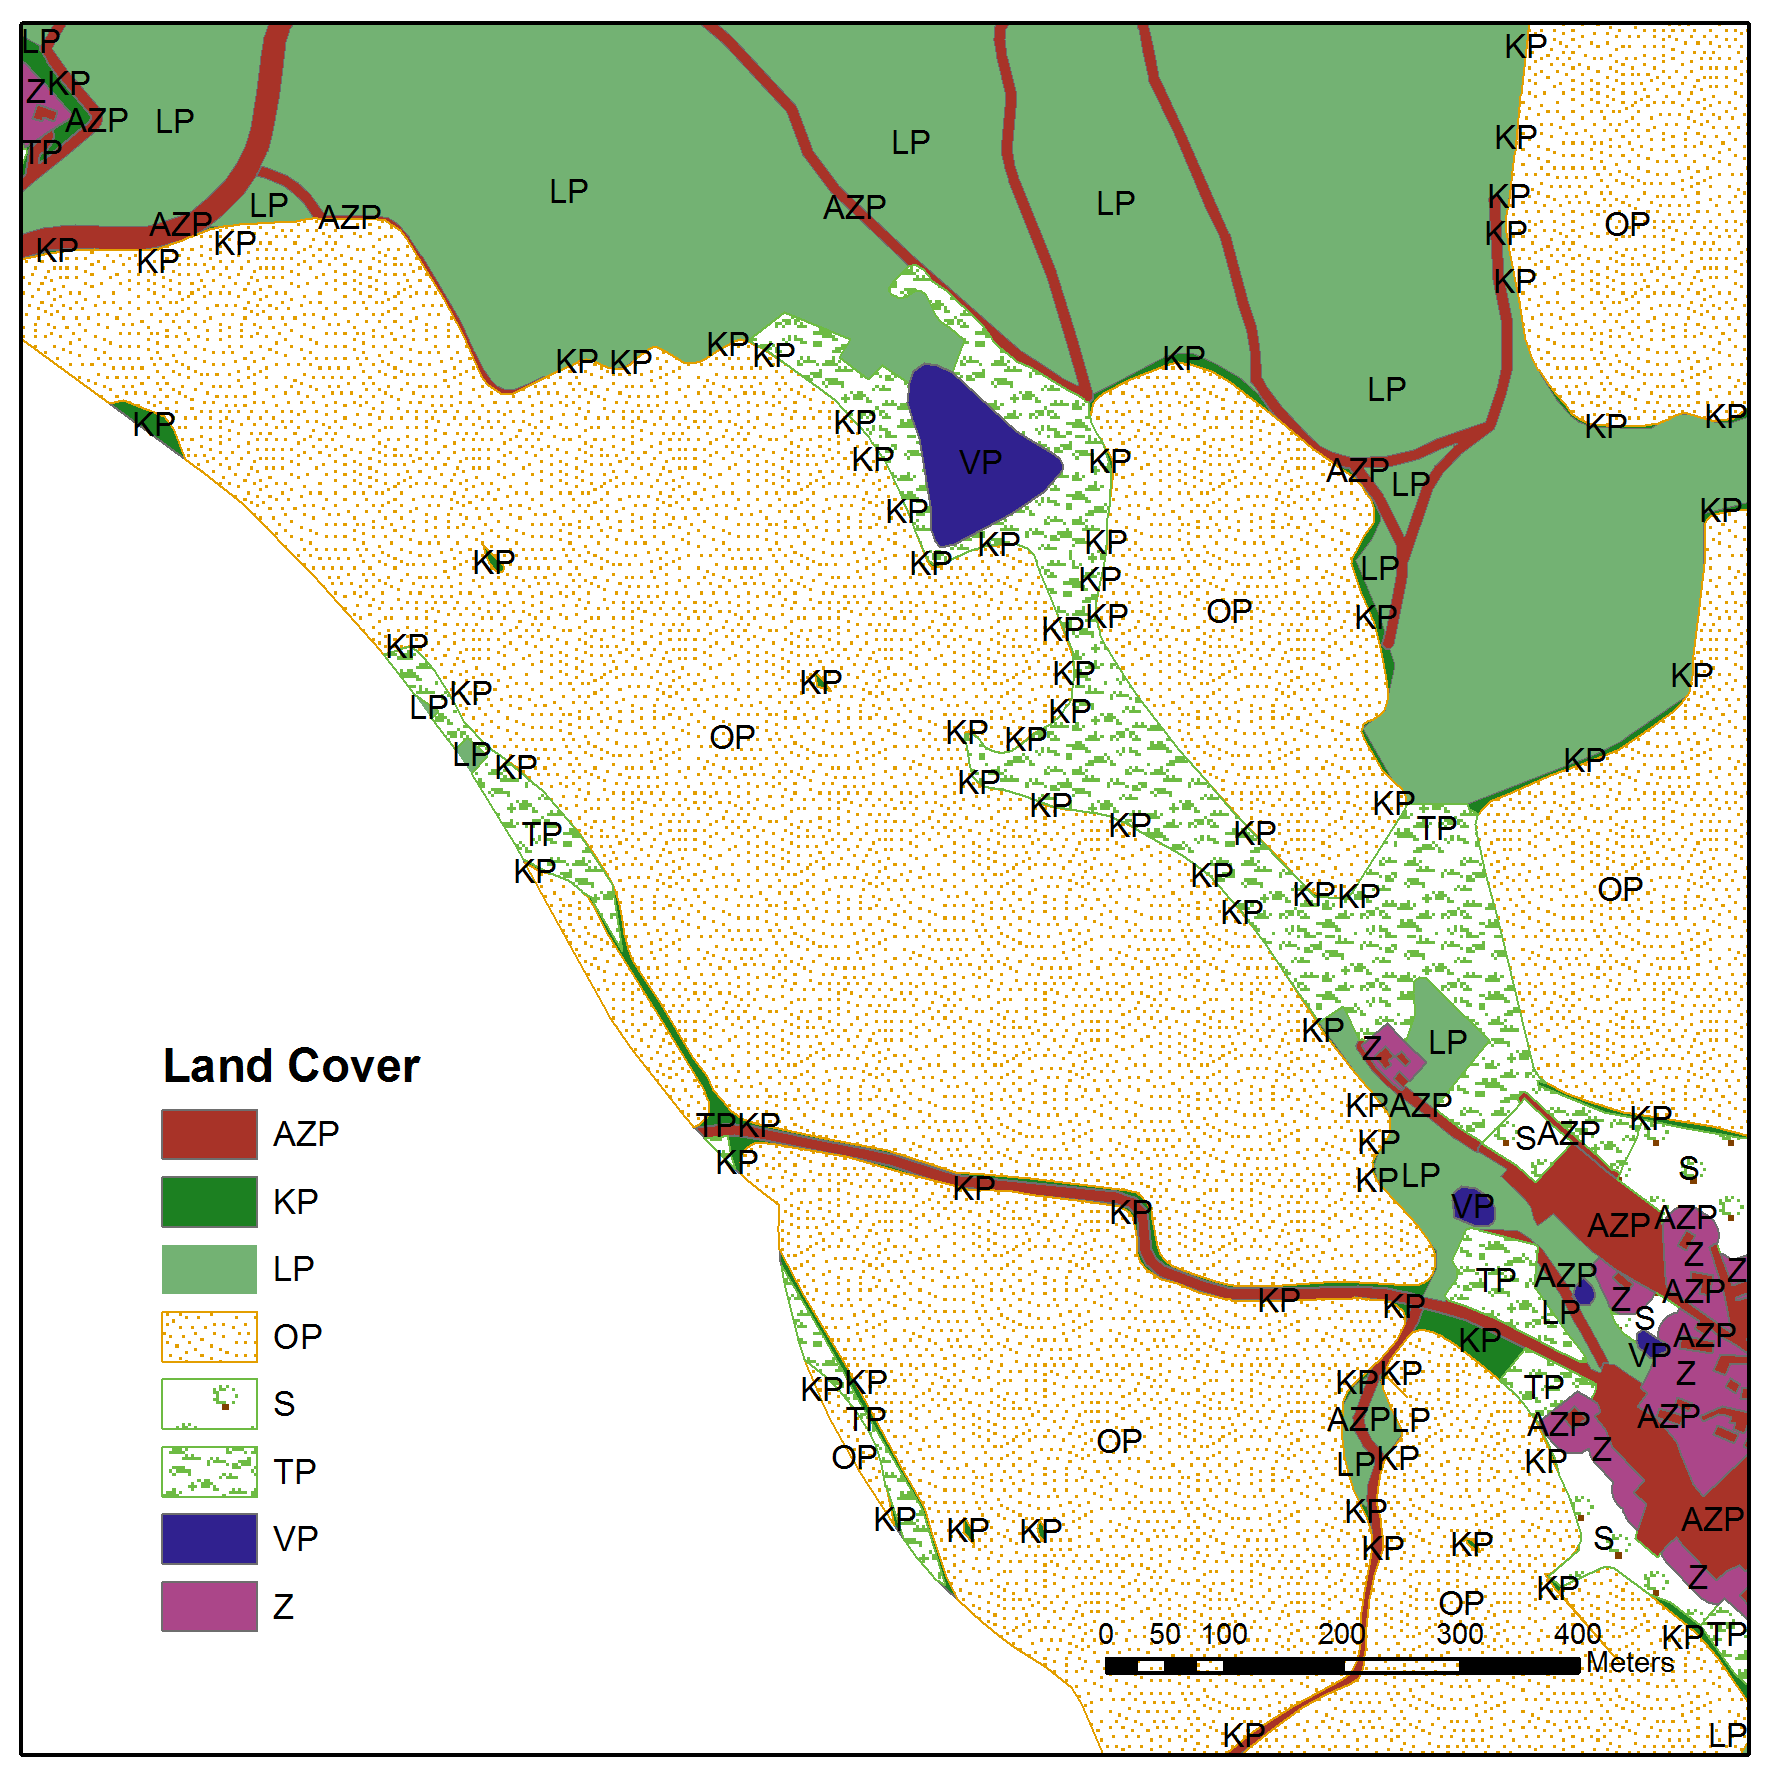
\includegraphics[width=0.5\textwidth]{./img/LandCover.png}
%   \caption{Ukázka vektorové vrstvy využití území -  Land Cover}
%   \label{fig:bykovicevegetace}
% \end{figure}
% 
% 
% 















\subsection{Tabulka parametrů půdy a využití území}  \label{sec:upravatabulkyparametru}

Další povinný vstup je tabulka, která obsahuje hodnoty jednotlivých parametrů popsaných v předešlých kapitolách a části~\ref{cast:1} toho manuálu. Na tuto tabulku se odkazují identifikátory půdního typu a typu využití území definované pro jednotlivé polygony ve vektorových vstupech. Tato tabulka může být do modelu vlože jako textový soubor. Na obrázku~\ref{fig:soilvegtablo} je ukázán příklad takové tabulky. V prvních dvou sloupcích jsou identifikátory ($id$) typu půd ($Soil$) a typu využití území ($Land$ $Co.$). Spojením těchto dvou $id$ jsou označeny parametry pro danou kombinaci typu půdy a využití území (třetí sloupec v tabulce na obrázku~\ref{fig:soilvegtablo} s označením $soilveg$). Toto $id$ je pak spojeno s vektorovou vrstvou na obrázku~\ref{fig:prunik}, kde jsou spojeny $id$ z průniku vektorových vrstev půdy~\ref{fig:puda} a využití území~\ref{fig:LU}. Tyto prostorově distribuované parametry jsou následně pro potřeby výpočtu uloženy do rastrů. Význam jednotlivých veličin je popsán v tabulce~\ref{tab:soilveg}. Při přípravě dat je nutné dodržet označení parametrů v této tabulce!

% Na prvním řádku je ukázka odpovídající id půdního typu z obrázku~\ref{fig:bykovicepuda} HP a id typu využití území z obrázku~\ref{fig:bykovicevegetace} TP, které jsou v tabulce na obrázku~\ref{fig:tabsoilveg} spojeny na HPTP. Tímto způsobem je program schopen propojit prostorové uspořádání pud a typu vegetace s příslušnými charakteristikami. Spojení identifikátorů z atributových tabulkách polygonových vrstev prování program automaticky. Uživatel musí pouze zaručit aby se identifikátory v nastavené v atributových tabulkách polygonových vrstev schodovali s identifikátory v tabulce půdních charakteristik a charakteristik vegetace. Princip přípravy a propojení rozložení typů a vegetačního pokryvu s odpovídajícími parametry je naznačen na obrátku~\ref{}
% 
% Hlavničky druhého až posledního sloupce jsou povinné. Jejich význam je popsán v tabulce~\ref{tab:soilve g}. Názvy v druhém až posledním sloupečku musí být zadány malými písmeny.
% \begin{figure}
%   \centering
%   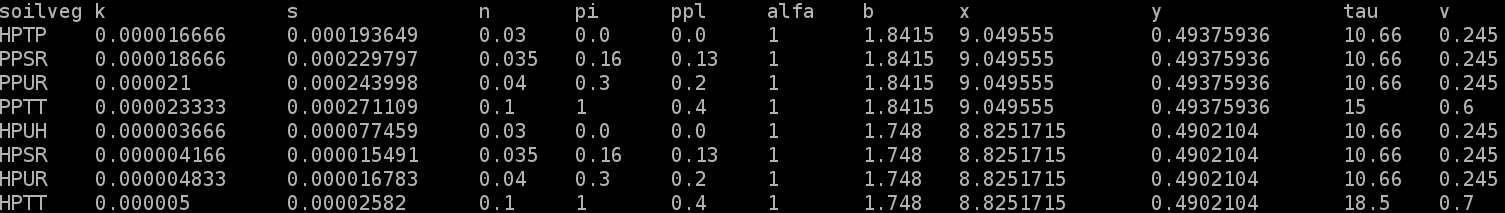
\includegraphics[width=1.0\textwidth]{./img/tabsoilveg.png}
%   \caption{Ukázka tabulky s charakteristikami půd a vegetace. Význam veličin v jednotlivých sloupcích je popsán v tabulce~\ref{tab:soilveg}.}
%   \label{fig:tabsoilveg}
% \end{figure}


% \begin{figure}
%   \centering
%   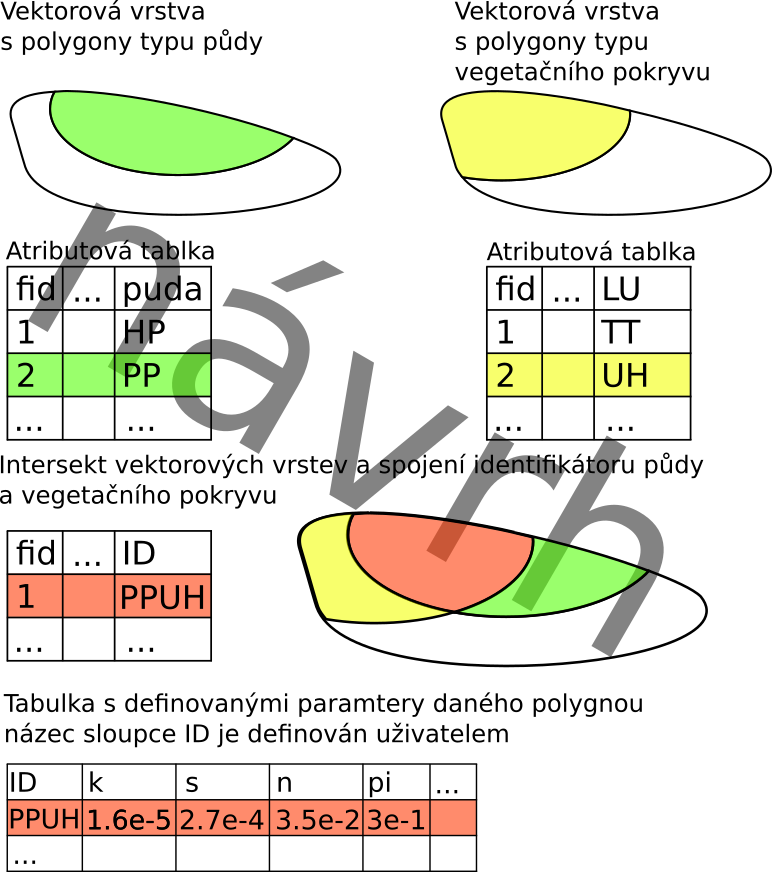
\includegraphics[width=0.75\textwidth]{./img/spojenistabulkou.png}
%   \caption{Princip propojení atributových tabulek vektorových vrstev s tabulkou obsahující jednotlivé parametry}
%   \label{fig:pripravapar_detail}
% \end{figure}



\begin{figure}[t!]
  \centering

  \begin{subfigure}[b]{0.4\linewidth}
    \centering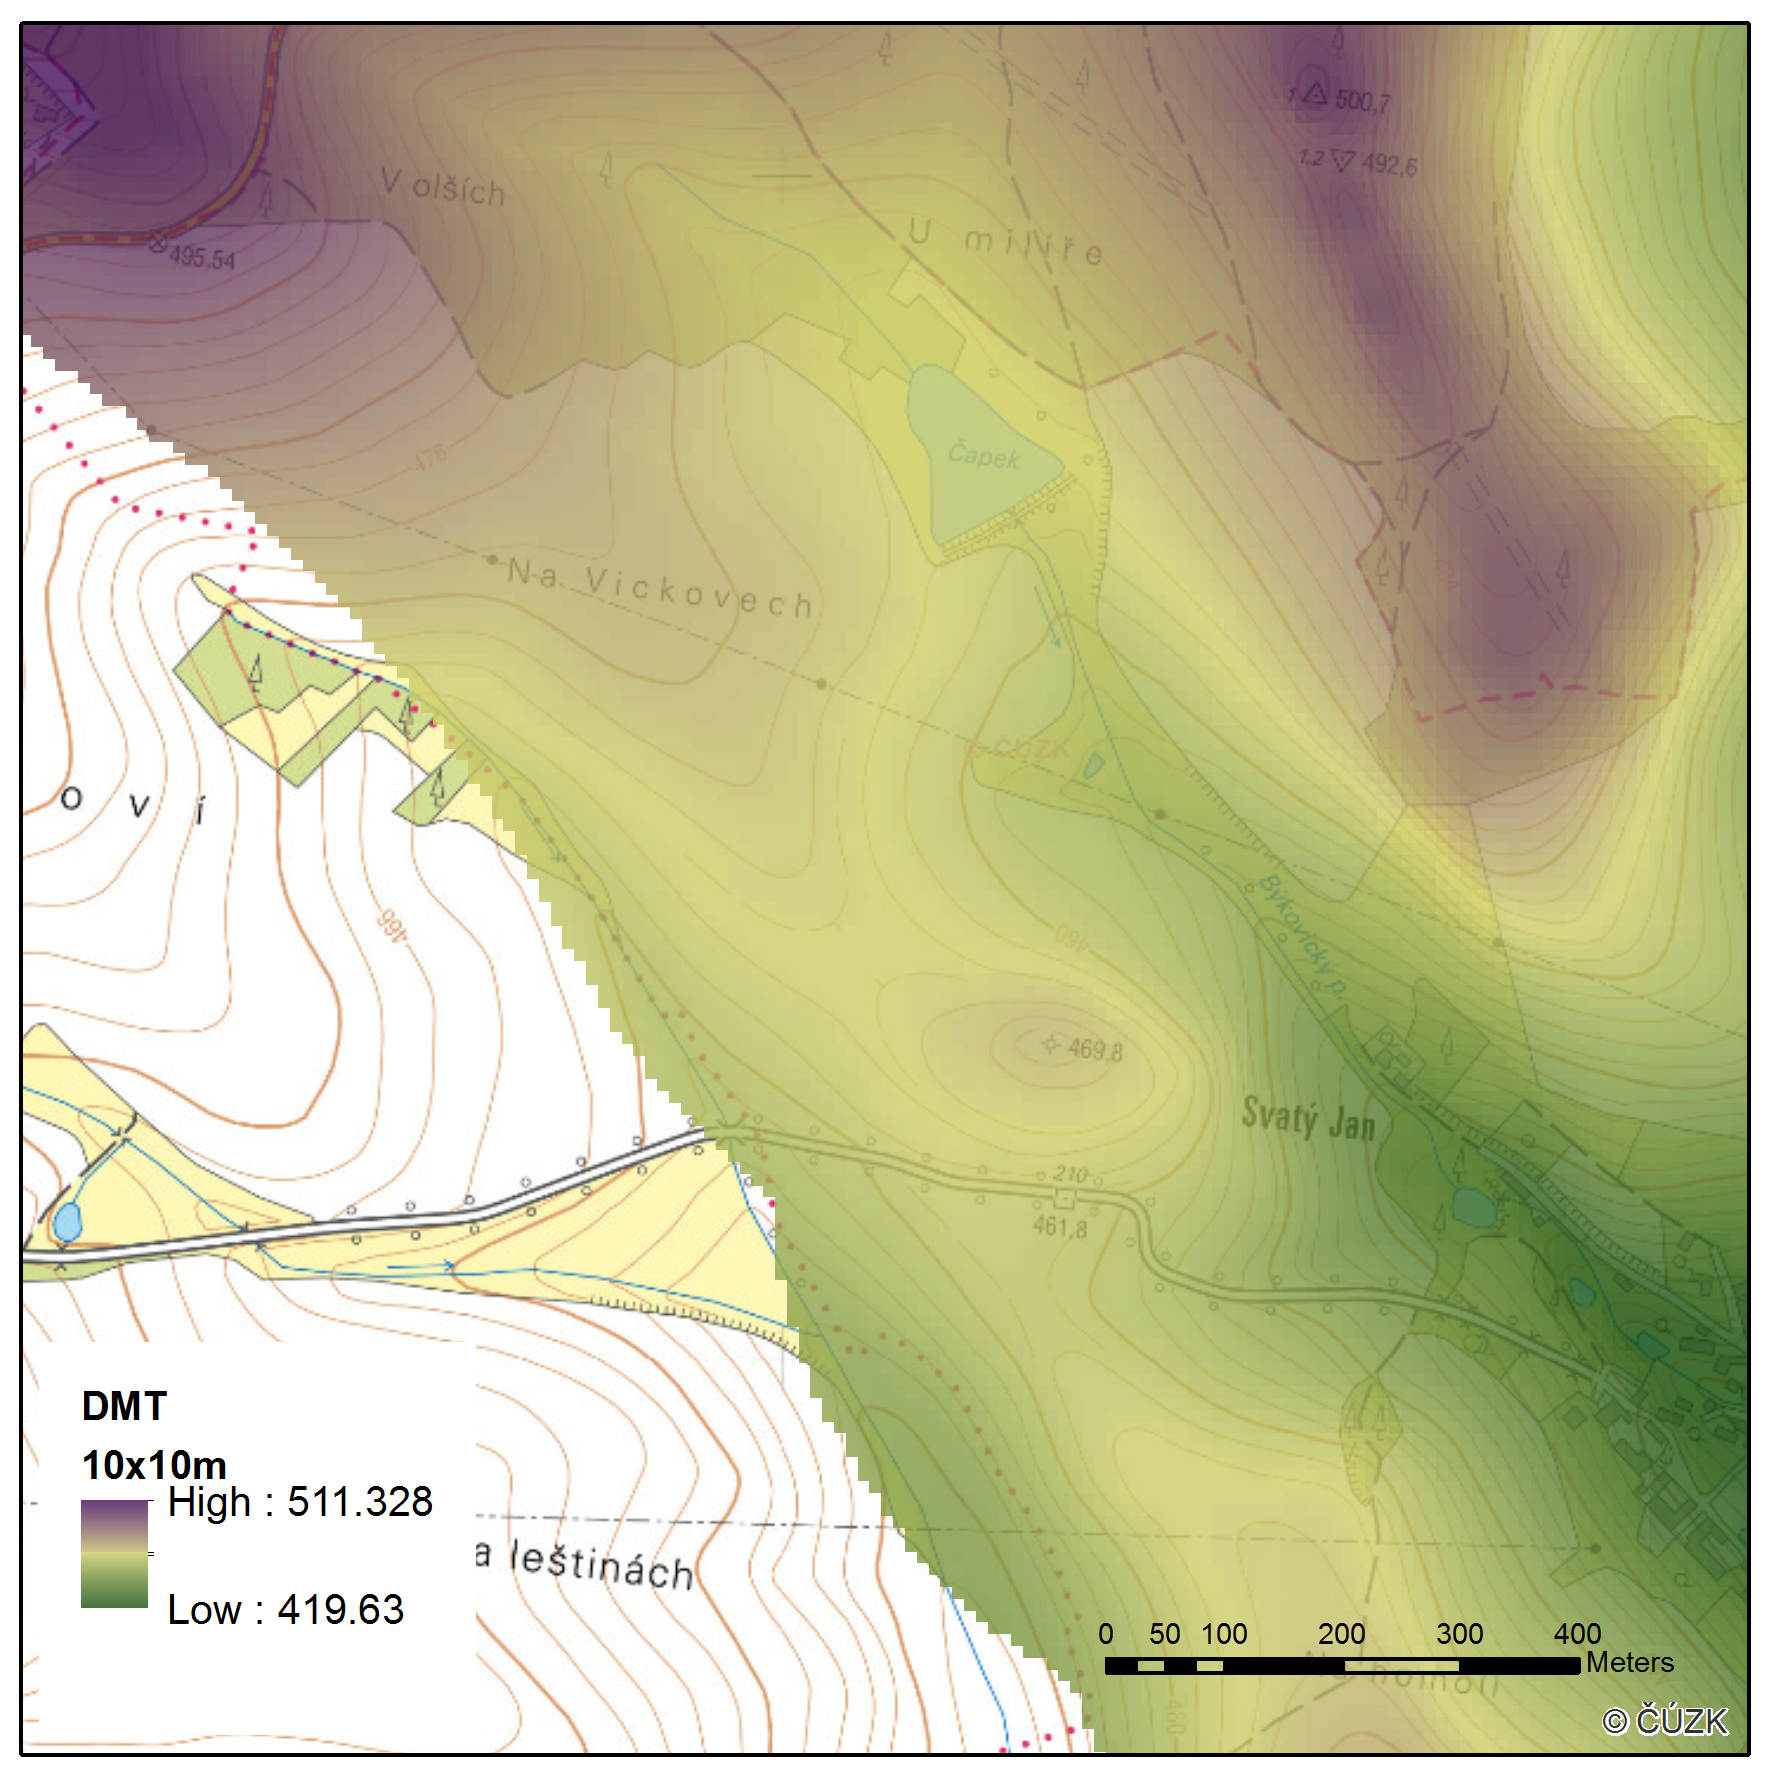
\includegraphics[width=1\linewidth]{./img/DMT_byk.png}
    \caption{\label{fig:dmt}}
  \end{subfigure}%
  \begin{subfigure}[b]{0.4\linewidth}
    \centering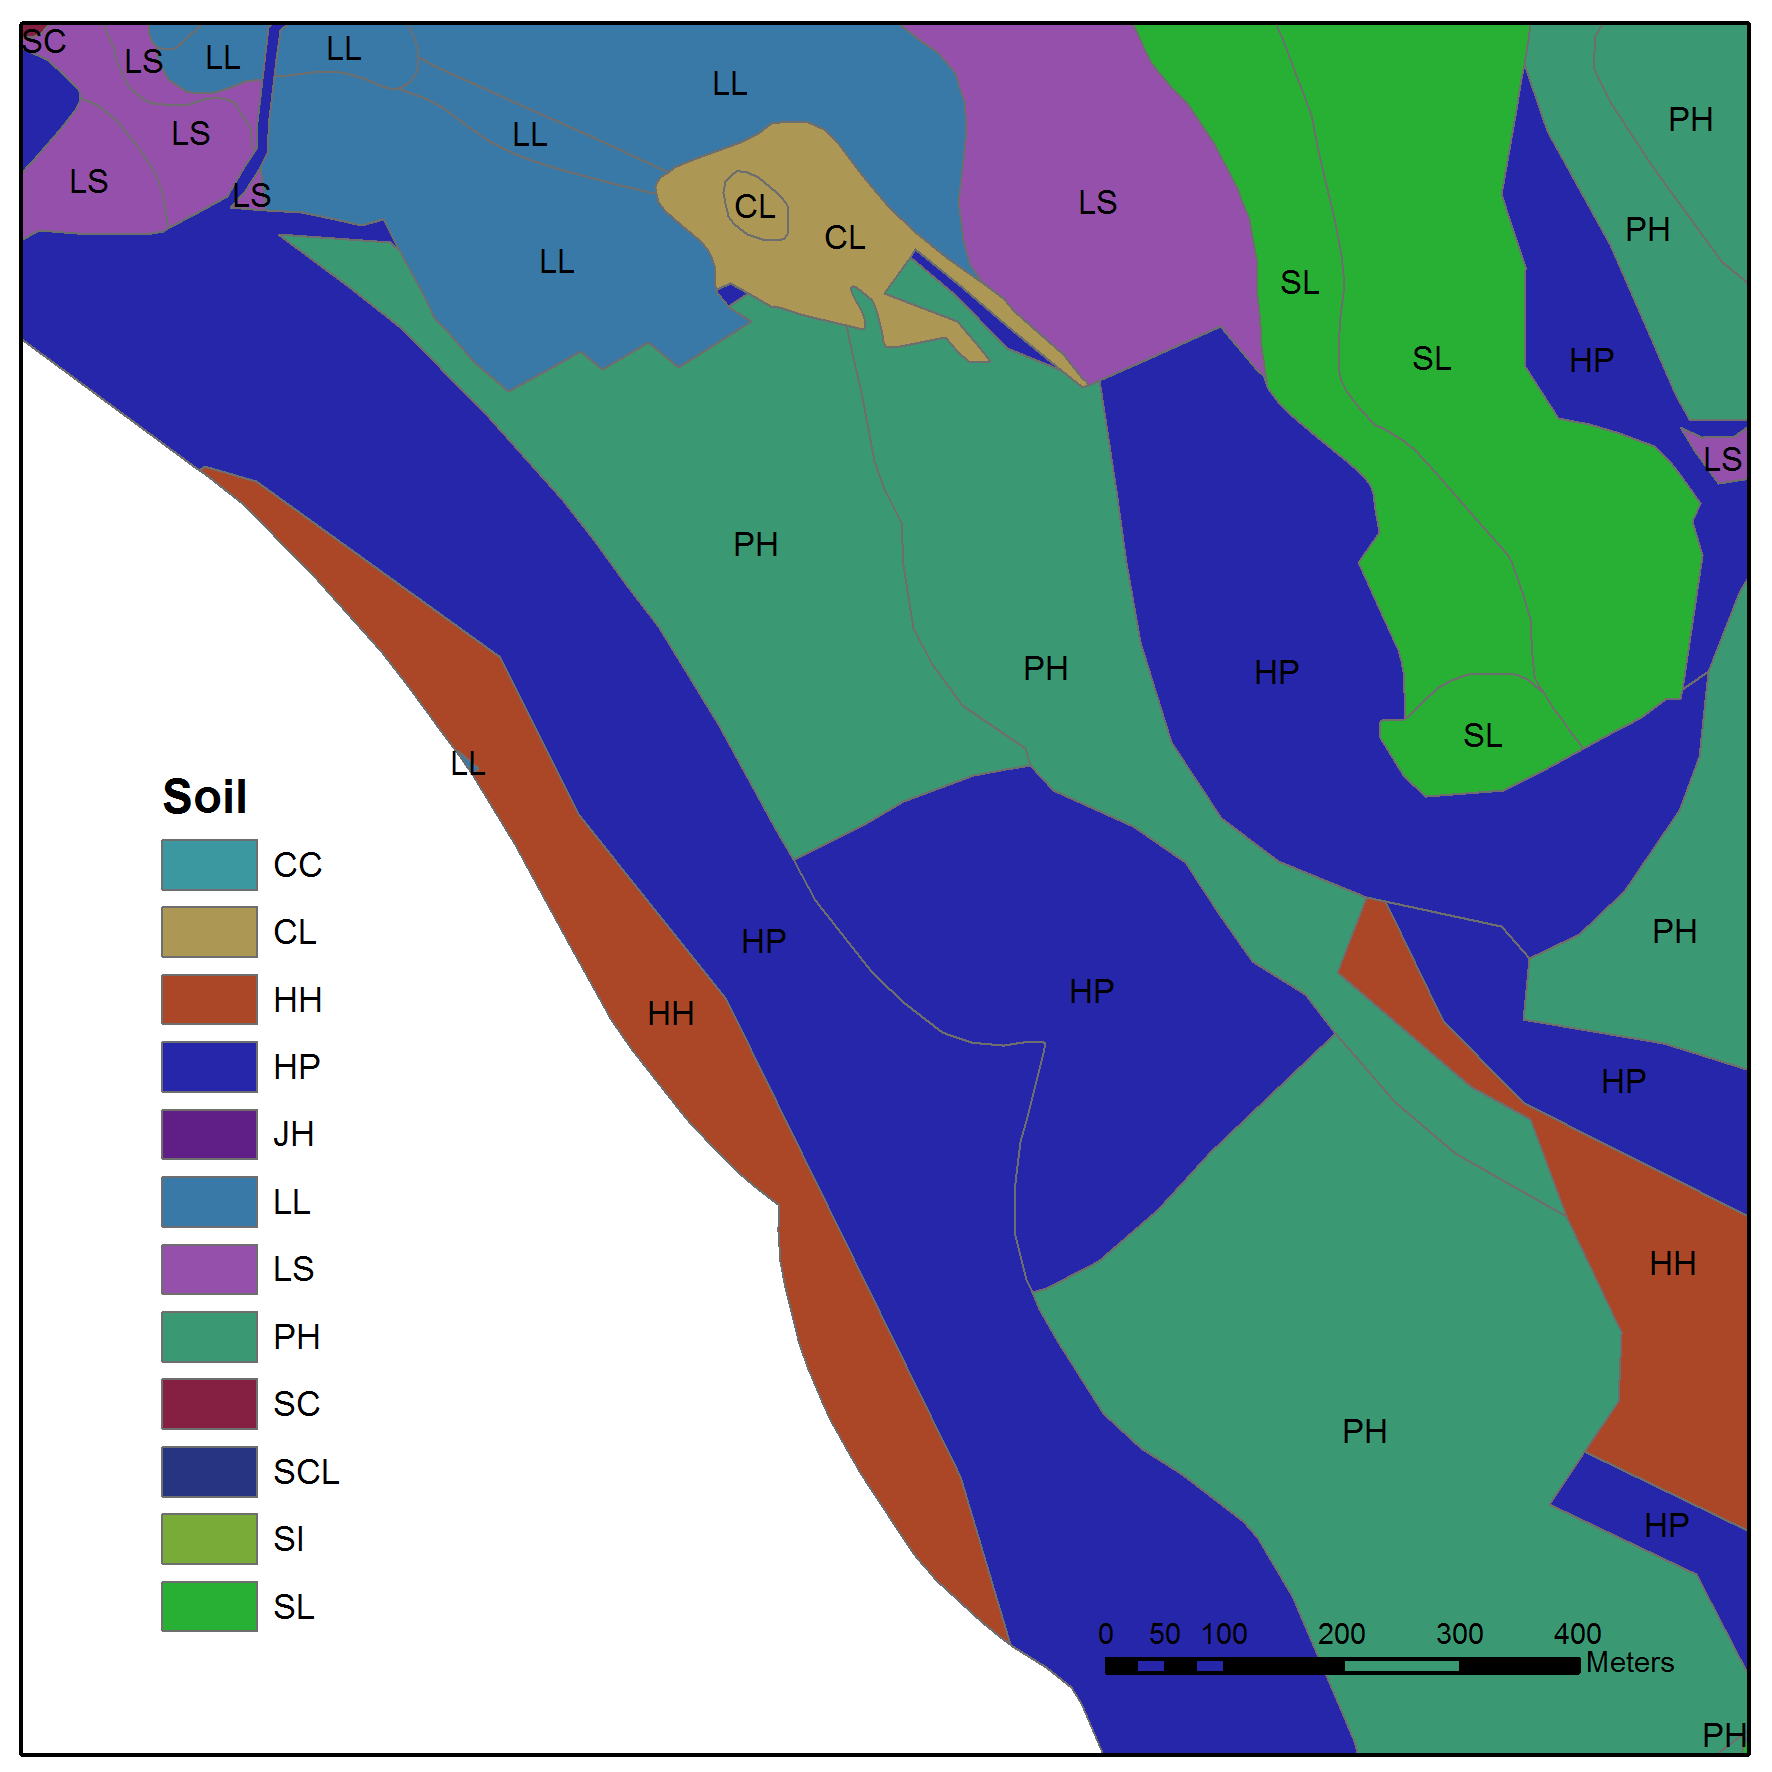
\includegraphics[width=1\linewidth]{./img/pudy.png}
    \caption{\label{fig:puda}}
  \end{subfigure}\\
  \begin{subfigure}[b]{0.4\linewidth}
    \centering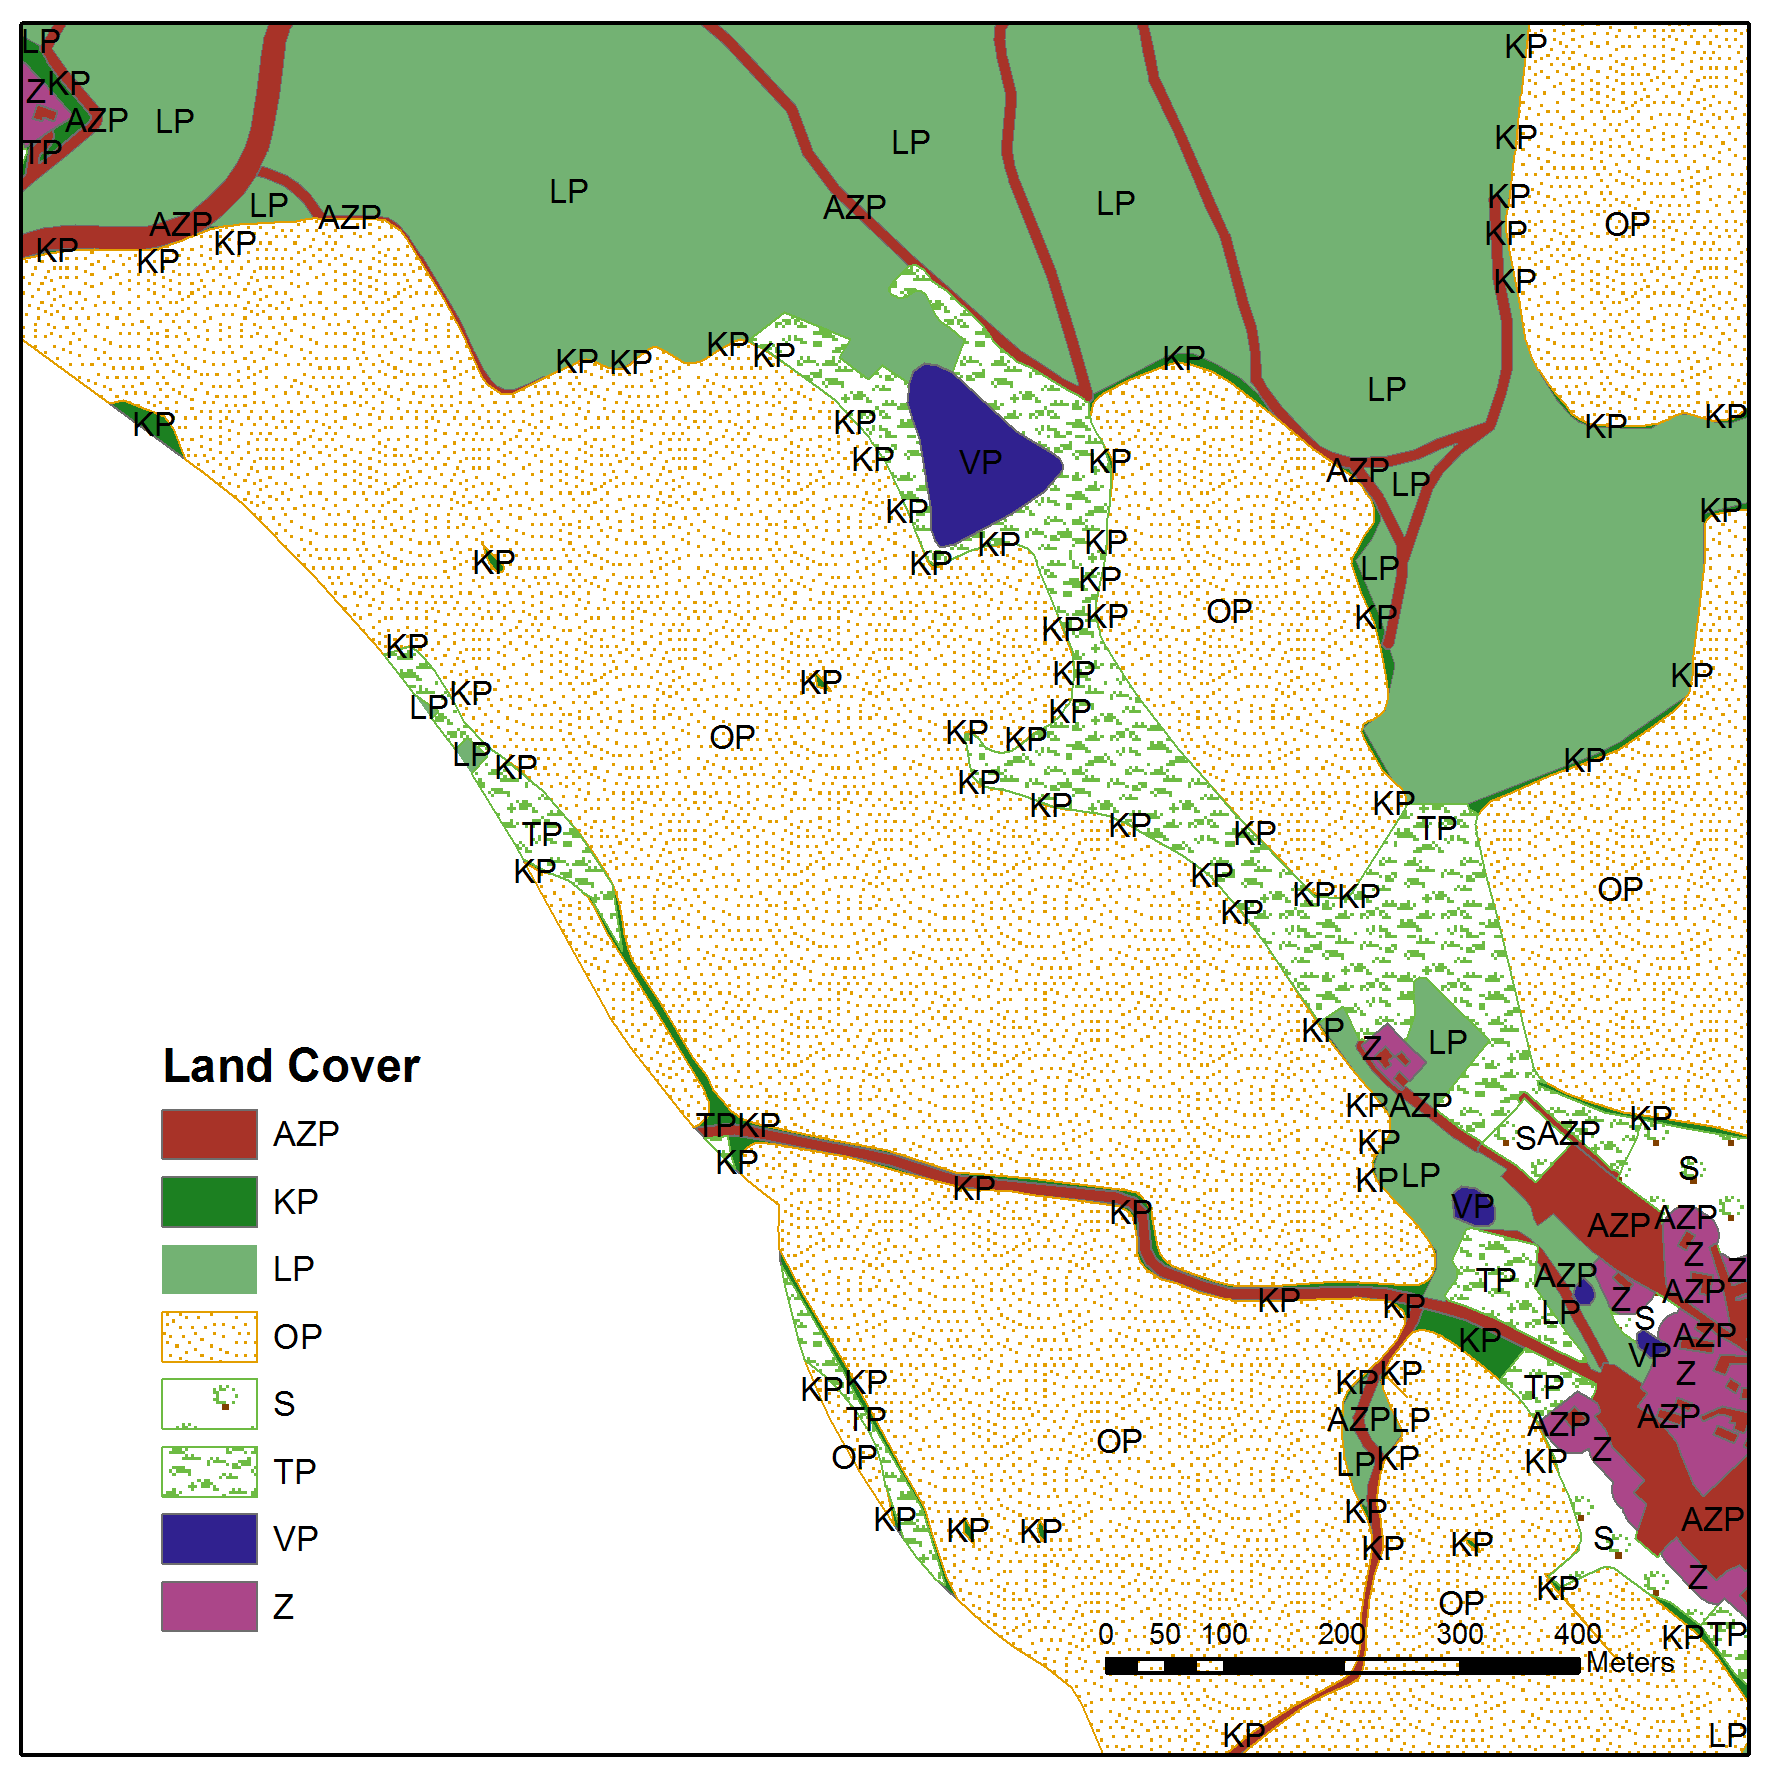
\includegraphics[width=1\linewidth]{./img/LandCover.png}
    \caption{\label{fig:LU}}
  \end{subfigure}%
  \begin{subfigure}[b]{0.4\linewidth}
    \centering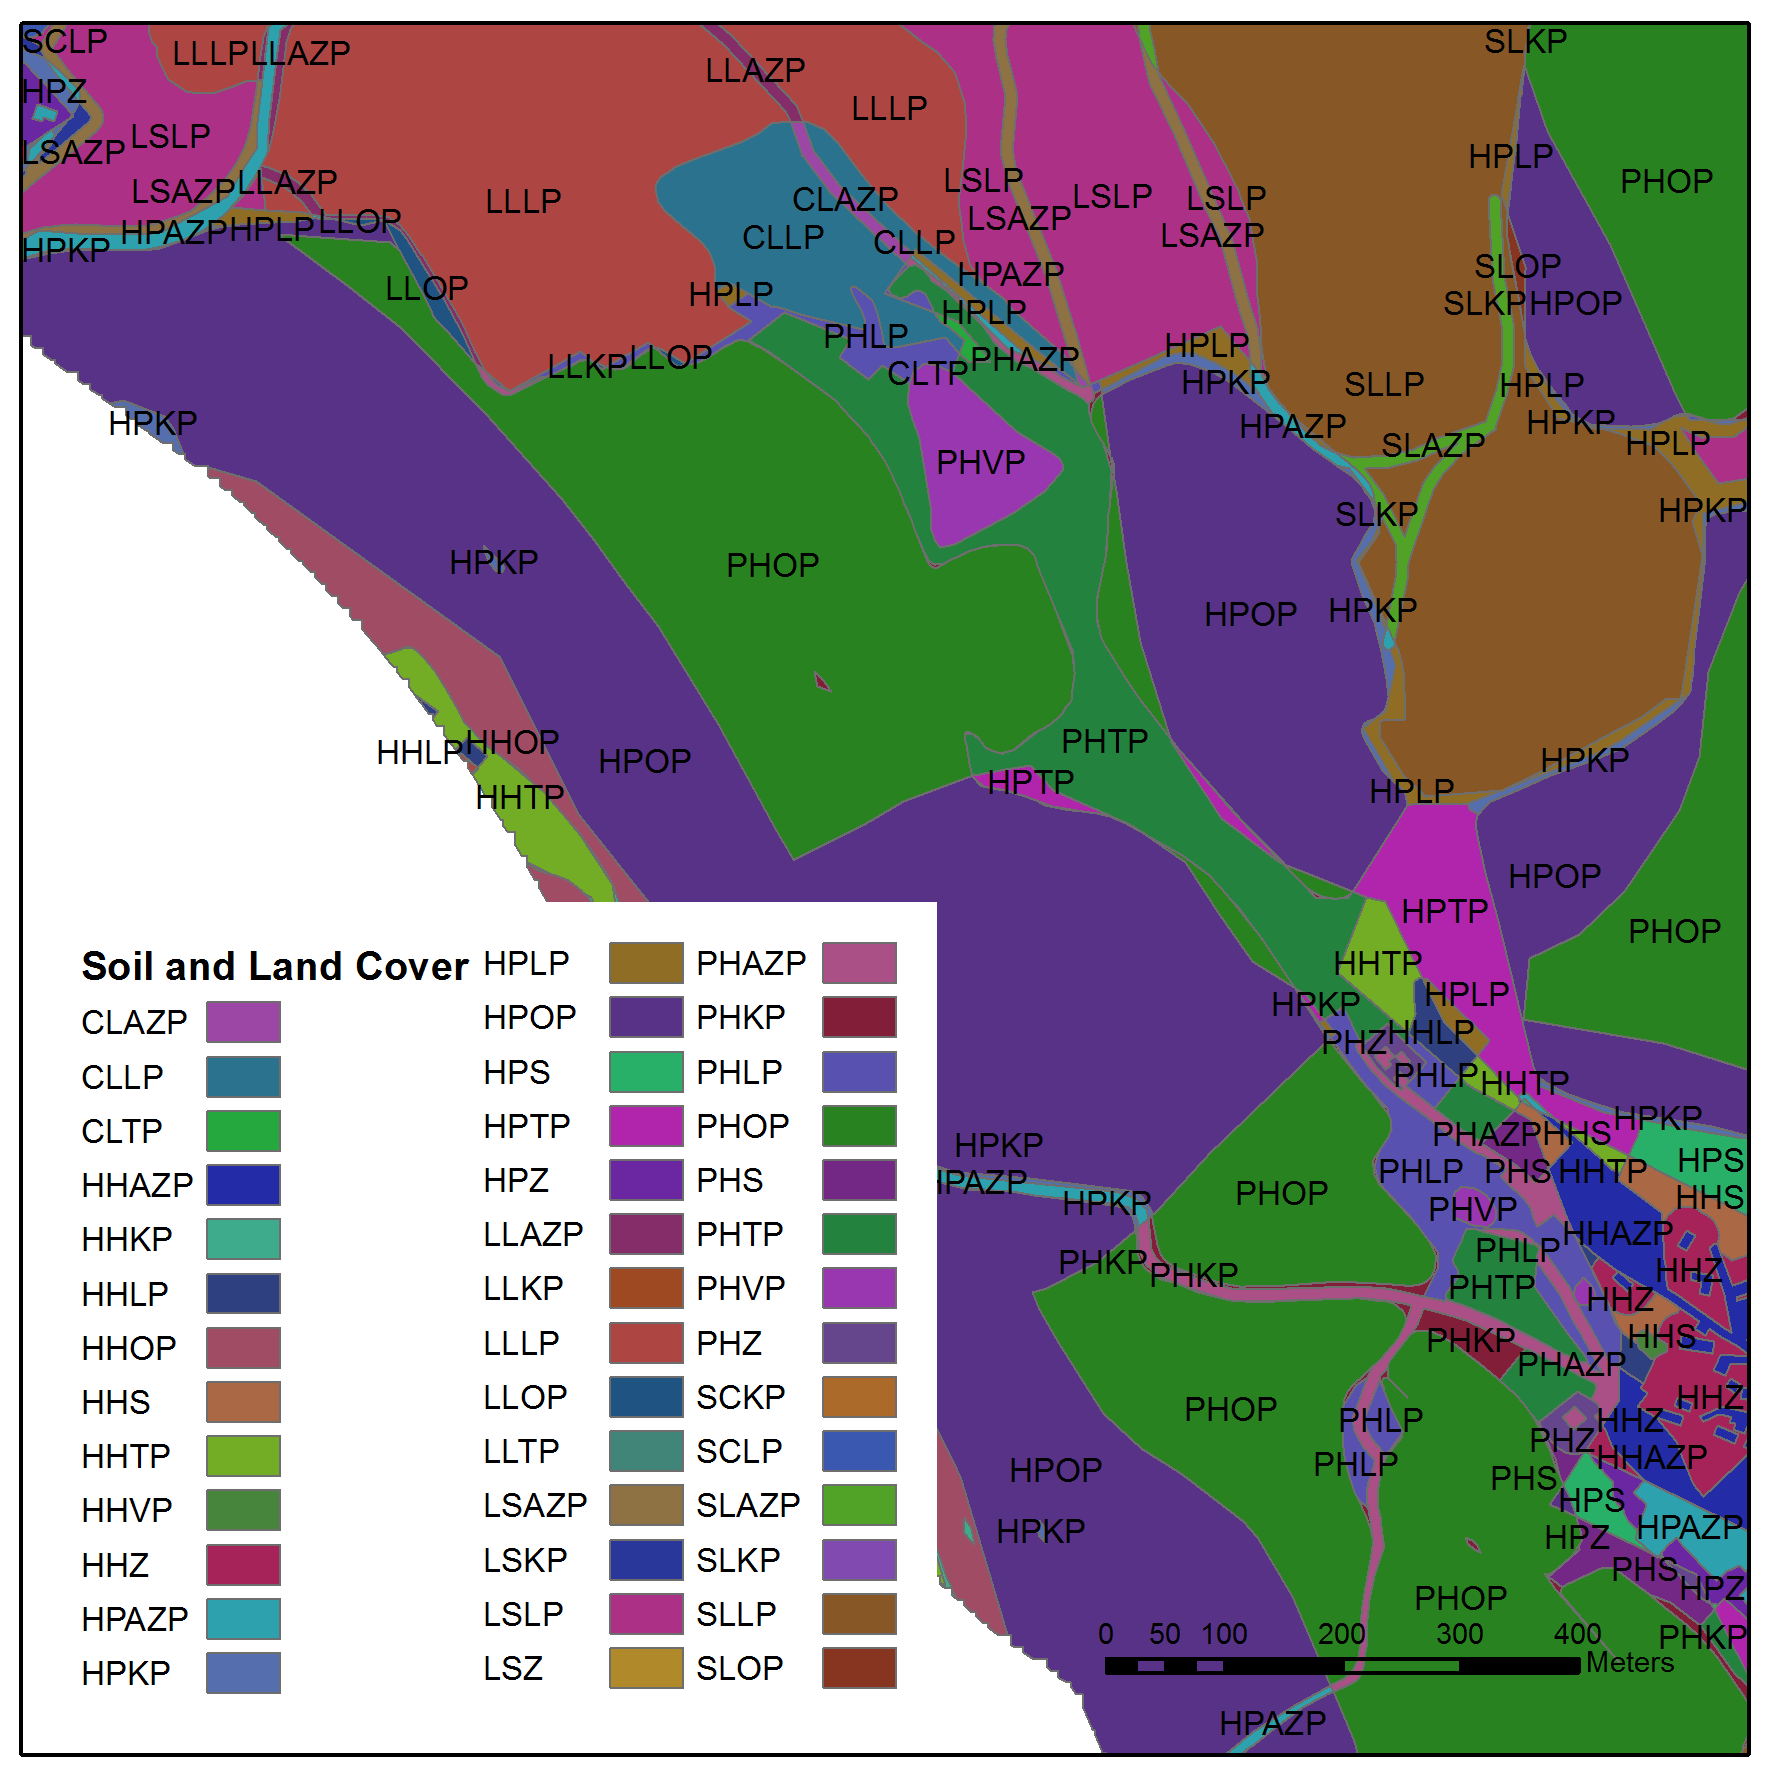
\includegraphics[width=1\linewidth]{./img/SoilAndLC.png}
    \caption{\label{fig:prunik}}
  \end{subfigure}\\
  \begin{subfigure}[b]{0.8\linewidth}
    \centering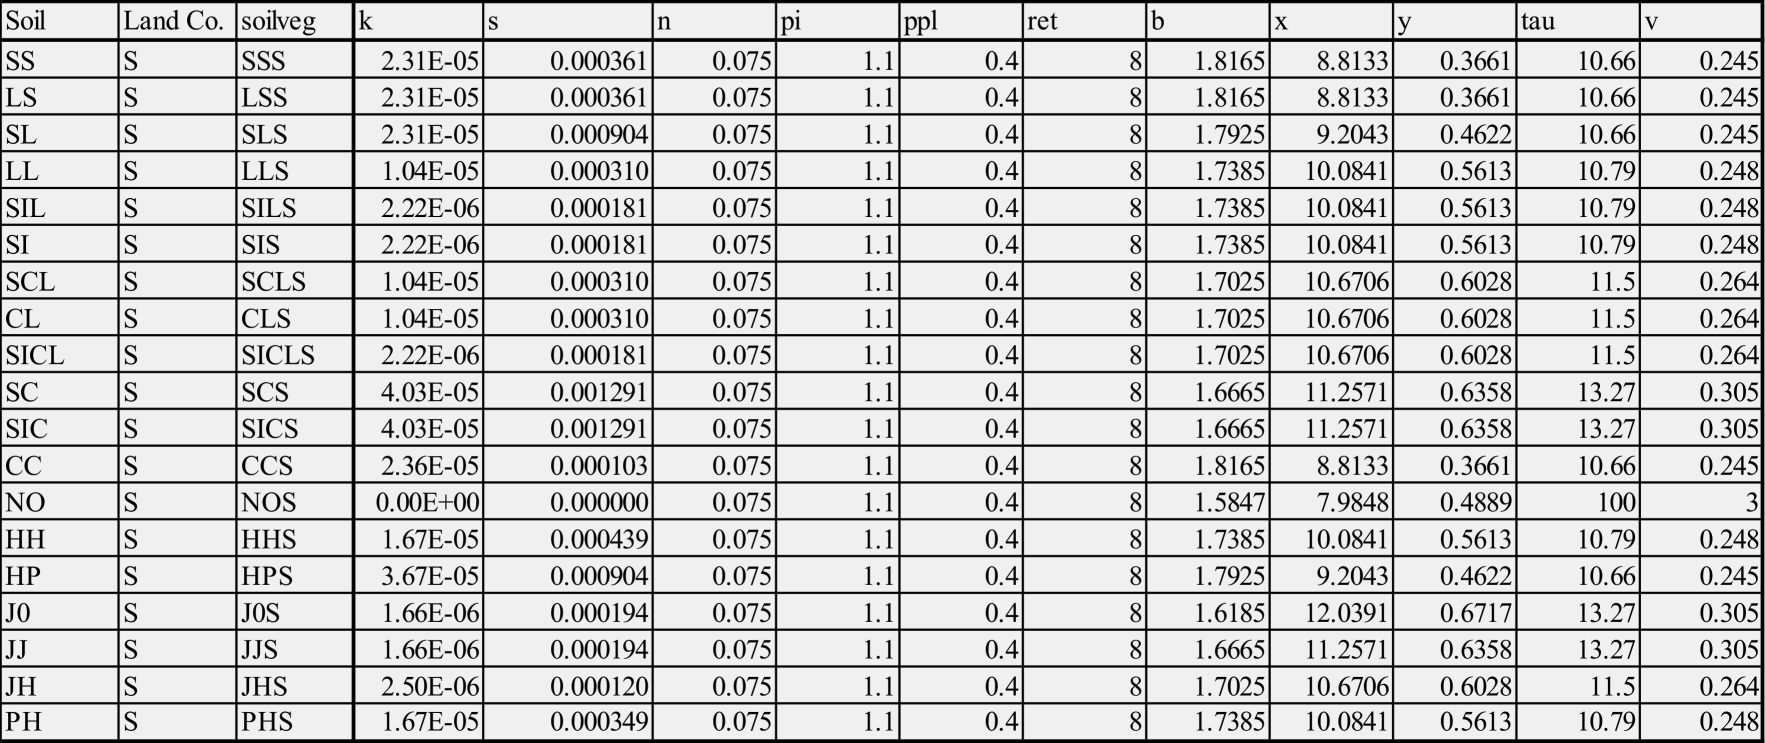
\includegraphics[width=1\linewidth]{./img/soilvegtablo.png}
    \caption{\label{fig:soilvegtablo}}
  \end{subfigure}%
  \caption{Princip propojení vektorových vrstev s tabulkou obsahující parametry typu půd a využití území. Na obrázku a) je digitální model terénu a podkladová mapa. Na obrázku b) je rozložení typu půdy a na obrázku c) rozložení typu využití území. Tyto 2 vrstvy jsou protnuty ($intersect$). Nové polygony převezmou označení z původních vrstev na obrázku b) a c). Tato nová vektorová vrstva je ukázána na obrázku d). Pomocí převzatých označení polygonů jsou k nim přiřazeny parametry typu půd a využití území z tabulky e)}
  \label{fig:soillu}
\end{figure}



\begin{table}%[!htp]
  \centering
  \caption{Přehled parametrů charakterizujících půdní typ a typ vegetačního pokryvu}
  {\small
    \begin{tabular}{p{1.5cm}lp{4cm}}
    \hline
    Hlavička v tabulce & Symbol & Popis \\
    \hline \hline
    k&\acs{HyVod}  & \acl{HyVod} \\
    s&\acs{Sorb}   & \acl{Sorb} \\
    n&\acs{n}      & \acl{n}\\
    pi&\acs{PotI}   & \acl{PotI}\\
    ppl&\acs{Lai}    & \acl{Lai} \\
    ret&\acs{ret}    & \acl{ret} \\
    b&\acs{b}      & \acl{b} \\
    x&\acs{X}      & \acl{X} \\
    y&\acs{Y}      & \acl{Y} \\
    tau&\acs{taucrit}& \acl{taucrit} \\
    v&\acs{vcrit}  & \acl{vcrit} \\
    \hline
    \end{tabular}%
  }
  \label{tab:soilveg}%
\end{table}%



\pozn{tabulka parametru v priloze, vymazal jsem smerodatne odchylky, mam vratit?}





















\subsection{Srážková data} \label{sec:vstupsrazka}

Dalším vstupem je soubor obsahující srážková data. 
% 
% Na obrázku níže je ukázka textového souboru obsahující proměnlivou srážku, konkrétně je to měření na~rastru Býkovic ze~dne 8.2.2010.
%\begin{figure}[hbt]
%  \centering
 % \includegraphics[scale=1]{obrazky/srazkovysoubor.png}
  %\caption{Srážkový soubor}
%  \label{fig:srazkovysoubor}
%\end{figure}
% 
% 
Srážky se zadávají jako textový soubor se dvěma sloupci. V levém sloupci je časový interval v minutách v pravém sloupci je \textbf{kumulativní úhrn} za daný časový interval v \textbf{milimetrech}. Ukázka jednoduché srážky a grafické reprezentace kumulativních dat jsou zobrazeny na obrázku~\ref{fig:srazkovysoubor}. 
\begin{figure}
  \centering
  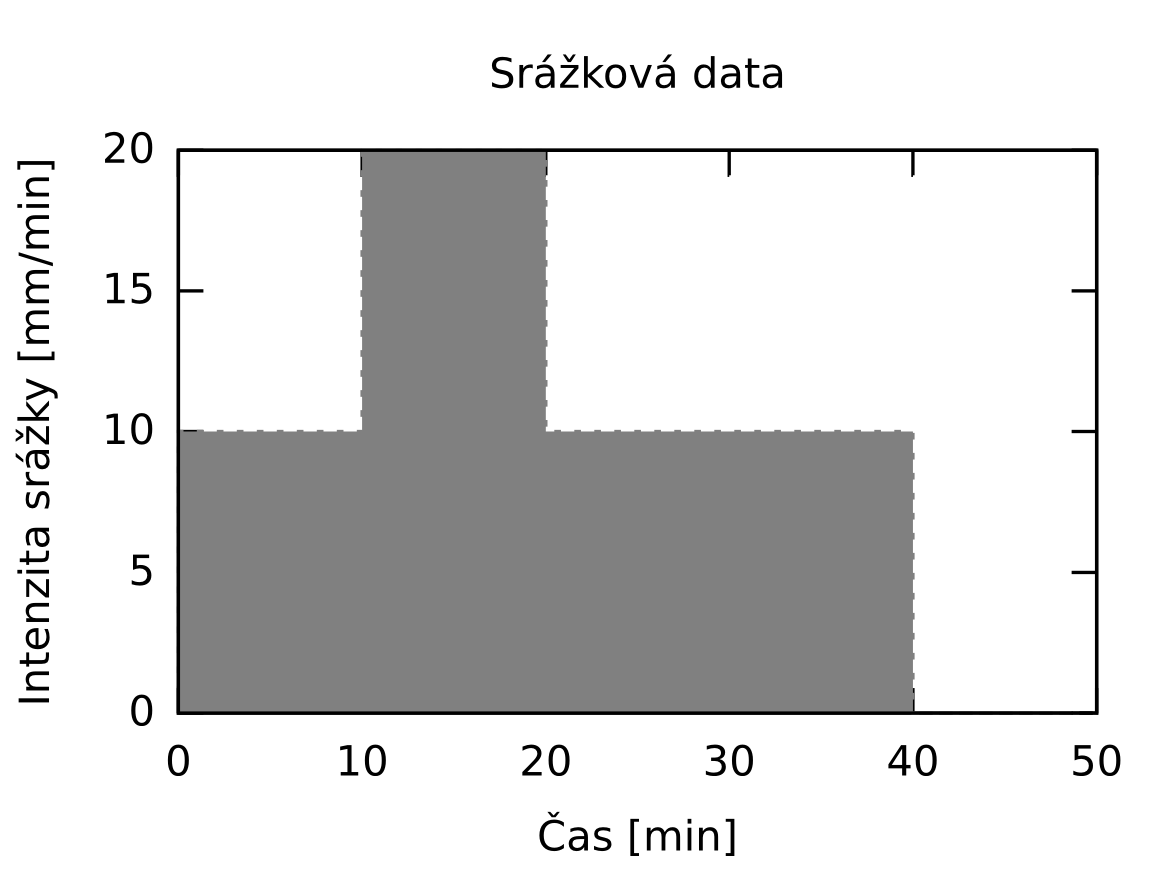
\includegraphics[width=0.45\textwidth]{./img/srazka-graf.png}
  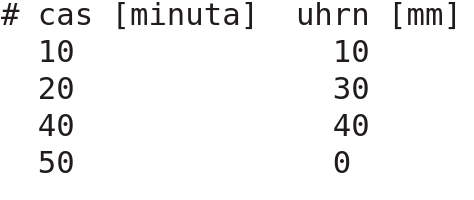
\includegraphics[width=0.5\textwidth]{./img/srazka-soubor.png}
  \caption{Ukázka srážkových dat. Vlevo: grafická reprezentace zadaných dat (srážka zobrazena v intenzitách; Napravo: ukázka dat v požadovaném formátu)}
  \label{fig:srazkovysoubor}
\end{figure}














\subsection{Časový krok modelu a celková doba výpočtu} \label{sec:vstupkrok}

Časový krok modelu označený \acs{dT} je hodnota v sekundách. Jako vstupní parametr se zadává maximální časový krok. Tento časový krok je rovněž počáteční časový krok. Časový krok \acs{dT} je v průběhu výpočtu upravován podle Courant-Friedrich-Lewy (\acs{CFL}) podmínky tak, aby byla zachována numerická stabilita. Délka časového kroku závisí na rychlosti povrchového odtoku a na velikosti prostorového kroku (velikosti buňky DMT). Maximální časový krok záleží na požadovaném detailu výstupních dat, zejména při dotoku srážkové epizody, kdy jsou již rychlosti proudění nižší a kdy by \acs{CFL} kritérium povolovalo příliš velký časový krok. Zvolené řešení změn časového kroku je detailněji popsáno v kapitole \ref{sec:cfl}. 

%Vzhledem k tomu, že rychlost odtoku v rýhám může být řádově vyšší než rychlost plošného odtoku je snaha řídit velikost časového kroku podle rychlosti plošného odtoku, kde Courantovo kritérium povoluje vyšší časový krok. Velikosti časového kroku zásadně ovlivňuje celkovou délku výpočtu. Pokud časový krok vyhovuje Courantovu kritériu v plošném odtoku, ale toku v rýhách již nikoli, začne se časový krok dělit pouze interně při výpočtu rýh. Tyto děje se probíhají při běhu programu a uživatel je nijak neovlivňuje, nicméně, je třeba si uvědomit, že při vytvoření rýhového odtoku a nutností dělit časový krok v těchto buňkách může se doba výpočtu jednoho časového kroku prodloužit. která udává velikost jednoho kroku výpočtu, v němž probíhá výpočet odtoku a další nedílné součásti programu. Zadaný časový krok se mění podle potřeb Courantova kritéria \ref{section:cfl}, nikdy však nemůže být vyšší než vstupní zadaná hodnota uživatelem. 

%Při zadávání počátečního časového kroku je možno zvolit hodnotu v rozmezí od 0.05 do 0.3 minuty. 
% Velikost časového kroku nejvíce ovlivňuje reálnou dobu běhu modelu. Čím nižší je časový krok, tím déle uživatel čeká na výsledky. 
%Stejně jako u všech ostatních číselných hodnot zadávaných do programu ArcGIS je potřeba myslet na to, že čísla s desetinnými místy musí být odděleny tečkou, nikoliv čárkou.

Konečný čas simulace je hodnota v minutách. Délky běhu modelu by měla být taková, aby odtekla veškerá voda z řešeného území, především při zjišťován celkového objemu odtoku.
 


%\subsection{Povrchová retence} \label{sec:vstupretence}

%Povrchová retence je děj, při kterém se zachytává počáteční část srážky, která se dále neúčastní odtoku. V reálném prostředí si lze toto představit jako zachytávání srážkové vody v nerovnostech na povrchu. Pouze po naplnění těchto malých nerovností dochází k povrchovému odtoku. Hodnota závisí na hustotě půdy a její deformaci. Povrchová retence se zadává v mm. Pro veškerá testování byla povrchová retence zvolena 0.2 mm.













\subsection{Body pro generování hydrogramů} \label{sec:vstupbody}

Jedná  se o bodovou vektorovou vrstvu. V těchto bodech se budou ukládat časové řady počítaných veličin (hydrogramy). Tento volitelný vstupní parametr je podrobněji popsán v kapitole~\ref{sec:hydrogramy}.











\subsection{Výstupní adresář} \label{sec:vstupadresar}
Do výstupního adresáře se uloží veškeré výstupy modelu. Na začátku běhu programu se obsah tohoto adresář celý vymaže, proto se doporučuje vždy provést kontrolu. V žádném případě nenastavujete jako výstupní adresář pracovní plochu, či jiný adresář, kde byste mohli mít uložená důležitá data!

% % % % \subsection{Rýhový odtok} \label{sec:vstupryhovy}
% % % % Tento volitelný parametr po zaškrnutí umožní výpočet soustředěného odtoku. Soustředěný odtok je popsán v sekci \ref{sec:soustredenyodtok}.










% 
% \subsection{Vícesměrný odtok} \label{sec:vstupvicesmerny}
% 
% Výchozí odtokový algoritmus \acl{D8} \acs{D8}. Parametr volby vícesměrného odtokového algoritmu je volitelný. Více o tomto typu odtoku je v části \ref{subsection:MD}
% 
% 
% 







\subsection{Hydrografická síť} \label{sec:vodnitoky}

Hydrografickou sítí jsou myšleny nejen vodní toky, ale i prvky dočasné hydrografické sítě jako jsou příkopy, průlehy, cesty s příkopy a pod. Výpočet v modelu probíhá po jednotlivých úsecích pomocí Manningovi rovnice pro výpočet průtoku (popsané v části~\ref{cast:1}). Prostorové umístění jednotlivých úseků je definované pomocí shapefile liniové vrstvy. Charakteristiky jednotlivých úseků jsou definovány v samostatné tabulce, kde jsou uvedeny charakteristiky pro jednotlivé úseky. Pro propojení prostorové informace s charakteristikami úseků je třeba mít v této tabulce shodný název pole jako ve vrstvě vodních toků.

V tabulce~\ref{tab:toktab} je ukázka zadávaných hodnot.  Model umožňuje vybrat ze čtyř tvarů příčného průřezu úseků, kde každý tvar má povinné celočíselné označení. Tyto tvary jsou: obdélník (výchozí; tvar: 0), lichoběžník (tvar: 1), trojúhelník (tvar: 2) a parabola (tvar: 3). Kromě tvarových charakteristik (šířka dna, sklon břehu) lze rovněž definovat základní průtok ve formě 365 denního průtoku. Pokud úsek charakterizuje objekt, který je pouze dočasně zavodněný je Q365 = 0. Pole, které slouží k připojení parametrů z tabulky k jednotlivým úsekům hydrografické sítě je v tabulce~\ref{tab:toktab} označen jako $smoderp$. Rovnice použity pro určení hydraulického poloměru jednotlivých tvarů příčných profilů jsou na ukázány v příloze~\ref{sec:priloha} na obrázku~\ref{fig:tvary_koryt}.
% 
% Zadávání tvaru příčného profilu není součástí atributové tabulky shapefile, ale pro ulehčení jsou parametry zadávány v samostatná tabulce. V případě, že jsou některé charakteristiky shodné, je tak možné jim přiřadit shodné atributy z tabulky.
% V rámci zjednodušení výpočtu jsou zadávány profily parametricky. Zjednodušený výpočetní model neuvažuje rozlivy z koryta zpět do buněk odtoku. Jednotlivé prvky narůstají podle zvolených parametrů, tak aby veškerá voda zůstala v korytě.
% přehled parametrů je uveden v tabulce~\ref{tab:toptab}

\begin{table}[htb!]
\centering
\caption{Příklad tabulky s parametry jednotlivých úseků hydrografické sítě}
\label{tab:toktab}
\begin{tabular}{llcccccc}
\hline
% 
cislo & smoderp      & tvar & b   & m   & n & Q365 & pozn           \\ \hline \hline
0      & 0            & 1    & 0.3 & 1.0 & 0.03    & 0.0  & default \\
1      & obdelnik1    & 0    & 0.2 & 0.0 & 0.035   & 0.0  &         \\
2      & lichobeznik1 & 1    & 0.2 & 2.0 & 0.035   & 0.0  &         \\
3      & trojuhelnik1 & 2    & 0   & 2.0 & 0.03    & 0.0  &         \\
3      & trojuhelnik2 & 2    & 0   & 2.5 & 0.03    & 15.0  &        \\
4      & parabola1    & 3    & 0.7 & 0.0 & 0.03    & 0.0  &         \\ \hline
\end{tabular}
\end{table}
% 
% 
% 
\begin{tabular}{rrl}
   kde \jj{bhs}{,}
       \jj{m}{,}
       \jj{n}{\ a}
       \jj{Q365}{.}
%        \jj{Rstream}{.}
\end{tabular}

% 
% \pozn{
% kde:
% \begin{itemize}
% \item \textbf{b} - šířka profilu ve dně (u trojúhelníku se rovná nule)
% \item \textbf{m} - poměr sklonu svahů (pro obdélník je roven nule)
% \item \textbf{drsnost} - Maninngova drsnost v daném korytě.
% \item \textbf{Q365} - základní odtok. V případě dočasných prvků jako jsou příkopy je tato hodnota rovna nule, v případě vodních toků se jedná o základní odtok.-
% \item \textbf{poznámky} - jedná se o volitelnou položku, do výpočtu se nijak nepropaguje
% \end{itemize}
% }
% 
% 
% 

 
	
	\section{Tok programu} \label{kap:tok}
	Samotný program modelu \smod je rozdělen do několika podadresářů a souborů. Adresářová struktura s popisem nejdůležitějších adresářů a souborů je ukázána na obrázku~\ref{fig:adresare} v příloze~\ref{sec:priloha}. Klíčovým souborem  je  soubor {\tt main.py}, kde se volají dvě základní metody z nichž jedna načte a připraví vstupní data a druhá spustí a provede výpočet.  Dalším důležitým souborem je {\tt src/data\_preparataion.py}, kde probíhá  {\it preprocessing} vstupních dat (v této verzi modelu implementovaný pomocí ArcGIS). Důležitými soubory jsou rovněž soubory {\tt src/runoff.py} a {\tt src/time\_step.py}, kde probíhá samotný výpočet. Soubory v adresáři {\tt src/main\_clasess/} obsahují definici datových struktur jednotlivých řešených dějů a skládají dohromady metody k řešení jednotlivých častí odtoku. Tuto metody jsou pak definované v adresáři {\tt src/processes/}. 

Program \smod je napsaný v jazyce Python. Python je často používaný GIS softwary jako skriptovací jazyk a jsou pro ně k dispozici knihovny pro efektivní práci s geodaty\footnote{knihovna {\tt arcpy} pro ArcGIS či knihovny {\tt grass.script} pro GRASS GIS}. Programy či skripty napsané pomocí Python jsou spustitelné v prostředí daných GIS softwarů. Současná verze modelu \smod používá Python 2.7.X, který je kompatibilní s ArcGIS 10.X.

Na obrázku~\ref{fig:flowchart} v příloze~\ref{sec:priloha} je zjednodušený diagram toku programu. Program řeší v každém časovém kroku rovnici~(\ref{eq:bilancnirce}). Pokud je překročena kritická výška a půda se začne vymílat, začne se do celkového  odtoku  započítávat i soustředěný odtok. Bilanční rovnice je rozšířena (\ref{eq:bilancnircerill}). Pokud je řešen i odtok hydrografickou sítí, načítá se celkový přítok $\sum_j^m \acs{oin}_{j,t-1}$ (případně $\sum_k^n \acs{oinrill}_{k,t-1}$) v rovnici~(\ref{eq:bilancnirce})  nebo (\ref{eq:bilancnircerill}) do všech buněk ležících v daném úseku. Odtok je následně řešen Manningovou rovnicí.

Pokud v daném časovém kroku překročí rychlost v jakékoli buňce \acs{CFL} kritérium, dojde ke zmenšení časového kroku a výpočet se v daném kroku opakuje. Pokud je \acs{CFL} kritérium nízké, je možné časový krok zvýšit. To odpovídá kontrole a aktualizaci časového kroku v diagramu na obrázku~\ref{fig:flowchart}. Po dosažení konečného času dojde k uložení výsledných hodnot a ukončení programu. Pravidla \acs{CFL} kritéria jsou popsána v kapitole~\ref{sec:cfl} a implementována v souboru {\tt src/courant.py}.





% 
% \begin{itemize}
% \item main.py
% \item constants.py
% \item rainfall.py
% \item functions.py
% \item runoff.py
% \item data preparation.py
% \end{itemize}
% 

% \textbf{z diplomky:}
% Samotný model je spouštěn je ze souboru main.py, kde podle zvoleného typu výpočtu je importován příslušný soubor. V současnosti se jedná o soubor runoff.py. Na začátku je provedena příprava dat. Jedná se o soubor data preparation.py. Jádrem přípravných prací je vytvořit ze vstupních dat rozsah řešeného území a vytvořit vrstvu směrů přítoků do jednotlivých buněk. V souboru constants.py jsou označeny vstupy. Soubor functions.py shromažďuje funkce, které se v programu opakují, aby je bylo možno znovu snadněji použít. Soubor rainfall.py převede vstupní textový soubor srážkové události na jednotlivé úhrny podle časového kroku modelu. Samotný výpočet probíhá v jádru souboru runoff.py. Pro jednotlivé časové kroky je vypočítáván povrchový odtok. Výpočet probíhá rozdílně na dvou typech buněk. Plošný odtok je počítán v buňkách, kde hladina nepřekročila hladinu kritickou pro soustředění odtoku a rýhový odtok na buňkách, kde tato hranice překročena byla. Výpočet probíhá ve vícerozměrných maticích. Výsledkem jsou rastry, polygonové vrstvy a textové soubory.




% \textbf{doplnit}
% \begin{itemize}
% \item že se vstupy natahují z AG
% \item časový cyklus
% \item plnění matic a jak je to v matici zapsáno
% \item práce s elementama
% \item co si model pamatuje do dalšího kola
% \item testování výpočtu CLF
% \end{itemize}
% 
% \begin{large}
% \textbf{Někde najité texty}
% \end{large}

% Objektově orientované zpracování toku programu umožňuje jednak lepší orientaci v kódu a také lepší běh programu. Jednotlivé procesy jsou ro







\subsection{Programovací jazyk Python} \label{sec:python}
  Python je vysokoúrovňový objektově orientovaný programovací jazyk, který se může využít v~mnoha oblastech vývoje softwaru. Nabízí významnou podporu k~integraci s~ostatními jazyky a~nástroji a~přichází s~mnoha standardními knihovnami. Jeho použití je velice široké od~programů na~zpracování multimedií až~po~zpracování textů. Python multiplatformní programovací jazyk~\citep{python}. Zajímavým balíčkem jazyka Pyhton je {\tt numpy}~\citep{numpy}. Je to balíček užívaný pro~vědecké výpočty. Umožňuje manipulaci s velkými multi-dimenzionálními poli a disponuje velkou knihovnou matematických funkcí pro~práci s~těmito poli. Pomocí tohoto balíčku bylo v~programu operováno s~naprostou vetšinou polí a~matic. 
  
  Aktuální verze modelu \smod používá Python 2.7. V~současnosti (Prosinec 2017) je nejnovější verze jazyka Python 3.6. Poslední verze vývojové větve 2.7 Pythonu vyšla v~roce 2010.  Podpora Python 2.7 je plánována do jara 2020 (přesné datum zatím není stanoveno). S koncem podpory Python 2.7 končí i implementace této verze v gis softwarech. ArcGIS PRO již podporuje výhradně Python 3. Proto bude docházek k migraci modelu \smod na verzi  Python~3. 

  
  
  
  
  
  
\subsection{CFL podmínka - řešení nestability výpočtu} \label{sec:cfl}
  V předchozích verzích programu \smod nebyla ošetřena podmínka stability výpočtu, která vychází z explicitního řešení časové derivace. Při větších rychlostech toku či nevhodně zvolené délce časového kroku docházelo k nestabilitám v řešení. Program se v takovém případě ukončil a uložil výsledky posledního úspěšně spočítaného časového kroku. 

  V současné verzi programu \smod je tento problém vyřešen Courant-Friedrich-Lewy (\acs{CFL}) podmínkou. Splnění této podmínky zajišťuje konvergenci explicitního řešení pokud platí, že $\acs{CFL} < 1.0$. Z obecné rovnice \acs{CFL} podmínky byla odvozena a upravena podmínka pro účely modelu \smod na následující tvar: \pozn{neni k tomu 0.5601 nejak citace?} 
  \begin{equation}
    \acs{CFL} = \frac{1}{0.5601}\frac{v \acs{dT}}{\acs{dX}} 
    \label{eq:courrovnice}
  \end{equation}
  \begin{tabular}{rrl}
    kde \jj{CFL}{,}
        & $v$ & je rychlost plošného či rýhového toku [$m/s$], \\
        \jj{dT}{\ a}
        \jj{dX}{.}
  \end{tabular}
  
  Po dopočítání časového kroku je uložena nejvyšší hodnota \acs{CFL} zjištěná z {\bf plošného odtoku} pomocí vztahu~(\ref{eq:courrovnice}). Poté se tato hodnota porovná s kritickou hodnotou \acs{CFL} a podle pravidel znázorněných v tabulce~\ref{tab:cflsheet} se změní (nebo nezmění) délka časového kroku \acs{dT}. Pokud dojde ke změně \acs{dT} opakuje se výpočet v daném časovém. Do dalšího času se výpočet posune, až když je zaručena stabilita výpočtu. 
  
  \begin{table}[t!]
    \centering
    \caption{Kritéria změny časového kroku vycházející z plošného odtoku}
    \label{tab:cflsheet}
    \begin{tabular}{ccc}
      \hline
        nové  &  $\acs{CFL} < 0.75 \lor 1.0 < \acs{CFL}$ & $ 0.75 \geq \acs{CFL} \geq 1.0 \lor \acs{CFL} = 0.0^*$ \\
        \hline
        \hline
        \acs{dT} &  = $MIN(\frac{0.5601\acs{dX}}{v};\acs{dTmax})$ & = původní \acs{dT}\\
        \hline
%         \multicolumn{3}{l}{{\small \acs{CFL} = 0.0 zpravidla v případně, pokud je rychlost proudění nulová. Potom nelze }}
    \end{tabular}
  \end{table}

  {\bf Soustředěný odtok} v  rýhách je zpravidla řádově rychlejší než plošný odtok. Pokud bychom v tomto případě uplatňovali stejný princip jako u plošného odtoku, časový krok by byl extrémně malý, čímž by se prodlužoval strojový čas výpočtu. K odtoku v rýhách většinou nedochází na celém území, ale pouze v poměrně malém počtu buněk (v poměru k celé ploše výpočetní oblasti). Proto se při výpočtu soustředěného odtoku přistoupilo k lokálnímu krácení časového kroku pouze v buňkách, kde k soustředěnému odtoku dojde. Časový krok výpočtu odtoku v rýhách je dělen celočíselně faktorem označeným jako \acs{ratio}.  \acs{CFL} číslo se proto ukládá zvlášť u plošného a zvlášť u soustředěného odtoku. Ke změně celkového časového kroku plošného odtoku dojde až pokud $\acs{ratio} >= 10$. Časový krok plošného odtoku je pak násoben multiplikátorem \acs{dTmult}, který se po každém překročení kritické \acs{CFL} podmínky, zmenší na 90 \% své dosavadní hodnoty. Pokud je \acs{CFL} kritérium příznivé (začíná se zmenšovat) multiplikátor \acs{dTmult} se postupně zvětšuje vždy o 10 \% dokud nedosáhne hodnoty 1. Pravidla pro změna faktoru \acs{ratio} a multiplikátoru \acs{dTmult} jsou shrnuta~\ref{tab:cflrill}.
  \begin{table}[t!]
    \centering
    \caption{Kritéria změny faktoru \acs{ratio} při dělení časového kroku pří výpočtu rýhového odtoku}
    \label{tab:cflrill}
    {\small
    \begin{tabular}{llll}
      \hline
        nové  &  $\acs{CFL}_{rill} < 0.3 $ & $ 0.5 < \acs{CFL}_{rill}$ & $ 0.3 \geq \acs{CFL}_{rill} \geq 0.5 $ \\
        & & & $\lor \acs{CFL}_{rill} = 0.0 $ \\
        \hline
        \hline
        \acs{ratio} &  = $MAX(\acs{ratio} - 1;1)$ &  = $MIN(\acs{ratio} + 1;9)$ & = původní \acs{ratio}\\
                     &                              &  pro \acs{ratio} = 10  &                            \\
        \acs{dTmult} &  = $MIN((1/0.9)\acs{dTmult};1)$ &  = $0.9\acs{dTmult}$ & = původní \acs{dTmult}\\
        \acs{dT}    &  & \multicolumn{2}{l}{= $\acs{dT}\acs{dTmult}$} \\
        \hline
        
    \end{tabular}
    }
  \end{table}
  
  
  Obrázek \ref{fig:cfl1} a \ref{fig:cfl2} ukazují chování časového kroku v případě, že je řízen plošným obrázek~\ref{fig:cfl1} nebo soustředěným odtokem obrázek~\ref{fig:cfl2}. 
%   
%   
  \begin{figure}[p]
    \centering
    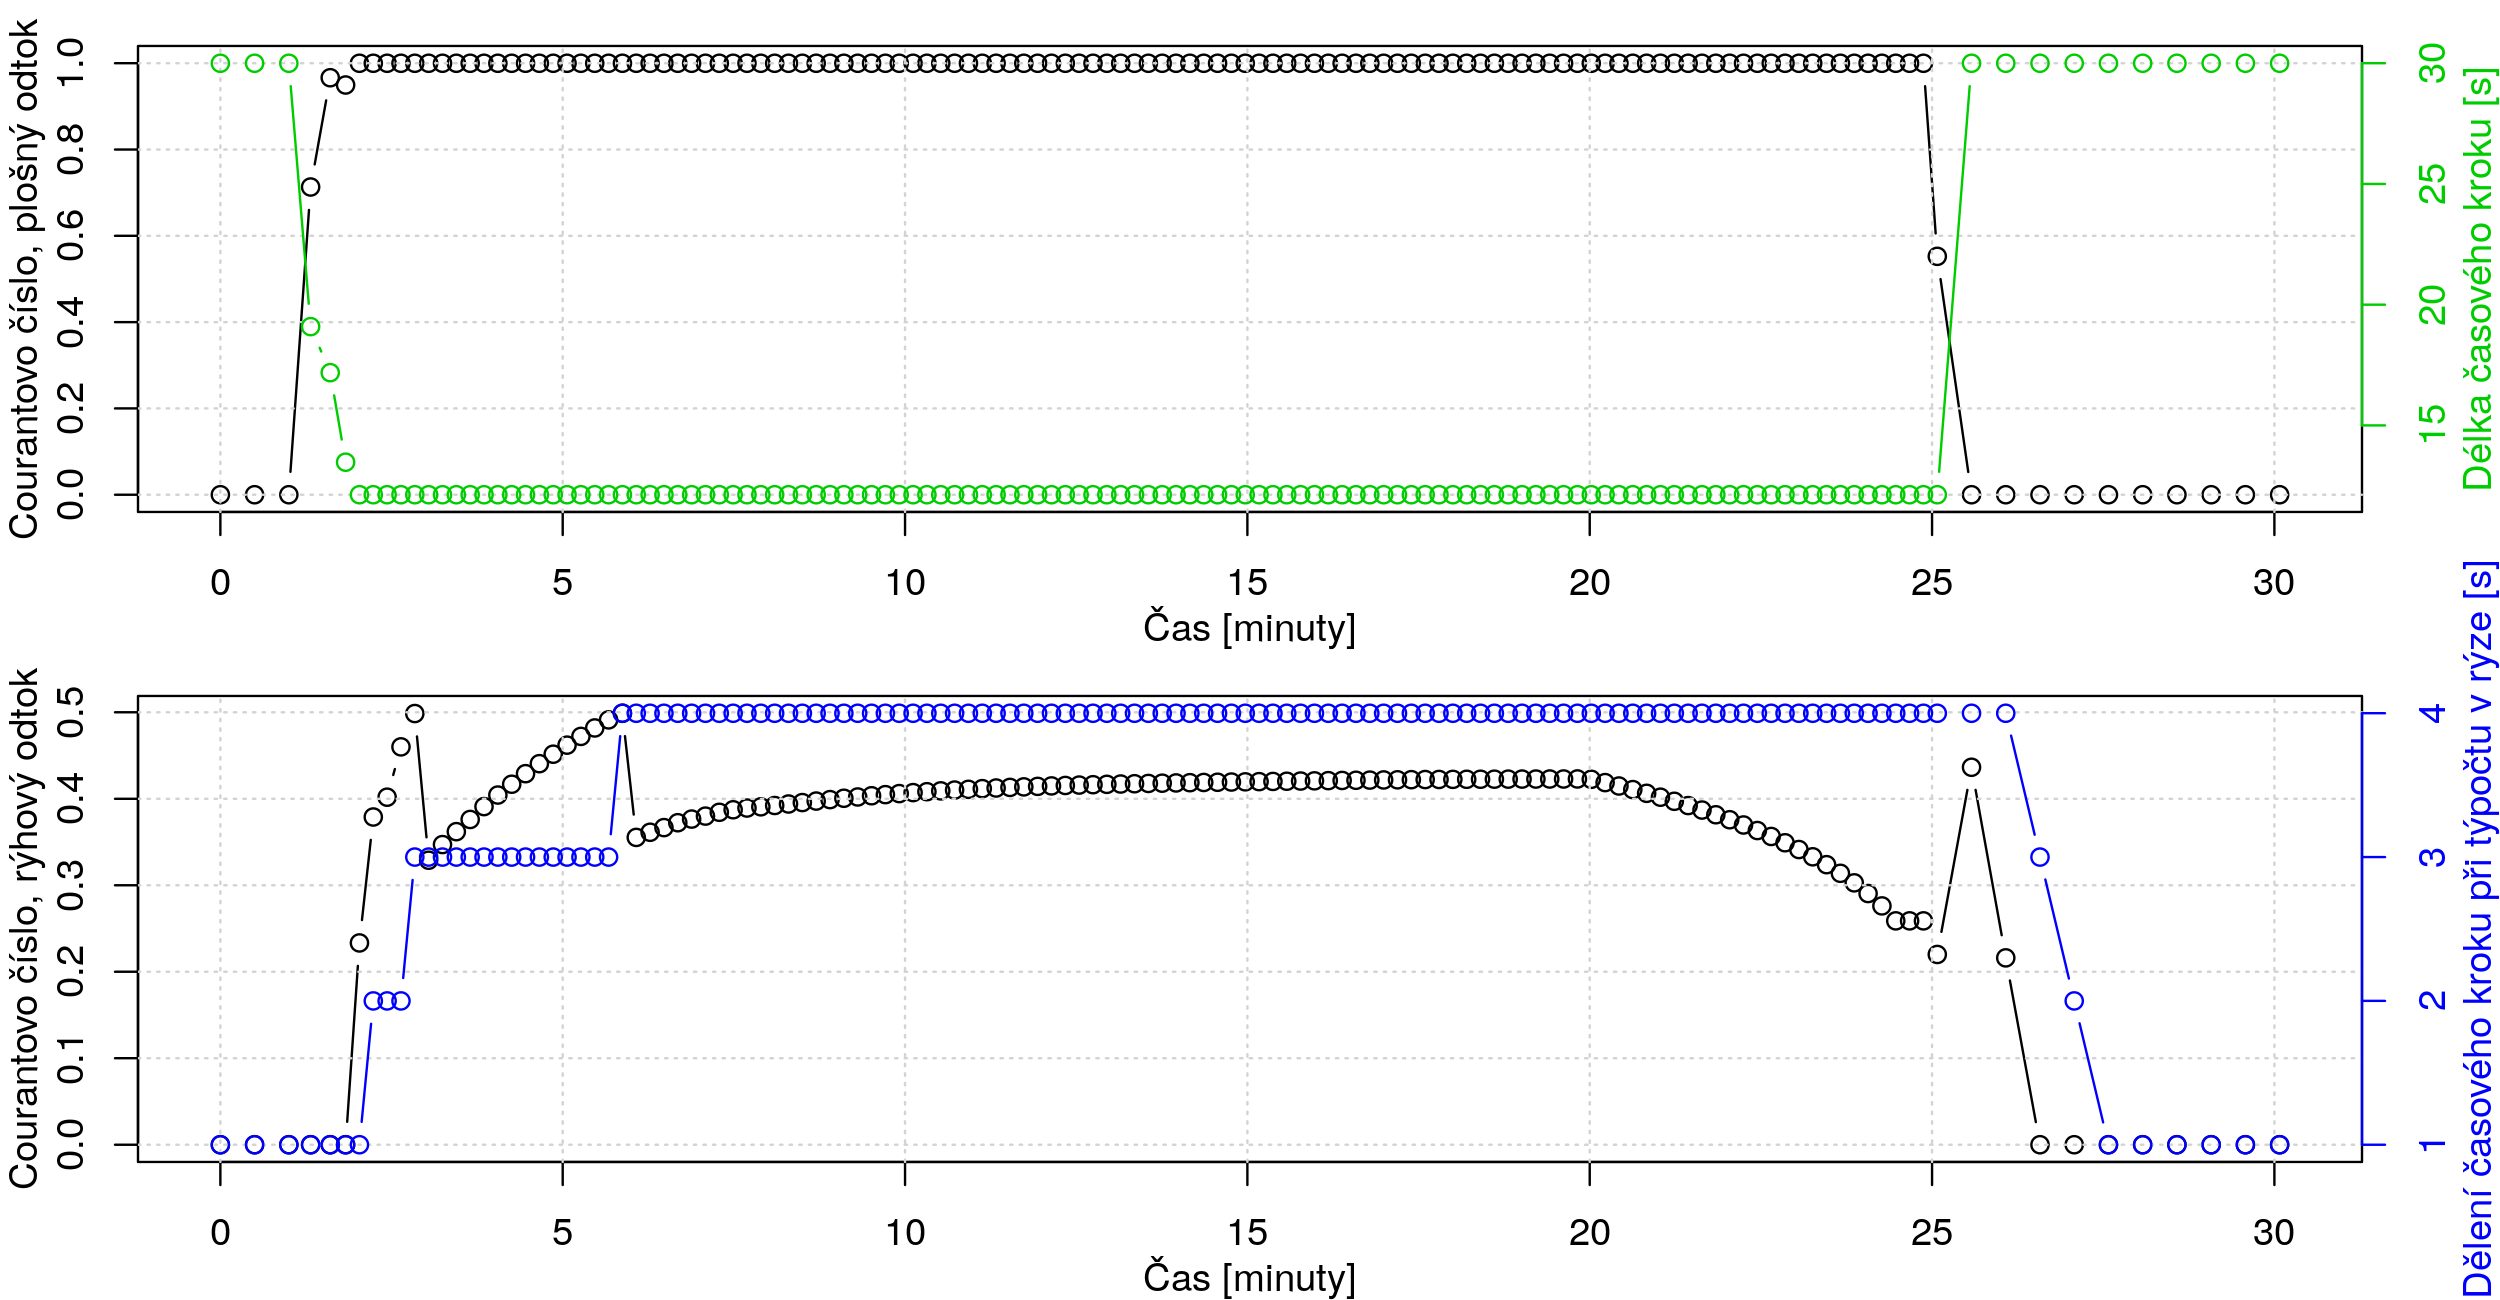
\includegraphics[width=0.8\textwidth]{./img/courantratio.png}
    \caption{Časový krok řízen rychlostí plošného odtoku. \acs{CFL} rychle stoupne k 1 a začne zkracovat časový krok (horní graf). Pár minut později $\acs{CFL}_{rill}$ stoupne nad 0.5, \acs{ratio} stoupne na 2 (dolní graf) tím začne lokálně dělit časový krok při výpočtu rýhového odtoku. \acs{ratio} na spodním grafu stoupne maximální na 4 a neovlivní tedy celkový časový krok (na horním grafu). Na obou grafech je vidět jak se po 25 minutě (kdy v modelu skončila srážková událost) dálka časového kroku i \acs{ratio} vrátí na původní hodnoty.}
    \label{fig:cfl1}
  \end{figure}
%   
%   
  \begin{figure}[p]
    \centering
    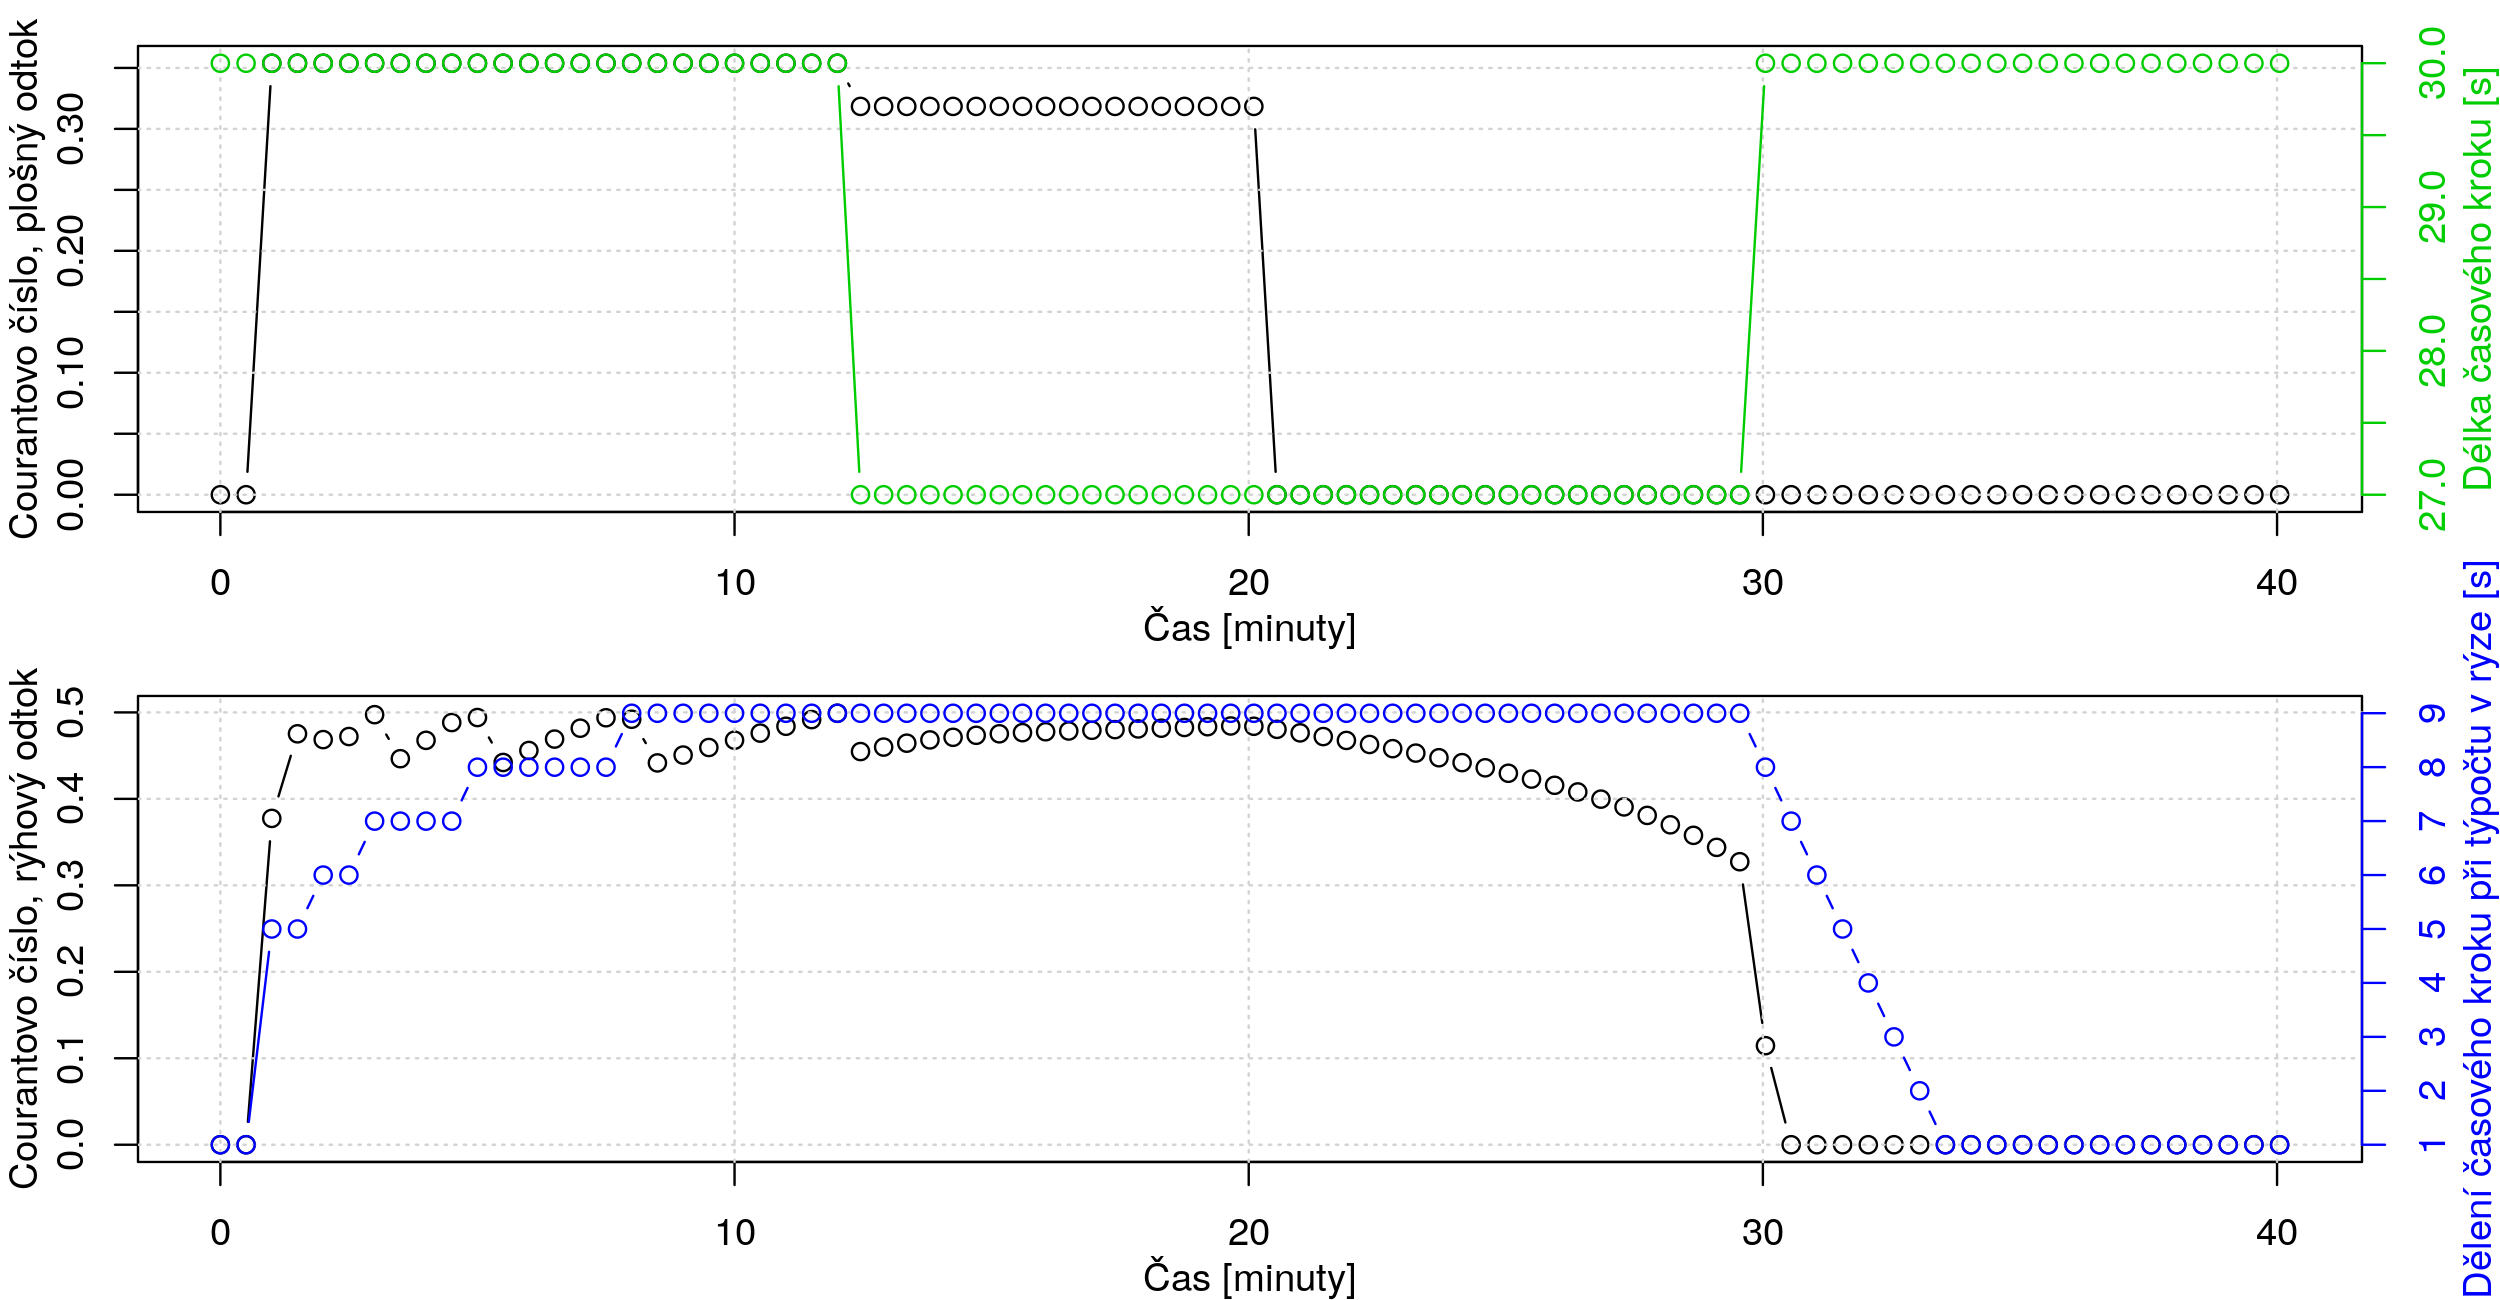
\includegraphics[width=0.8\textwidth]{./img/courantratio2.png}
    \caption{Časový krok řízen rychlostí rýhového odtoku.  \acs{CFL} plošného odtoku nepřekročí během výpočtu hodnotu cca 0.35 (na horním grafu), proto nemá žárný vliv na velikost časového kroku.  $\acs{CFL}_{rill}$ rychle vystoupí 9 krát nad kritickou hodnotu 0.5 (spodní graf, prvních 10 minut výpočtu). To způsobí nárůst \acs{ratio} na 9 což je maximální povolené dělení lokálního časového kroku při výpočtu rýhového odtoku. Pří dalším překročení hodnot 0.3 (cca 12 minuta na dolním grafu) dojde ke zmenšení celkového časového kroku na 90 \% původní hodnoty (horní graf). Na obou grafech je vidět jak se po 20 minutě (kdy v modelu skončila srážková událost) dálka časového kroku i \acs{ratio} vrátí na původní hodnoty.}
    \label{fig:cfl2}
  \end{figure}
  

% Hlavní myšlenkou řešení nestability výpočtu je zmenšení časového kroku při náznaku, že by mohlo dojít k přetečení. Pro každý časový krok je podle rovnice \ref{courrovnice} vypočteno v každé buňce Courantovo číslo $C$. Dále je určeno maximum Courantova čísla ve všech buňkách v časovém kroku. Toto číslo je zásádní, jelikož podle něj se porovnává, zda je situace potencionálně nebezpečná a bude potřeba zmenšit časový krok. Na změnu časového kroku byla použita funkce pojmenovaná $courant$:

% Dochází k porovnání, zda se Courant pohybuje v rozmezí hodnot 0.8 a 1.0. Pokud je hodnota vyšší, je zmenšen časový krok  a pokud je hodnota nižší, časový krok se zvýší. Nikdy však nemůže být výšší než původní časový krok zadaný. Testování probíhalo tak, aby podmínka zmenšila co možná nejméně časový krok a při tom nedošlo k numerické nestabilitě v kroku následujícím. Velikost časového kroku $\Delta t$ zásadně ovlivňuje dobu běhu celého modelu. Čím více se zmenší časový krok, tím déle trvá modelu než doběhne do požadové časové hodnoty a ukončí se. V současné verzi je největším problémem fakt, že při větších průtocích na větším území dojde brzy ke zmenšení $\Delta t$ na velmi nízkou hodnotu, např. 0.01 minuty a tím se úměrně zvyšuje časová náročnost výpočtů.





	
	\section{Výstupy z modelu} \label{kap:vystupy}
	
\pozn{
\textbf{Zde dodelat}
\begin{itemize}
  \item popsat výstupy mimo temp
  \item popsat co jsou v temp
  \item popsat výstupy v určitých krocích
\end{itemize}
}


Výstupy modelu jsou uloženy do složky zadané mezi vstupními parametry (obsah složky je při spuštěné programu vymazán!). Kumulativní nebo maximální hodnoty v jednotlivých  buňkách jsou na konci výpočtu uloženy v rastrovém formátu (viz kapitola~\ref{sec:rastr}). Průnik polygonů prostorové distribuce typu půd a využití území jsou uloženy ve vektorovém formátu (viz kapitola~\ref{sec:vektor}). Pokud model \smod počítá i úseky hydrografické sítě, jsou kumulativní nebo maximální hodnoty veličin jednotlivých úseků vypsáný v atributové tabulce vektorové vrstvy úseků (viz kapitola~\ref{sec:vektor}), prostorové rozložení jednotlivých úseků je uloženo také jako jeden s rastrů (viz kapitola~\ref{sec:rastr}).  Volitelné výstupy hydrogramů  v bodech jsou ve formě časových řad uloženy do textových souborů s příponou {\tt.dat} (viz kapitola~\ref{sec:hydrogramy}).  Jednotlivé výstupy jsou dále popsány podrobněji. 













\subsection{Rastrové výstupy}\label{sec:rastr}

V rastrech jsou uloženy vybrané veličiny jednotlivých buňkách řešeného území. Jako rastrový formát lze zvolit proprietární ESRI formát nebo textový formát ASII. Přehled rastrových výstupních souborů je shrnut v tabulce~\ref{tab:vystupyrast}. Pokud jsou v modelu řešeny i úseky hydrografické sítě jsou buňky rastru ležící na úseku uloženy s hodnotou {\tt NoData} (výjimku tvoří 2 rastry popisující vlastnosti úseků, viz tabulka~\ref{tab:vystupyrast}).  


% jsou ve textovém nebo rastrovém formátu.  








\subsection{Vektorové výstupy}\label{sec:vektor}

Výstupní data modelu ve vektorovém formátu jsou dva. Jedná se topograficky upravenou vrstvu \pozn{topograficka upraha = orientace linie atd...?} úseků hydrografické sítě ({\tt hydReach}), kde jsou do její atributové tabulky doplněny kumulativní a maximální hodnoty vybraných veličin. Tyto veličiny jsou popsány v tabulce~\ref{tab:useky}. Druhým vektorovým výstupem je vrstva, která zobrazuje průnik prostorového rozložení typu půdy a využití území ({\tt interSoilLU}). Ukázka takové vrstvy je na obrázku~\ref{fig:pripravapar_vyrez}d. Tato vektorová vrstva slouží především ke kontrole správnosti přípravy vstupních dat či hledání chyb v nich. 













\subsection{Hydrogramy}\label{sec:hydrogramy}

Pokud jsou do vstupů zadány body pro výpis hydrogramů, vypíší se do testových souborů s příponou {\tt.dat}. Vypsané veličiny jsou závislé na typu odtokového procesu. Popis vypsaných veličin při povrchovém odtoku je shrnut v tabulce~\ref{tab:vystupydat}. Pokud je v buňce úsek hydrografické sítě, vypisují se pouze hodnoty tohoto úseku. Názvy a význam veličin popisující úsek toku jsou popsány v tabulce~\ref{tab:vystupytokdat}. Model v současné verzi uvažuje, že pokud je v buňce úsek hydrografické sítě, zabírá úsek celou buňku, přesto že je jeho šířka menší než šířka samotné buňky.  


% 11.12. Zakomentova radky jsou to tempu


\begin{table}[t]
 

 \centering
 \caption{Přehled rastrových výstupů}
\label{tab:vystupyrast}

% \begin{tabular}{p{4cm}lp{2cm}p{5cm}}
 \begin{tabular}{llp{0.5\textwidth}}
 \hline \hline
  Název souboru    & Jednotka    & Popis       \\ 
  (ESRI nebo .acs)    &     &        \\ \hline 
  cinfilt\_m      &   $m$        & Kumulativní infiltrace \\
  crainf\_m          &  $m$    &  Kumulativní srážka (bez intercepce a povrchové retence) \\
%   csheetvout\_m3      &  $m^3$  & Kumulativní objem odtoku z buňky \\
%   crillvout\_m3       &  $m^3$  & Kumulativní objem odtoku z buňky rýhou \\
  csurvout\_m3       &  $m^3$  & Kumulativní objem odtoku z buňky \\
%   cvin\_m3            &  $m^3$  & Kumulativní objem přítoků do buňky  (plošný + soustředěný) \\
  volrest\_m3          &  $m^3$  & Objem vody zbylé v buňkách po zkončení výpočtu\\
  dmt                 &  $m$ &  Výřez použitého digitálního modelu terénu \\
  flowdir             &  $NA$ &  Rastr s uloženými směry odtoku  \\
  mshearstr\_pa      & $Pa$ &  Maximální tečné napětí \\
%   mreachflm3\_s     &  $m^3s^{-1}$ & Maximální odtok v úsecích hyd. sítě  \\
  msurfl\_m3\_s   &   $m^3s^{-1}$ &  Maximální celkový odtok v buňce\\
  mvel\_m\_s       &   $ms^{-1}$ &  Maximální rychlost proudění v buňce (plošného či soustředěného odtoku) \\
  reachFID            &  $NA$  &  Označuje úseky toku (=fid + 1000), buňky s plošným odtokem (=0) a plošným i soustředěným odtokem (=1) \\
  massbalance         &   $m$  &  Bilance všech vstupů a výstupu z a do buňky  \\
  \hline \hline
%  tyhle jdou do tempu
%  rillAreaM       &   $m^2$      &  Plocha buňky, kterou porývá rýha \\
%  finalCellState    &  $NA$ & Typ odtoku buňky na konci výpočtu (viz sekce~\ref{sec:statpopis})\\
%  critWaterLevelM         & $m$    &  kritický výška hladiny \\
%  mSheetFlowM3_S	  &   $m^3-s^{-1}$	&  Maximální plošný průtok v buňce  \\
%  mRillFlowM3_S    &   $m^3-s^{-1}$	&  Maximální soustředěný průtok v buňce\\
%  mSheetWaterLevelM    &   $m$  &   Maximální výška hladiny plošného v buňce \\
%  mRillWaterLevelM   &   $m$  &   Maximální výška hladiny soustředěného odtoku v buňce \\

 \end{tabular}
 

\end{table}


% cInfiltrationM
% cRainfallM
% cSheetVolOutM3 
% cRillVolOutM3
% cSurfaceVolOutM3
% cVolRestM3
% cReachVolOutM3
% mSurfaceFlowM3_S
% mVelocityM_S
% mReachFlowM3_S
% mShearStressPa
% reachFID
% massBalance





% zakomentovane je do tmp




\begin{table}[h!]
 

 \centering
 \caption{Popis veličin  tabulky úseků hydrografické sítě}
\label{tab:useky}

% \begin{tabular}{p{4cm}lp{2cm}p{5cm}}
 \begin{tabular}{llp{0.5\textwidth}}
  \hline  \hline
 Název sloupce        & Jednotka     & Popis                                 \\ 
 \hline
 FID            &   ---          &  Identifikátor přiřazeného úseku ({\it feature id})   \\
 cVolM3         &  $m^3$         & Kumulativní objem odtoku                              \\
 mFlowM3\_S      &   $m^3s_{-1}$  & Maximální průtok                                      \\
 mFlowTimeS     &   $s$          &  Čas dosažení maximálního průtoku                     \\
 mWatLM         &  $m$       &  Maximální výška hladiny v úseku                               \\
%  mWatLTimeS     &  $s$       &  Čas dosažení maximálního průtoku                              \\
%  cSurInFM3      &  $m^3$     &  Kumulativní přítok do úseku z jeho okolí   \\
 restVolM3      &  $m^3$     &  Objem v úseku po skončení výpočtu         \\
%  cVolDomM3      &  $m^3$     &  Kumulativní odtok úseku z řešeného území (hodnota je nulová pokud úsek odtéká do jiného navazujícího úseku)   \\
 toFID          &  ---       &  FID úseku do které daný úsek odtéká (hodnota -9999 vyjadřuje situaci, kdy úsek kříží hranici řešeného a odtéká tedy mimo toto území) \\
  \hline
   \hline
 \end{tabular}

\end{table}



% FID;V_out_cum [L^3];Q_max [L^3.t^{-1}];timeQ_max[s];h_max [L];timeh_max[s];
% Cumulatice_inflow_from_field[L^3];Left_after_last_time_step[L^3];Out_form_domain[L^3];to_reach



% % zakomentovane je do tmp

\begin{table}[h!]
 

 \centering
 \caption{Popis veličin  v {\tt.dat} souborech}
\label{tab:vystupydat}

% \begin{tabular}{p{4cm}lp{2cm}p{5cm}}
 \begin{tabular}{llp{0.5\textwidth}}
  \hline  \hline
 Název sloupce    & Jednotka    & Popis       \\ 
  \hline
%  \hline
%  Buňka s plošným odtokem:	 &&\\
 time[s]          &   $s$      &  Čas výpočetního kroku          \\
 deltaTime[s]     &   $s$        &  Aktuální délka časového kroku  \\
 rainfall[m]      &  $m$         &  Srážková výška v aktuálním časovém kroku \\
%  sheetWaterLevel[m]       &  $m^3$  & Výška hladiny plošného odtoku \\
%  sheetFlow[m3/s]       &  $m^3s^{-1}$  & Průtok plošného odtoku  \\
%  sheetVolRunoff[m3]    &  $m^3$     & Odteklý objem plošného odtoku \\
%  sheetVolRest[m3]      &  $m^3$     & Objem zbytku vody po plošném odtoku \\
%  infiltration[m]         &  $m$      & Výška infiltrace v daném časovém kroku \\
%  surfaceRetention[m]    &  $m$      & Výška zadržené vody na povrchu v daném časovém kroku \\
%  callState                   &  -         & Typ odtoku na buňce (viz sekce~\ref{sec:statpopis})  \\
%  inflowVol[m3]   &   $m^3$ &  Celkový objem přítoku do buňky \\
 totalWaterLevel[m]	  &   $m$	&  Celková výška hladiny  \\ 
%  \hline
%  Pro soustředěný odtok &&\\ \hline 
%  rillWaterLevel[m]         &   $m$       &  Výška hladiny v buňce se soustředěným odtokem* \\
%  rillWidth[m]	       &   $m$ &  Šířka rýhy vzniklá soustředěným odtokem\\
%  rillFlow[m3/s]      &   $m^3s^{-1}$       &  Průtok v rýze soustředěného odtoku \\
%  rillVolRunoff[m3]   &   $m^3$  &   Objem soustředěného odtoku rýhou \\
%  rillVolRest[m3]  &  $m^3$ &   Objem zbytku vody po soustředěném odtoku rýhou  \\
 surfaceFlow[m3/s]   &  $m^3_{-1}$ & Celkový průtok (plošný + soustředěný)  \\
 surfaceVolRunoff[m3]   &   $m$  & Celkový odteklý objem (plošný + soustředěný) \\
%  rillInflowVol[m3] & $m$ &  @@@ toto tam chcem? to je V\_inflow cast co jde do ryhy, pridal jsem to tam jednou kdyz jsem hledal nejakou chybu...\\
%  ratio & $m$ &  Počet krácení časového kroku v rýhách @@@(je pro nas?)\\
%  sheetCourantCrit & $m$ &  Courantovo kritérium pro plošná odtok @@@(je pro nas?)\\
%  rillCourantCrit & $m$ & Courantovo kritérium pro soustředěný odtok @@@(je pro nas?) \\
%  nIter & $m$ &  Počet iterací pří výpočty daného výpočetního kroku @@@(to bych tam nechal, muže to napověděl jestli se tam neděje něco moc rychle, což může znamenat chybu v zadaných datech, třeba dát 600 mm do srážky místo 60 mm) \\
  \hline
   \hline
   \multicolumn{3}{p{\textwidth}}{*výška hladiny u soustředěného odtoku není výška skutečné výška hladiny v rýze, ale v nadkritická výška hladiny vztažená na celou plochu výpočetní buňky}
 \end{tabular}

\end{table}

% zakomentovane je do tmp

\begin{table}[h!]
 

 \centering
 \caption{Popis veličin  v {\tt.dat} souborech}
\label{tab:vystupydat}

% \begin{tabular}{p{4cm}lp{2cm}p{5cm}}
 \begin{tabular}{llp{0.5\textwidth}}
  \hline  \hline
 Název sloupce    & Jednotka    & Popis       \\ 
  \hline
%  \hline
%  Buňka s plošným odtokem:	 &&\\
 time[s]          &   $s$      &  Čas výpočetního kroku          \\
 deltaTime[s]     &   $s$        &  Aktuální délka časového kroku  \\
 rainfall[m]      &  $m$         &  Srážková výška v aktuálním časovém kroku \\
%  sheetWaterLevel[m]       &  $m^3$  & Výška hladiny plošného odtoku \\
%  sheetFlow[m3/s]       &  $m^3s^{-1}$  & Průtok plošného odtoku  \\
%  sheetVolRunoff[m3]    &  $m^3$     & Odteklý objem plošného odtoku \\
%  sheetVolRest[m3]      &  $m^3$     & Objem zbytku vody po plošném odtoku \\
%  infiltration[m]         &  $m$      & Výška infiltrace v daném časovém kroku \\
%  surfaceRetention[m]    &  $m$      & Výška zadržené vody na povrchu v daném časovém kroku \\
%  callState                   &  -         & Typ odtoku na buňce (viz sekce~\ref{sec:statpopis})  \\
%  inflowVol[m3]   &   $m^3$ &  Celkový objem přítoku do buňky \\
 totalWaterLevel[m]	  &   $m$	&  Celková výška hladiny  \\ 
%  \hline
%  Pro soustředěný odtok &&\\ \hline 
%  rillWaterLevel[m]         &   $m$       &  Výška hladiny v buňce se soustředěným odtokem* \\
%  rillWidth[m]	       &   $m$ &  Šířka rýhy vzniklá soustředěným odtokem\\
%  rillFlow[m3/s]      &   $m^3s^{-1}$       &  Průtok v rýze soustředěného odtoku \\
%  rillVolRunoff[m3]   &   $m^3$  &   Objem soustředěného odtoku rýhou \\
%  rillVolRest[m3]  &  $m^3$ &   Objem zbytku vody po soustředěném odtoku rýhou  \\
 surfaceFlow[m3/s]   &  $m^3_{-1}$ & Celkový průtok (plošný + soustředěný)  \\
 surfaceVolRunoff[m3]   &   $m$  & Celkový odteklý objem (plošný + soustředěný) \\
%  rillInflowVol[m3] & $m$ &  @@@ toto tam chcem? to je V\_inflow cast co jde do ryhy, pridal jsem to tam jednou kdyz jsem hledal nejakou chybu...\\
%  ratio & $m$ &  Počet krácení časového kroku v rýhách @@@(je pro nas?)\\
%  sheetCourantCrit & $m$ &  Courantovo kritérium pro plošná odtok @@@(je pro nas?)\\
%  rillCourantCrit & $m$ & Courantovo kritérium pro soustředěný odtok @@@(je pro nas?) \\
%  nIter & $m$ &  Počet iterací pří výpočty daného výpočetního kroku @@@(to bych tam nechal, muže to napověděl jestli se tam neděje něco moc rychle, což může znamenat chybu v zadaných datech, třeba dát 600 mm do srážky místo 60 mm) \\
  \hline
   \hline
   \multicolumn{3}{p{\textwidth}}{*výška hladiny u soustředěného odtoku není výška skutečné výška hladiny v rýze, ale v nadkritická výška hladiny vztažená na celou plochu výpočetní buňky}
 \end{tabular}

\end{table}


% % zakomentovane je do tmp



\begin{table}[h!]
 

 \centering
 \caption{Popis veličin  v {\tt.dat} souborech}
\label{tab:vystupytokdat}

% \begin{tabular}{p{4cm}lp{2cm}p{5cm}}
 \begin{tabular}{llp{0.5\textwidth}}
  \hline  \hline
 Název sloupce        & Jednotka     & Popis                                      \\ 
 \hline
 time[s]              &   $s$         &  Čas výpočetního kroku                    \\
 deltaTime[s]         &   $s$         &  Aktuální délka časového kroku            \\
 rainfall[m]          &  $m$          &  Srážková výška v aktuálním časovém kroku \\
 reachWaterLevel[m]        &  $m$          &  Výška hladiny plošného odtoku            \\
 reachFlow[m3/s]              &  $m^3s^{-1}$  &  Průtok plošného odtoku                   \\
 reachVolRunoff[m3]                  &  $m^3$     & Odteklý objem plošného odtoku     \\
%  reachVolInflow[m3]              &  $m^3$     & Suma přítoků z okolních buněk úseku v daném časovém kroku \\
%  reachVolRest[m3]         &  $m^3$     & Objem v úseku toku po odtoku      \\
  \hline
 \end{tabular}

\end{table}

% # Time[s];deltaTime[s];Rainfall[m];Waterlevel[m];V_runoff[m3];Q[m3/s];V_from_field[m3];V_rests_in_stream[m3]
% 
% 
% time[s]
% deltaTime[s]
% rainfall[m]
% reachWaterLevel[m]
% reachFlow[m3/s]
% reachVolRunoff[m3/s]
% reachVolInflow[m3]
% reachVolRest[m]
% zakomentovane je do tmp



\begin{table}[h!]
 

 \centering
 \caption{Popis veličin  v {\tt.dat} souborech}
\label{tab:vystupytokdat}

% \begin{tabular}{p{4cm}lp{2cm}p{5cm}}
 \begin{tabular}{llp{0.5\textwidth}}
  \hline  \hline
 Název sloupce        & Jednotka     & Popis                                      \\ 
 \hline
 time[s]              &   $s$         &  Čas výpočetního kroku                    \\
 deltaTime[s]         &   $s$         &  Aktuální délka časového kroku            \\
 rainfall[m]          &  $m$          &  Srážková výška v aktuálním časovém kroku \\
 reachWaterLevel[m]        &  $m$          &  Výška hladiny plošného odtoku            \\
 reachFlow[m3/s]              &  $m^3s^{-1}$  &  Průtok plošného odtoku                   \\
 reachVolRunoff[m3]                  &  $m^3$     & Odteklý objem plošného odtoku     \\
%  reachVolInflow[m3]              &  $m^3$     & Suma přítoků z okolních buněk úseku v daném časovém kroku \\
%  reachVolRest[m3]         &  $m^3$     & Objem v úseku toku po odtoku      \\
  \hline
 \end{tabular}

\end{table}

% # Time[s];deltaTime[s];Rainfall[m];Waterlevel[m];V_runoff[m3];Q[m3/s];V_from_field[m3];V_rests_in_stream[m3]
% 
% 
% time[s]
% deltaTime[s]
% rainfall[m]
% reachWaterLevel[m]
% reachFlow[m3/s]
% reachVolRunoff[m3/s]
% reachVolInflow[m3]
% reachVolRest[m]











% \subsection{State - typ průtoku na buňce}\label{sec:statpopis}
%   Jak bylo popsání no v kapitole~\ref{kap:tok} v modelu je možné řešit několik typů povrchového odtoku: plošný odtok, soustředěný odtoku a odtok hydrografickou sítí. Topografie hydrografické sítě je definována uživatelem. Vznik soustředěného odtoku je podmíněn překročením kritické výšky (popsáno v kapitole~\ref{sec:soustredenyodtok}). V programu jsou typy odtoku rozlišeny celočíselným identifikátorem označeným State, kde pokud State\\
% %   
%   \begin{tabular}{rcl}
%      =     &0&  dochází v buňce pouze k plošnému odtoku pokud \\
%      =     &1&  dochází v buňce k plošnému i soustředěnému odtoku  nebo pokud \\
%      =     &2&  @@@ plošný odtoku a rýha jen odtéká \\
%      && je to v teto verzi? Je to zajímavé pro uživatele? \\
%      $>$=  &1000&  je v buňce úsek hydrografické sítě. \\
%   \end{tabular}
% 
%   Identifikátor hydrografické sítě nemusí začínat číslem 1000 a nemusí být vzestupný (sestupný) u navazujících úseků. Tento identifikátor je v modelu definován jako 1000 + {\tt fid}, je tedy definován uživatelem nebo přiřazen použitým GIS softwarem. 
% 









%\section{Výstupní data} \label{section:vystupnidata}

%Po úspěšném ukončení modelu je do výstupního adresáře uloženo několik souborů. Každý z těchto souborů obsahuje hodnoty pro každou buňku rastru. Buňky, na kterých neprobíhal výpočet neobsahují žádné hodnoty, tedy NoData. Základní výstupy jsou uvedeny přímo ve zvoleném výstupním adresáři. Mimo hlavní výstupy jsou volitelně ukládány i dočasné výstupy sloužící pro případnou kontrolu. V podadresáři \textbf{temp} jsou dočasné soubory výpočtu v ploše a v podadresáři \textbf{temp_dp} jsou dočasné soubory vodních toků. \textbf{Dočasným výsledkům bude věnována jedna z dalších kapitol}







\textbf{toto je origoš z DP}

\par Ne vždy se vytvoří všechny tyto výstupní soubory. Záleží na zvolených vstupních parametrech. Pokud uživatel nezadá žádnou bodovou vrstvu, nevytvoří se poslední textový soubor. 
V případě, že uživatel nezvolí možnost soustředěného odtoku, nevytvoří se rastry a shapefile související s tímto typem odtoku. Rastr soustředění odtoku se nevytvoří při nezvolení vícesměrného odtoku. 
Ostatní soubory se vytvoří pokaždé.  

\textbf{ z diplomky}

Výstupy se ukládají do adresáře nazvaného output. Cestu k němu si volí uživatel v rámci vstupních dat (viz kap. 2.3.1). Model prochází stále vývojem a dotýká se to i výstupních souborů. Princip ale zůstává stejný a jedná se spíše o úpravy zdrojového kódu zajištující lepší přehlednost a práci s kódem pro budoucí úpravy. Např. práce s vícerozměrnými maticemi a převedení všech výpočtů do základních (SI) jednotek. 
Výsledkem modelu jsou soubory (.shp, .rst, .txt, .dbf), které reprezentují parametry (Zajíček J., 2014):
hladina
Výstupem jsou hodnoty maximální výšky hladiny pro každou buňku. Jedná se tedy o rastrovou vrstvu vytvořenou porovnáváním hodnot výšek hladiny v každém časovém kroku. Uložena je nejvyšší hodnota. Výška hladiny v jednotlivých krocích je získána pomocí bilance přítoků a odtoků do buňky.  
průtok
Výstupem jsou hodnoty maximálního průtoku pro každou buňku. Obdobně jako u hladiny jsou porovnávány hodnoty v jednotlivých krocích a uložena maximální hodnota. Hodnoty průtoku v jednotlivých časových krocích jsou vypočteny pomocí metody kinematické vlny (teorie viz kap. 1.5.2).
infiltrace
Výstupem infiltrace jsou hodnoty v každé buňce, které jsou během doby běhu modelu postupně načítány až do vyčerpání infiltrační kapacity.
zbytkový objem
Zbytkovým objemem se rozumí objem, který v dané buňce v časovém kroku zůstal. V případě odtoku veškeré vody z rastru je rastr nulový. Matematicky je objem vyjádřen jako rozdíl celkového objemu v buňce (zbytkový objem z předchozího kroku a přítoky) a povrchového a soustředěného odtoku.
odtok
Výstup týkající se odtoku slouží pro konečnou bilanci (kontrolu) a testování. Jedná se o celkové množství, které z buňky odteklo za celou dobu běhu modelu. 
rychlost
Rastr rychlostí je výstupem sloužící k určení erozní ohroženosti. Porovnávány jsou hodnoty skutečných rychlostí s limitními nevymílacími rychlostmi (viz tab. č. 3 ).
napětí. 

Obdobou je rastr tečného napětí. Slouží k určení míst potencionálně nebezpečných. Hodnoty limitních hodnot tečného napětí jsou uvedeny ve stejné tabulce jako rychlosti průtok v rýze (viz tab. č. 3 ).

Průtok v rýze je rastrová vrstva znázorňující maximální průtok v rýze při soustředěném odtoku. Výstup je vytvořen jen při volbě typu výpočtu s uvažováním rýhového odtoku. Rýha vznikne pouze v buňkách, kde výška hladiny překročí hladinu kritickou. 
rychlost v rýze
Rastr obsahuje hodnoty maximální rychlosti v buňkách, kde je rýha vytvořena. Výpočet v rýhách probíhá odlišně oproti povrchovému odtoku. Jedná se o větší rychlosti, a proto na těchto buňkách probíhá výpočet za běžný časový krok 3x. V jiném případě by hrozilo, že výpočet nebude konvergovat.
souhrn

Final evalution.txt je textový soubor, který obsahuje souhrn zadaných vstupů a čas běhu modelu a bilanci vody. 
hydrogram
Point hydrographs.txt je textový soubor s hodnotami výšky hladiny, průtoku, napětí, rychlostí v bodech zadaných vstupní bodovou vrstvou. Soubor slouží k tvorbě hydrogramů v těchto bodech. Automaticky je k vrstvě přidán bod, ve kterém je hodnota flow acumulation nejvyšší.
Výstupem v současnosti je i řada dalších vrstev, které slouží ale spíše k tvorbě a testování modelu a pro samotného uživatele nejsou potřebné.	

}





%\clearpage
%\newpage\null\thispagestyle{empty}\newpage


  \newpage
  \part{Ukázka výsledků}
%   %!TEX ROOT = ../mainCZ.tex
%\input{./1_text/3_mat_a_met/2}

Úvodní část je věnována historickému pozadí a vývoji modelu SMODERP. Odvození parametrů o kterých se hovoří v kapitole \ref{SM_hist} jsou podrobně popsány v kapitole \ref{Exp_mer}. Použité fyzikální vztahy jsou popsány v kapitole \ref{modelovani}. SOučasná verze modelu z hlediska zpracování vstupních dat, výpočtu a uváděných výstupů je pak v kapitole \ref{vypocet}.


\setcounter{section}{0}
\section{Porovnání metod 1D a 2D} \label{porovnani1D2D}
\setcounter{section}{0}
\section{Porovnání metod 1D a 2D} \label{porovnani1D2D}


1D and 2D approaches which are subject to comparison were designated by a hydrograph and runoff volume in the breach profile. The respective comparison was carried out on two locations in the Czech Republic (Hořanský stream and Býkovický catchment). A system of erosion control measures was implemented in this area. The size of the given area being subject to this research is 1.5 $ km^{2} $. For 1D model are the individual agricultural plots were distinguished by 12 different profiles.

\begin{figure}[ht!]
\centering
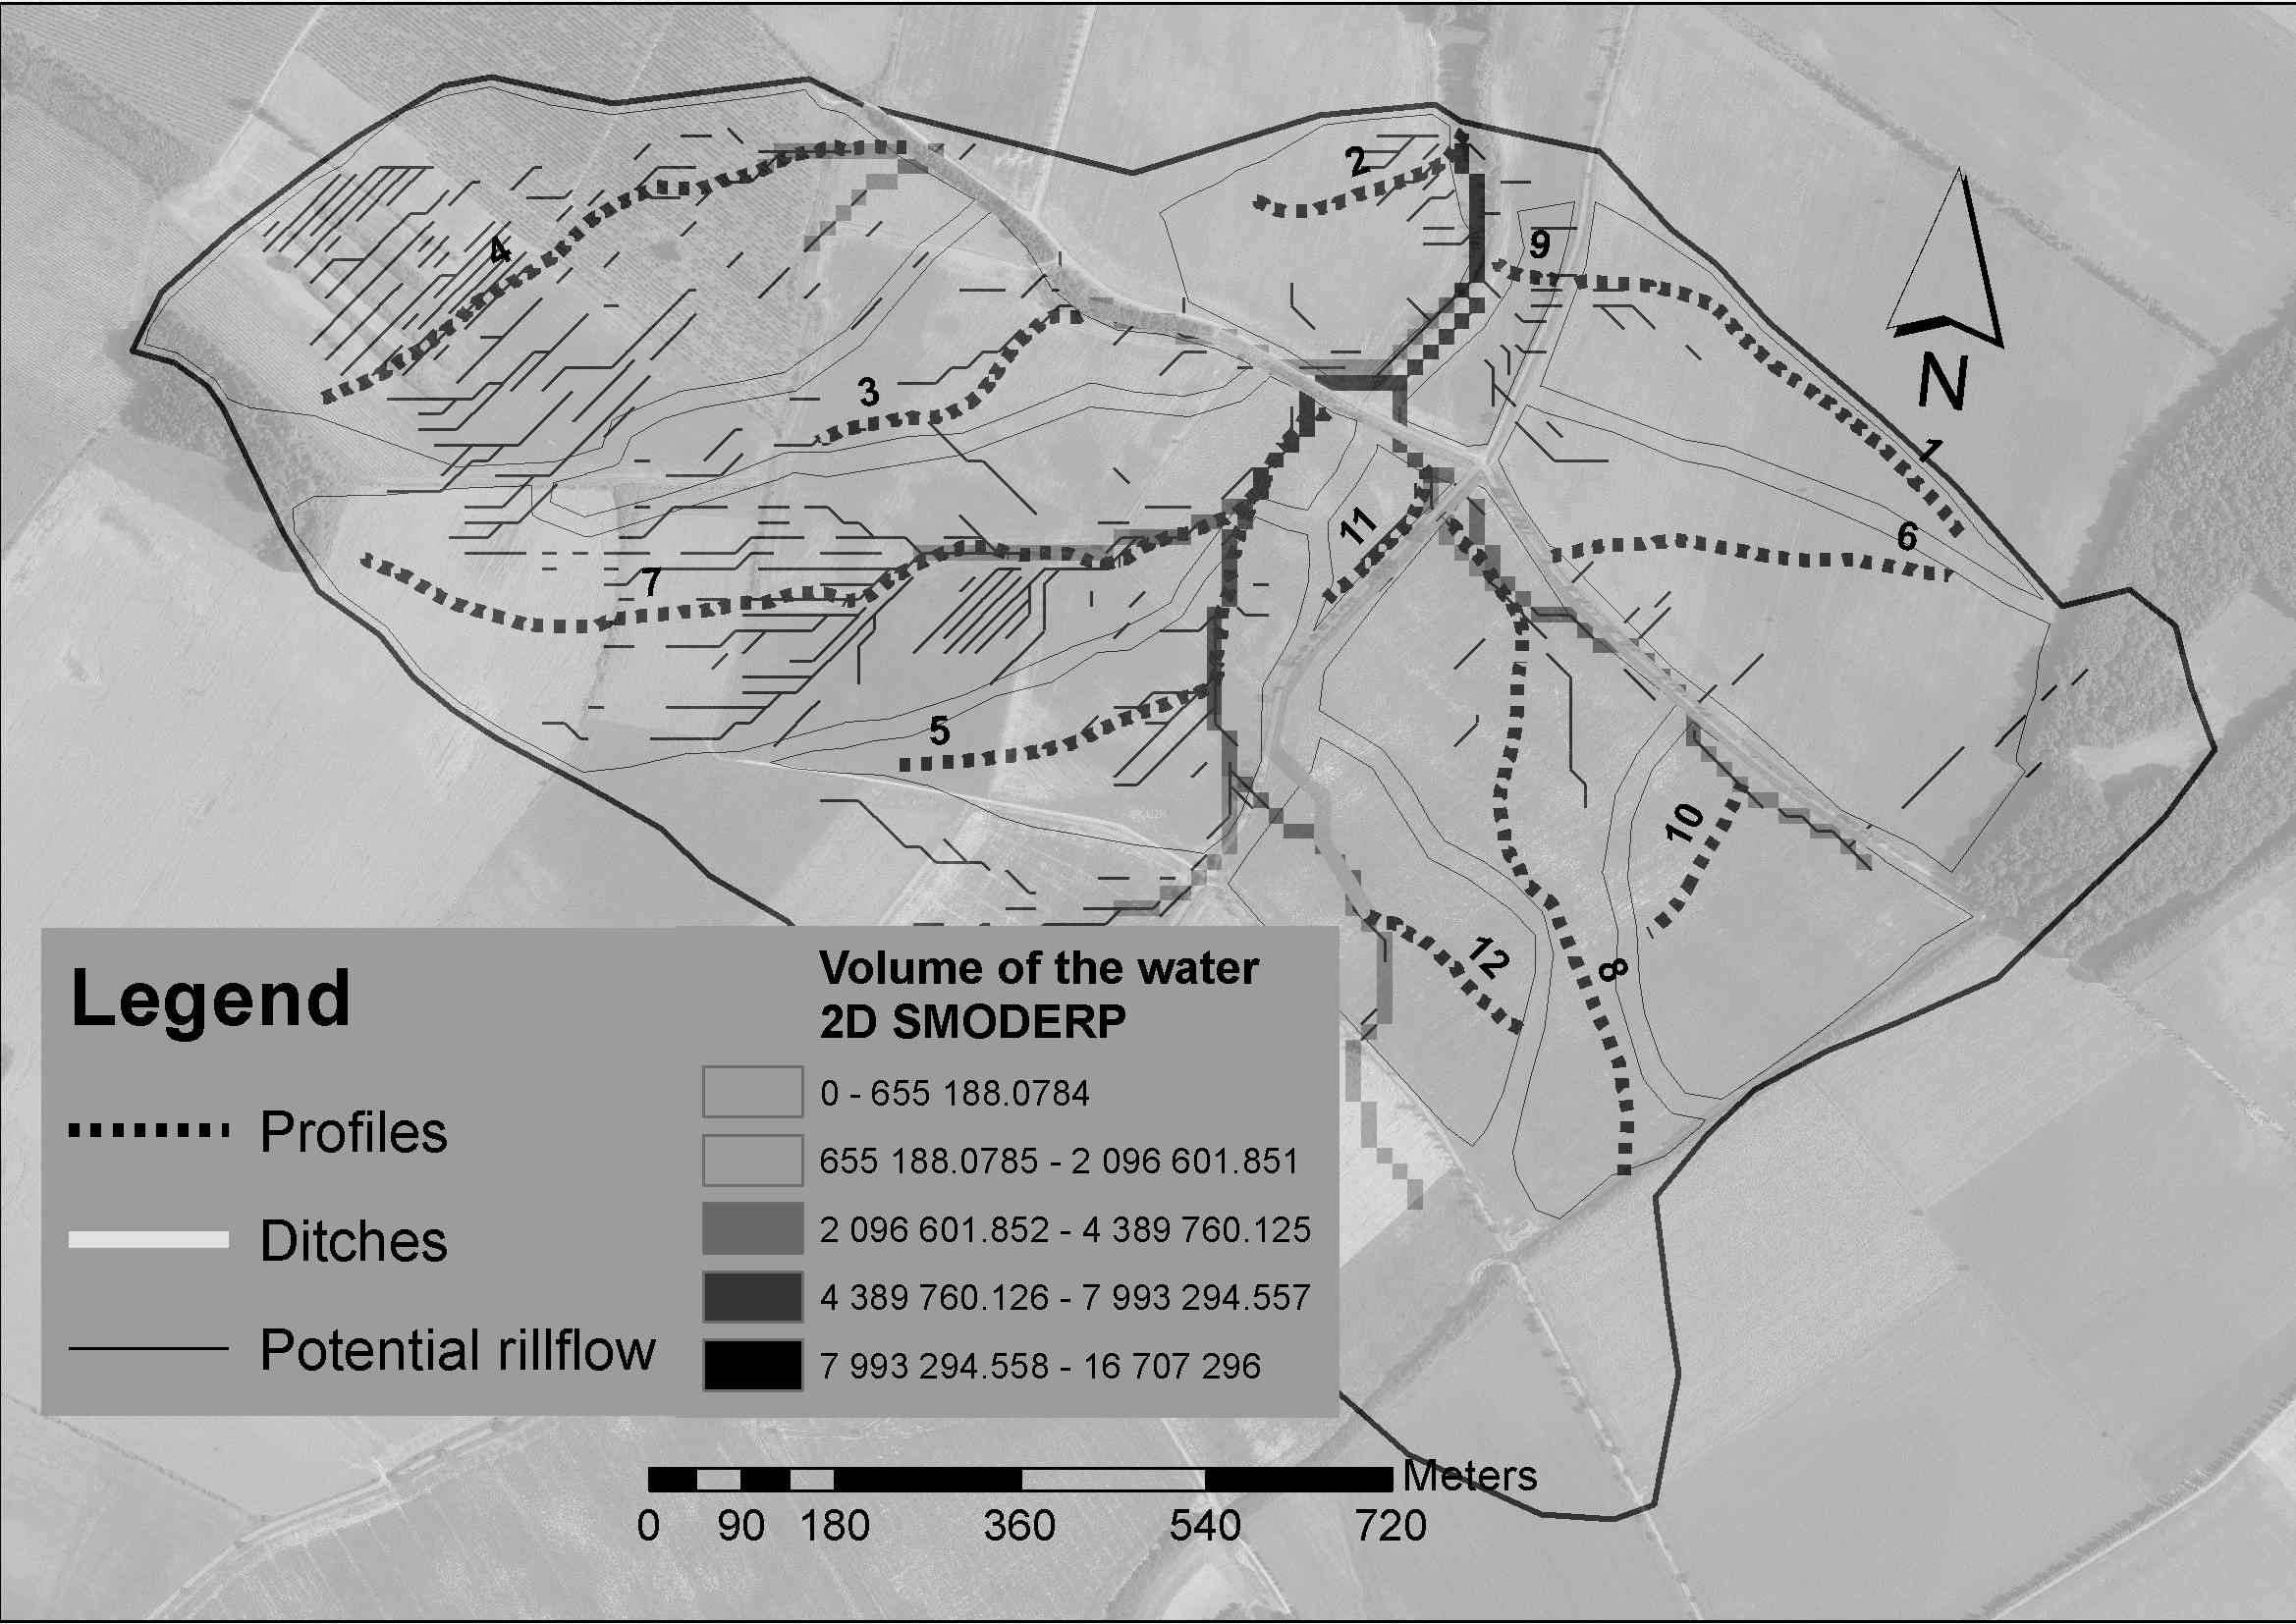
\includegraphics[width=0.8\textwidth]{img/horany_print3.jpg}
\caption{Profiles and runof concetration - Horany}
\label{fig:horany}
\end{figure}\FloatBarrier

\begin{figure}[ht!]
\renewcommand{\figurename}{Graf}
\centering
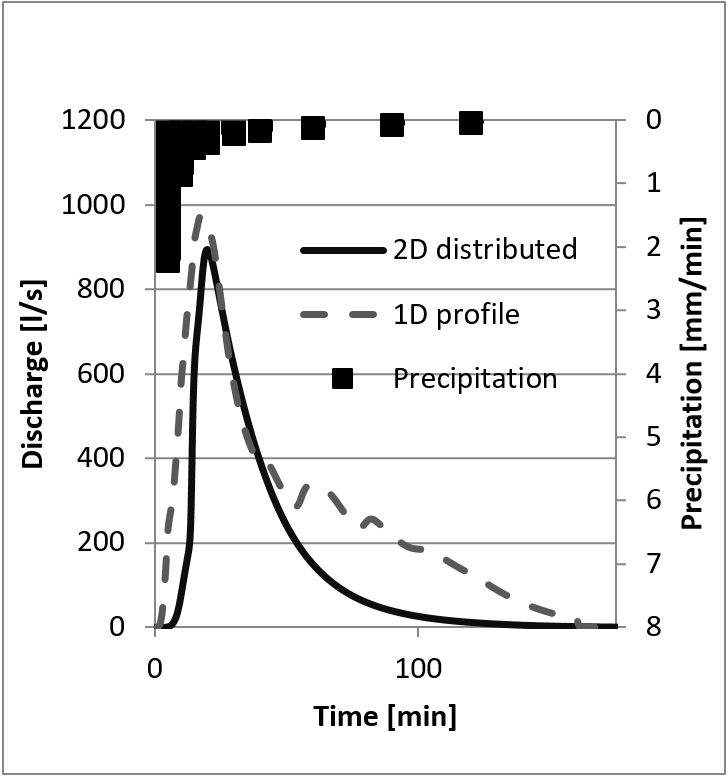
\includegraphics[width=0.8\textwidth]{graph/1D2Dhorany.png}
\caption{Hydrographs 1D and 2D Smoderp - Horany study area}
\label{graf:graf_1}
\end{figure}\FloatBarrier

The second location is formed by the independent agricultural plot situated in the Býkovický potok basin (Benešov u Prahy) with a morphologically distinctive lane of concentration runoff. Experimental measurements of erosion processes were carried out on the given plot for a considerable period of time. It is thus possible to compare the final results for the appropriate model with measured values. Six characteristic profiles were created on the given plot (size of ten acres). This number exceeds considerably the amount of profiles which were necessary for the description of the given small area. The number of profiles was appointed in order to make comparisons between 1D and 2D approaches, as well as from the reasons explaining the influence of a large number of profiles on the final characteristics. Standardized field erosion plots were installed and situated on a farmer plot in the surveyed area for monitoring the overland flow and sediment transport. The resulting cooperation between the 1D and 2D approaches was executed during the real rainstorm with measured surface runoff.

\begin{figure}[ht!]
\centering
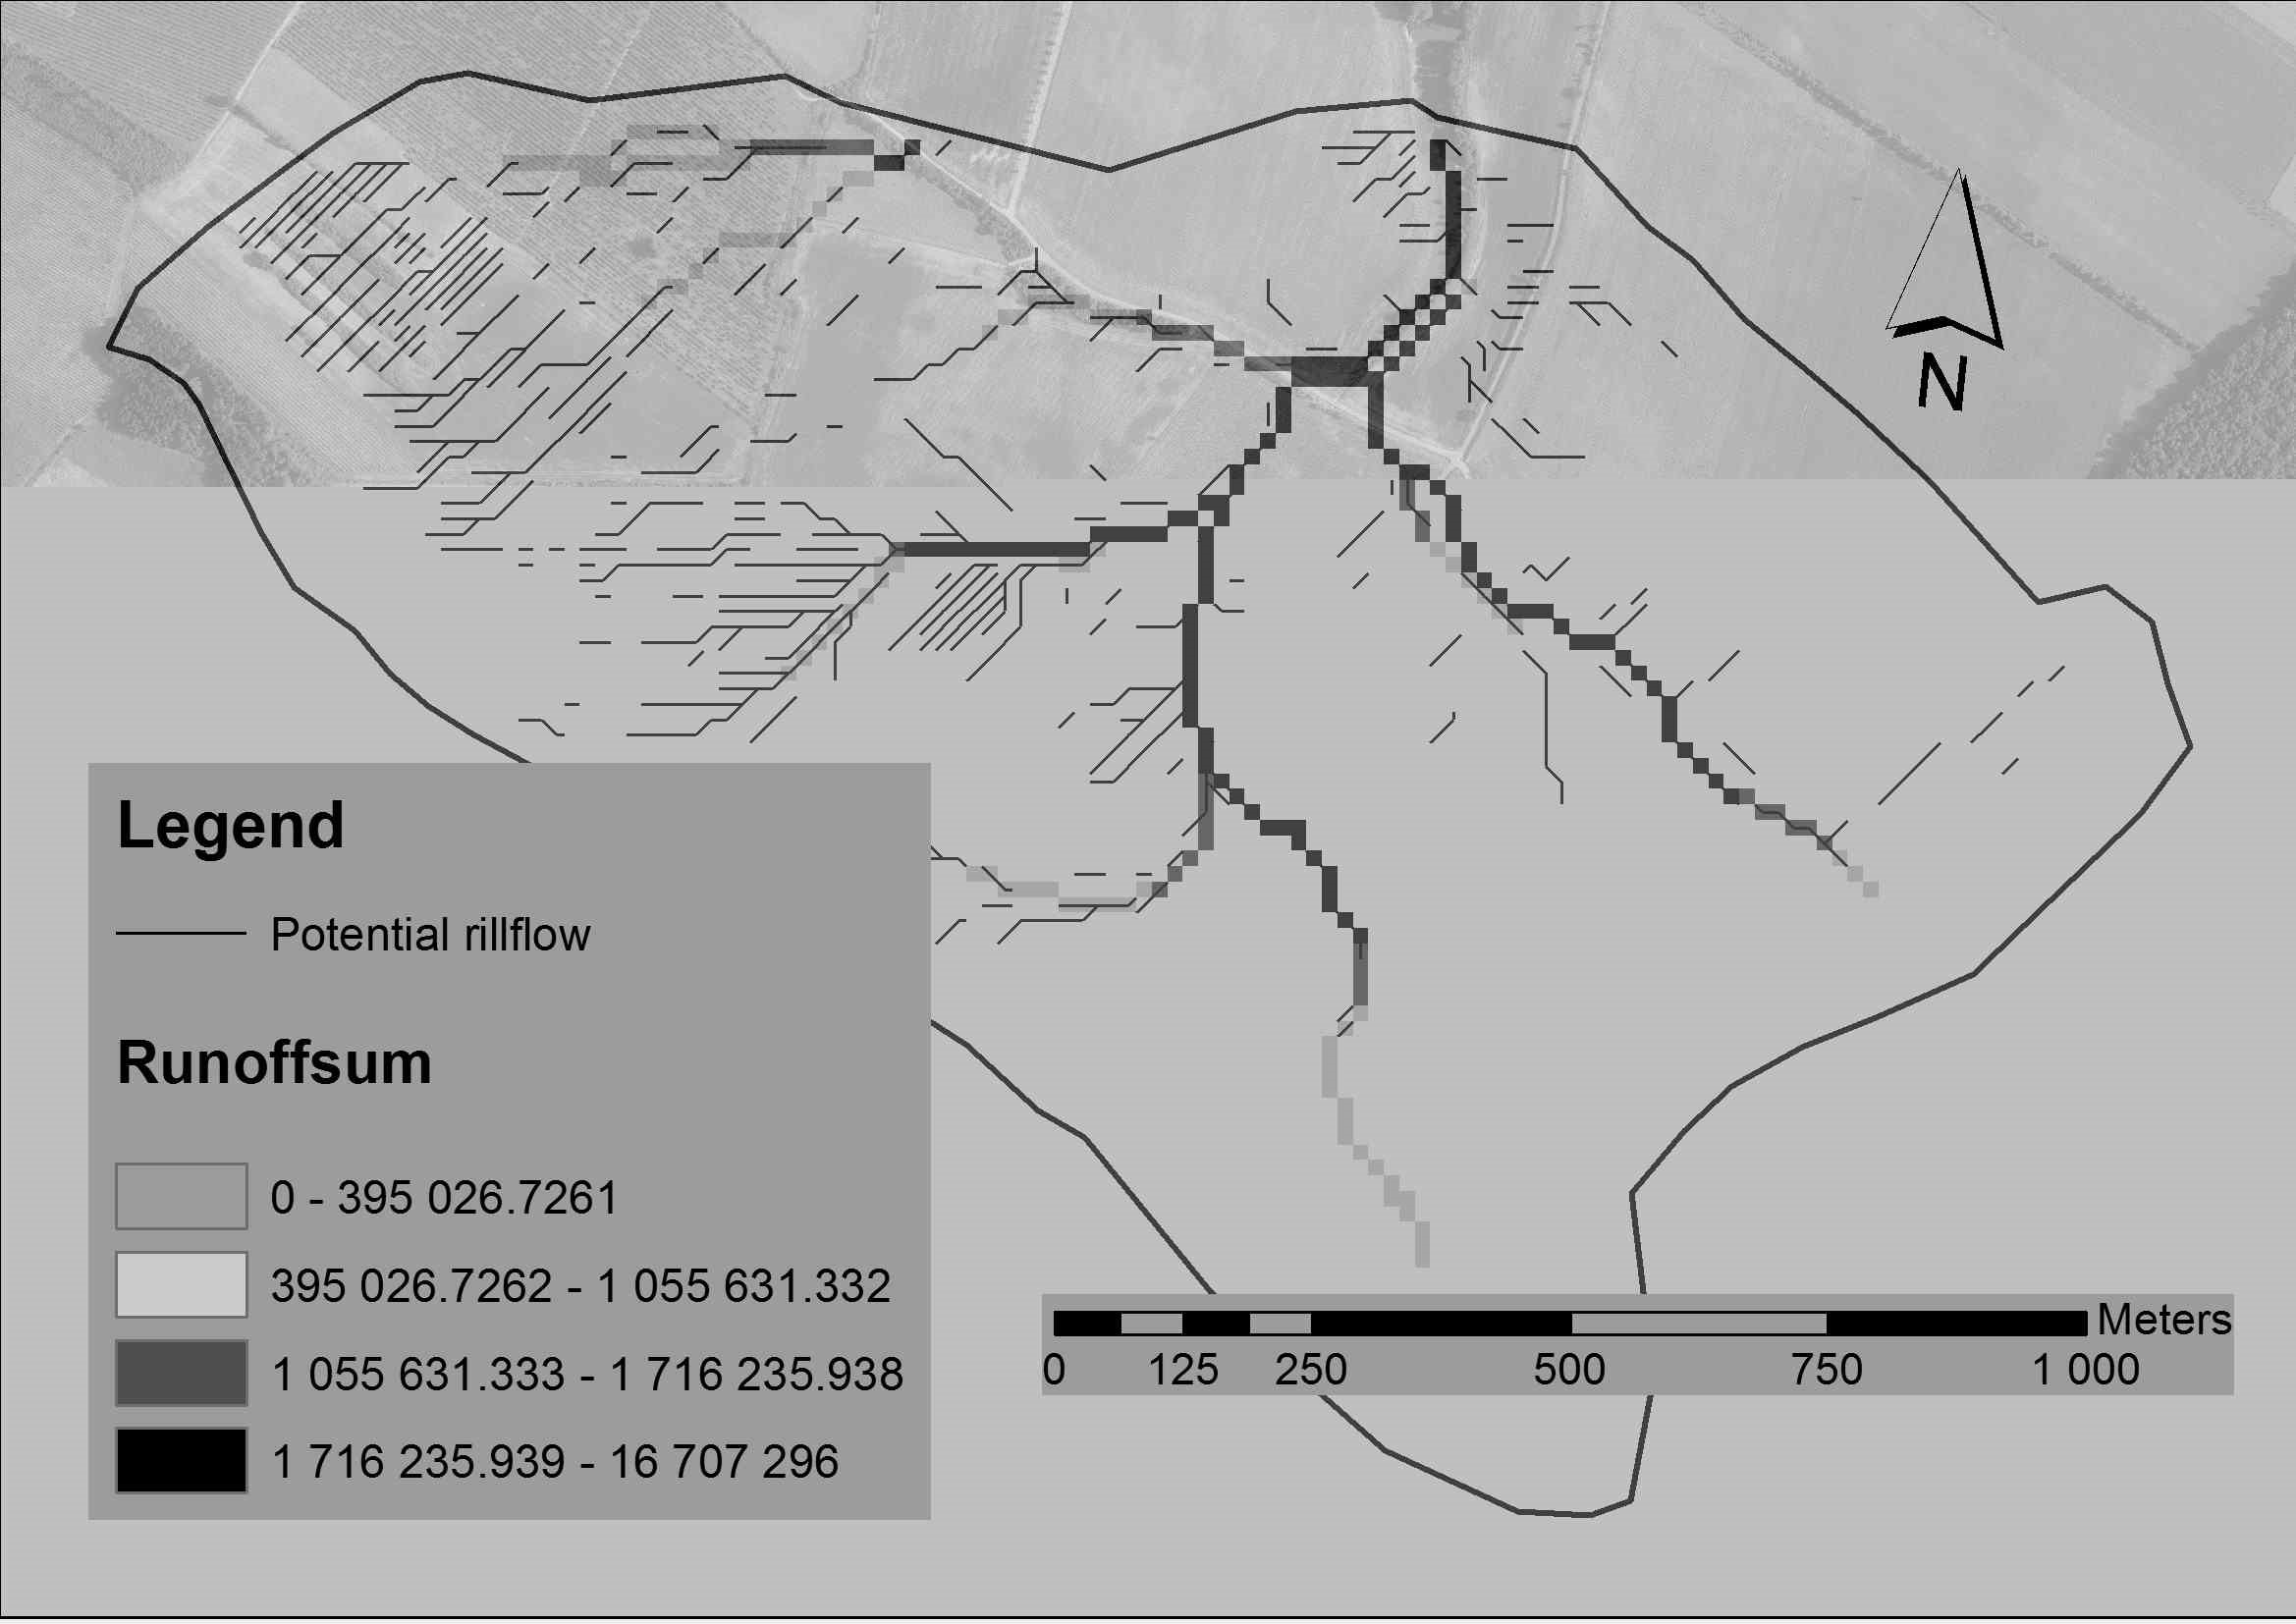
\includegraphics[width=0.8\textwidth]{img/byk.jpg}
\caption{Profiles and runof concetration - Bykovicky catchment }
\label{fig:horany}
\end{figure}\FloatBarrier

\begin{figure}[ht!]
\renewcommand{\figurename}{Graf}
\centering
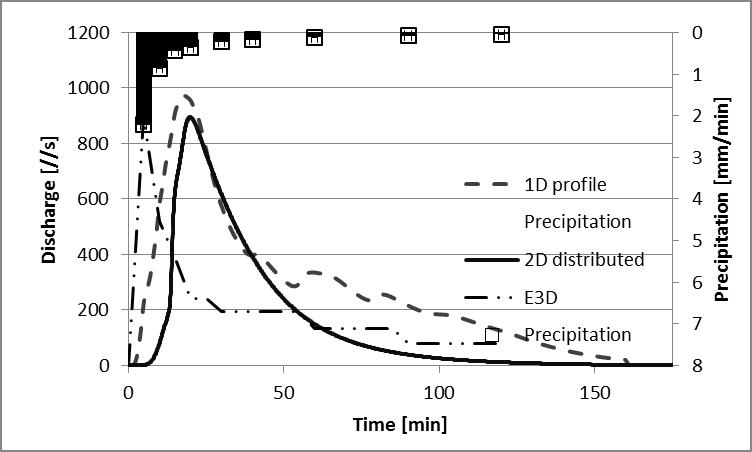
\includegraphics[width=0.8\textwidth]{graph/1D2DByk.jpg}
\caption{Hydrographs 1D and 2D Smoderp - Bykovicky catchment}
\label{graf:graf_1}
\end{figure}\FloatBarrier

The results based on hydrograph measurements taken from individual profiles in both locations were progressively added to the breach profile (outlet). In order to compare the discharge process, the values of surface level, discharge and a cell of the breach profile were extracted in the 2D model version for testing. The implementation of this process is enabled in the development environment of the particular model.

%\clearpage
%\newpage\null\thispagestyle{empty}\newpage

  % %!TEX ROOT = ../mainCZ.tex
%\input{./1_text/3_mat_a_met/2}

První část manuálu popisuje jednotlivé výpočetní vztahy použité v modelu \smod. Základní odvození povrchových procesů v modelu \smod vychází z rovnice kontinuity a pohybové rovnice. Pohybová rovnice je zjednodušená pomocí teorie kinematické vlny. Tímto způsobem je tok řízen mocninný vztahem, jehož parametry byly měřeny (viz  příloha~\ref{sec:priloha}). 

Jak již bylo zmíněno v úvodu, model \smod je distribuovaný epizodní hydrologicko-erozní model. Výpočet je řešen na pravidelné rastrové síti. Prostorová diskretizace modelu je řízena  rozlišením vstupního digitálního modelu terénu. V celém řešeném prostoru je po jednotlivých buňkách v každém časovém kroku provedena bilance vstupů a výstupů a následně vypočteno odteklé množství v daném časovém úseku v buňce. Formálně se jedná o řešení metodou konečných diferencí s explicitně řešenou časovou diskretizací. V bilanční rovnici jsou řešeny tři základní složky:


\begin{itemize}\itemsep 0cm
\item infiltrace do půdy \acs{Inf},
\item efektivní srážka \acs{ES},
\item přiteklé a odteklé množství \acs{Itot} a \acs{Otot}.
\end{itemize}


Odteklé množství může být dále složeno ze tří základních typů odtoku: \textbf{plošného} povrchového odtoku, \textbf{soustředěného rýhového} povrchového odtoku a odtoku dočasnou \textbf{hydrografickou sítí} (tok otevřeným korytem). V ploše povodí jsou směry odtoků odvozeny na zahladě odtokových algoritmů. V místě úseků hydrografické sítě je veškerý tok směrován touto sítí.\\
% PeKa - pokuso jsem se rozdělit povrchový odtok (plošný a rýhy dohromady), ab bylo jasnější o co jde
% 
% 
\rule{\textwidth}{0.3pt}
% % % % %	\subsubsection{Použité rovnice}
%%!TEX ROOT = ../mainCZ.tex
% 
% 
% 
%
% Plošný povrchový odtok
%
%
%
Základní odvození vztahů povrchových procesů v modelu SMODERP vychází z rovnice kontinuity a rovnice pohybové na základě kinematického principu s využitím experimentálních měření.
Jak již bylo zmíněno v úvodu, jedná se o distribuovaný epizodní hydrologicko erozní model. Výpočet je řešen na pravidelné rastrové síti elementů. Podrobnost řešení je dána rozlišením vstupního rastru. V celém řešeném prostou je po jednotlivých elementech v každém časovém kroku provedena bilance zásoby a následně vypočteno odteklého množství za daný časový krok. Obecně se jedná o tři základní složky:

\begin{itemize}
\item infiltrace do půdy\acs{Inf}
\item efektivní srážka \acs{ES}
\item odteklé množství \acs{Otot}
\end{itemize}

Proudění povrchové vody a množství odtoku je pak podle řešeno třemi odlišnými typy odtoku:
\begin{itemize}
\item plošný odtok
\item soustředěný odtok v rýhách
\item výpočet odtoku v hydrografické síti
\end{itemize}

V ploše povodí jsou směry odtoků resp. přítoků dány funkcí směru odtoku. V místě vodních toků je pak veškerý tok směrován dále vodním tokem.


\subsubsection{Plošný povrchový odtok} 

% 
% 
% 
% 
Základním vztahem řešení v elementu je bilance plošného odtoku.
\begin{equation}
\acs{dS} = \acs{Itot} - \acs{Otot},
\label{eq:bilobecne}
\end{equation}
% 
% 
% 
% kde se aktuální změna  zásoby $S$ rovná rozdílu sumy aktuálních přítoků  \acs{Itot} a sumy aktuálních odtoků \acs{Otot}.
\begin{tabular}{rrl}
  kde \jj{dS}{,}
      \jj{Itot}{,}
      \jj{Otot}{.}
\end{tabular}




Podle složek povrchového odtoku lze \acs{Itot} a \acs{Otot} rovnici~\ref{eq:bilobecne}  rozepsat takto podle složek povrchového odtoku použitých v modelu SMODERP 




$$
  \acs{Itot} = \acs{ES} + \acs{Oin},
$$
$$
  \acs{Otot} = \acs{Inf} + \acs{Oout},
$$
% 
% kde \acs{Oin} je přítok ze sousední výpočetní buňky (buněk) a \acs{Oout} je odtok z dané buňky. 
\begin{tabular}{rrl}
  kde \jj{Oin}{,}
      \jj{Oout}{,}
      \jj{ES}{,}      
      \jj{Inf}{.}
\end{tabular}


Bilanční rovnici pro každou buňku $i$ v čase $t$ lze rozepsat jako




\begin{equation} 
\frac{\mathrm{d}S}{\mathrm{d}t} = \acs{ES}_{i,t} + \sum_j^m \acs{Oin}_{j,t-1} - \acs{Inf}_{i,t} - \acs{Oout}_{i,t-1},
\label{eq:bilancnirceV}
\end{equation}
% 
% 
% 
% kde $m$ jsou buňky, odkud vtéká voda do buňky $i$. 
\begin{tabular}{rrl}
  kde & $m$ & jsou buňky, odkud vtéká voda do buňky $i$. 
\end{tabular}


Toto $m$ se liší podle použitého odtokového algoritmu jednosměrného \acs{D8} nebo vícesměrného \acs{mfda} ({\it multi-flow direction algorithm}). Objem srážky \acs{ES} a infiltrované množství \acs{Inf} lze určit přímo při výpočtu časového kroku $t$. Přiteklé a odteklé množství vody \acs{Oin} a \acs{Oout} z časového kroku $t-1$ (což odpovídá explicitnímu řešení časové derivace). 




Při samotném řešení se v modelu SMODERP operuje s veličinami ve výškových jednotkách. Pokud celou rovnici~\ref{eq:bilancnirceV} podělíme velkostí buňky \acs{bunka} a vyjádříme časovou derivaci jako diferenci ($\frac{\mathrm{d}\acs{hsur}_{i,t}}{\mathrm{d}t} \approx \frac{\acs{hsur}_{i,t} - \acs{hsur}_{i,t-1}}{\acs{dT}}$), vypadá rovnice~\ref{eq:bilancnirceV} následovně:




\begin{equation} 
\acs{hsur}_{i,t} = \acs{hsur}_{i,t-1} + \acs{dT}\left(\acs{es}_{i,t} + \sum_j^m \acs{oin}_{j,t-1} - \acs{inf}_{i,t} - \acs{oout}_{i,t-1}\right),
\label{eq:bilancnirce}
\end{equation}
% 
% 
% 
% 
% kde \acs{hsur} je výška hladiny na povrchu, \acs{es} je intenzita srářky, \acs{inf} je intenzita infiltrace, \acs{oin}(\acs{oout}) odteklá (přiteklá) výška za čas. 
\begin{tabular}{rrl}
  kde \jj{hsur}{,}
      \jj{es}{,}
      \jj{inf}{,}
      \jj{oin}{,}
      \jj{oout}{.}
\end{tabular}
% 
% 
\\ V následujícím textu jsou popsány jednotlivé členy za pravé straně rovnice~\ref{eq:bilancnirce}.


% 
% 
% 
% 
% 
% 
% Efektivní srážka \acs{ES}
% 
% 
% 
% 
% 
% 
% 
\paragraph{Efektivní srážka \acs{es}} 

Srážka je příčinou celého erozního procesu. Vzhledem k tomu, že se jedná o epizodní model je srážka zadávána v podobě konkrétní nebo návrhové srážky, která začíná s prvním časovým krokem výpočtu. Model počítá s vlivem intercepce, tedy že určitá část srážky bude zachycena rostlinami díky potenciální intercepci \acs{PotI}. Míra zachycení v každém výpočtovém čase je definována  pomocí poměrné plochy listové \acs{Lai} například \cite{Nevim}.

Označme množství srážky který dopadá na povrch půdy i plodiny během \acs{dT} potenciální srážkou \acs{PS}. Část \acs{PS}, která zůstane v časovém kroku na rostlinách se dá vyjádřit jako násobek srážky \acs{PS} a \acs{Lai},
$$
\acs{PS}\ I_{LAI}
$$
% 
Z tohoto vztahu vyplývá, že množství které propadne povrchem listů je 
$$
\acs{PS}(1 - I_{LAI}).
$$

V modelu je rovněž zahrnuta intercepční kapacita \acs{PotI}, která se plní na začátku běhu modelu. Výsledná intenzita efektivní srážky v čase $t$ je par určena jako
$$
 \acs{es}_t = MAX(0;\sum_{\bar{t} = t_{init}}^{t}\left(\acs{PS}_{\bar{t}}(1 - I_{LAI})\right)-\acs{PotI}))/\acs{dT},
$$
% kde suma $\sum_{\bar{t} = t_{init}}^{t}$ vyjadřuje množství srážky které propadlo povrchem listů plodiny od počátečního času $t_{init}$ do času $t$.
\begin{tabular}{rrl}
  kde \jj{PS}{,}
      \jj{Lai}{,}
      \jj{PotI}{\ a}
      & $\sum_{\bar{t} = t_{init}}^{t}$ & vyjadřuje množství srážky které propadlo \\
      && povrchem listů plodiny od počátečního času $t_{init}$ do času $t$.
\end{tabular}



% 
% 
% 
% 
% 
% 
% 
% 
% 
% 
\paragraph{Intenzita infiltrace \acs{inf}}

V modelu je použita infiltrace podle Philipa \citep{philip1957} v~následujícím tvaru (pro příslušnou buňku $i$):
\begin{eqnarray} \label{eq:phillip}
\acs{inf} = \frac{1}{2}\acs{Sorb}t^{-1/2}+\acs{Ki}.
\end{eqnarray}
% 
% 
\begin{tabular}{rrl}
  kde \jj{inf}{,}
      \jj{Sorb}{\ a}
      \jj{Ki}{.}
\end{tabular}




Philipova rovnice byla zvolena především z důvodu relativně malého počtu nutných vstupních parametrů. tato zjednodušená rovnice má dva hlavní členy nasycenou hydraulickou vodivost \acs{K} a sorbtivitu \acs{Sorb}. Autoři modelu si byli vědomi omezení použití Philipovy rovnice vyplývající z podmínek, za kterých byla odvozena.  Možné odchylky způsobené volbou této rovnice odpovídají odchylkám v heterogenitě půdy a kvalitě ostatních vstupů, na jejichž základě model pracuje. Čas $t$ ve vztahu~\ref{eq:phillip} je čas od začátku srážky, který by měl být v epizodním modelu totožný s počátečním časem výpočtu. Tato nezbytná podmínka by měla být brána v potaz při přípravě vstupních dat. 
% 
% 
% 
% 
% 
% 
% 
% 
% 
% 
% 
\paragraph{Plošný odtok  \acs{oin}, \acs{oout}} \label{rce_odtok}
Rovnice plošného odtoku vychází z kinematického přístupu k řešení pohybové rovnice,
% 
% 
% 
$$
  \acs{qsur} = \acs{a}\acs{hsur}^{\acs{b}},
$$
% 
% 
% 
\begin{tabular}{rrl}
  kde \jj{qsur}{,}
      \jj{a}{\ ($a = \acs{X}\acs{I}^{\acs{Y}}$)\ a}
      \jj{b}{.}
\end{tabular}




Parametry \acs{a} a \acs{b} respektive \acs{X} a \acs{Y} jsou odvozeny na základě měření, viz kapitola \ref{Exp_mer}. Z vyhodnocení vyplývá, že parametr b je závislý pouze na půdním druhu. Parametr a je závislý nejen na půdním druhu, ale také na sklonu svahu. Odteklá resp. přitelká výška je pak dopočítána jako



$$
   \acs{oout} (resp.\ \acs{oin}) = \frac{\acs{dX}}{\acs{bunka}}\acs{qsur}
$$
%
% 
\begin{tabular}{rrl}
  kde \jj{dX}{\ a}
      \jj{bunka}{.}
\end{tabular}

% $$
% q_{sur} [m^{3}/s] = Ah_{sur}^{b} \Rightarrow \frac {1}{n} a h_{sur}^{X} i_{0}^{Y}
% $$

\textbf{ověřit sklon v\%}

% 
% 
% 
% 
% 
% 
% 
% 
% 
% 
% 
% 

\paragraph{Odvozené veličiny}

Z vypočteného průtoku, velikosti řešeného elementu a délky časového lze dopočítat objem odtoku
$$
  \acs{Vout} = \acs{dT}\acs{qsur},
$$
% 
% 
% 
% 
\begin{tabular}{rrl}
  kde \jj{Vout}{.}
\end{tabular}




Pro posouzení erozní ohroženosti a pro výpočet vzniku rýh je v každém elementu vypočítávána rychlost a tečné napětí. Za předpokladu, že se jedná a proudění vody o malé hloubce, lze rychlost proudění odvodit ze specifického průtoku a výšky hladiny:
% 
% 
% 
% 
% 
\begin{equation}
  \acs{vsur} =  \frac{\acs{qsur}}{\acs{hsur}},
  \label{eg:v}
\end{equation}
% 
% 
% 
\begin{tabular}{rrl}
  kde \jj{vsur}{.}
\end{tabular}




Tečné napětí dále využívané v modelu pak uvažuje výpočet tak, jak jej uvádí například \citep{Schwab1993}
% 
% 
% 
\begin{equation}
\acs{tau} = \acs{ro} \acs{g} \acs{hsur} \acs{I}\acs{K} \label{eg:tau},
\end{equation}
% 
% 
% 
\begin{tabular}{rrl}
  kde \jj{tau}{,}
      \jj{ro}{,}
      \jj{g}{,}
      \jj{I}{\ a}
      \jj{K}{.}
\end{tabular}



Vypočítaná rychlost a tečné napětí jsou v případě posuzování erozní ohroženosti porovnávány s limitními hodnotami krajních nevymílajících rychlostí a tečnéch napětí pro jednotlivé půdní druhy v závislosti na druhu vegetace \citep{DyrovaE.1984} a jsou uvedeny v tabulce 
\ref{tabulkaDyrova}. % tabulka neni 
V literatuře se setkáme i s odlišnými hodnotami. Například M. A. Velikanov stanovil krajní nevymílající rychlost pro půdy 0,24 $m/s$  \citep{CabikJ.1963}, což je hodnota nižší, než kterou stanovila E. Dýrová.


% 
% 
% 
% 
% 
% 
% 
% 
% 
% 
% 
\subsubsection{Soustředěný odtok v rýhách} \label{sec:soustredenyodtok}

Výpočet soustředěného odtoku v rýhách implementovaný do modelu SMODERP vychází z několika předpokladů:
\begin{enumerate}
  \item Zavedení stejných zjednodušujících předpokladů výpočtu proudění obdobně jako v~případě výpočtu plošného odtoku, přesto že se nejednáo výpočet proudění o zanedbatelně malé hloubce. Předpokladem je, že se v jednotlivých elemetech v relativně malých časových krocích jedná o rovnoměrné ustálené proudění. Při rovnoměrném proudění se předpokládá sklon dna \acs{I} rovný sklonu hladiny vody v rýze a shodná drsnost v celé délce elementu. Průtok v rýze je vyjádřen použitím Chézyho rovnice v mannigově tvaru:
  \begin{equation}
    \acs{qrill} = \acs{vrill} \acs{A} = \acs{A} \frac{1}{\acs{n}} \acs{Rrill}^{2/3} \acs{I}^{1/2}  ,
    \label{eq:qrill}
  \end{equation}
  \begin{tabular}{rrl}
    kde \jj{qrill}{,}
        \jj{vrill}{,}
        \jj{A}{,}
        \jj{n}{\ a}
        \jj{Rrill}{.}
  \end{tabular}

  
  
  \item Soustředěný odtok vniká v elementech, kde dojde k překročení kritické hladiny \acs{hcrit}, která je spočtena pro každý element na základě  hodnot kritického tečného napětí \ref{eg:tau} nebo rychlostí \ref{eg:v}. Objem vzniklé rýhy odpovídá nadkritickému množství vody \acs{Vrill}.
  $$
  \acs{Vrill}= \acs{Vtot} - \acs{Vcrit} = MAX(0;\acs{hsur} - \acs{hcrit}) \acs{bunka}
  $$
  \begin{tabular}{rrl}
    kde \jj{Vrill}{,}
        \jj{Vtot}{,}
        \jj{Vcrit}{\ a}
        \jj{hcrit}{.}
  \end{tabular}
  

  \item Další z důležitých zjednodušení je tvar příčného profilu rýhy, který je v modelu reprezentován obdélníkem, s pevným poměrem stran \acs{rratio}=výška/šířka rýhy. Velikost rýhy se zvětšuje pokud je nadkritické množství \acs{Vrill} větší než objem samotné rýhy. Pak se výška rýhy rovná výšce vodní hladiny v rýze (vlevo na obrázku~\ref{fig:rill_schema}). Pokud začne být nadkritické množství \acs{Vrill} menší než je velikost rýhy, začne se rýha prázdnit, velkost rýhy však zůstává konstantní (vpravo na obrázku~\ref{fig:rill_schema}). Hydraulický poloměr rýhy lze určit podle následujícího vztahu
%   
% 
% 
%   Rozměry rýhy nejsou známy, protože rozměr rýhy \acs{hrill}, \acs{brill} se dynamicky mění v závislosti na množství vody během simulace. 
%   
  \begin{figure}
    \centering
    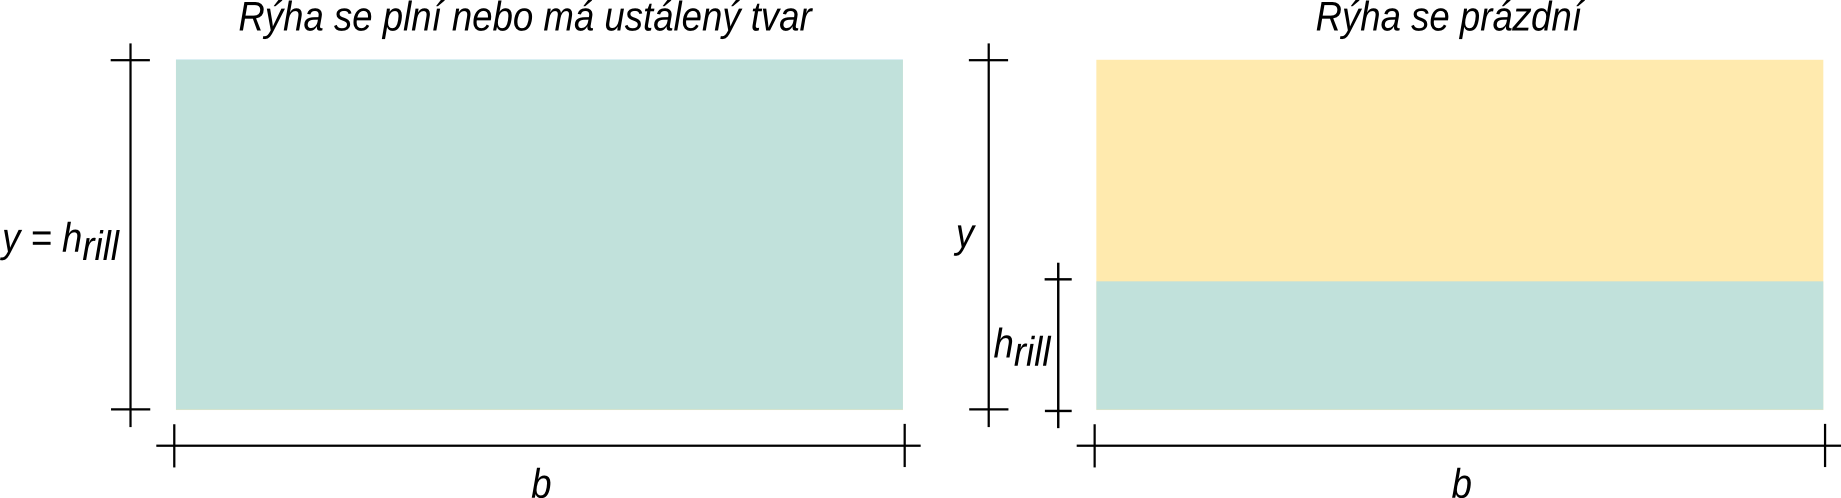
\includegraphics[width=0.9\textwidth]{./img/rill_schema.png}
    \caption{Tvar rýny a výška vodní hladiny při plnění rýny či ustálení proudění (napravo), tvar rýny při jejím prázdnění (nalevo)}
    \label{fig:rill_schema}
  \end{figure}
% 
%   
  $$ 
    \acs{Rrill} = \frac{\acs{A}}{\acs{O}} = \dfrac{\acs{hrill} \acs{brill}}{\acs{brill}+2\acs{hrill}} = \dfrac{\acs{brill}^{2} \acs{rratio}}{\acs{brill}(\acs{rratio}+2)}
  $$
  \begin{tabular}{rrl}
    kde \jj{brill}{,}
        \jj{O}{\ a}
        \jj{rratio}{.}
  \end{tabular}
  
  
%   Poměr šířky a výšky je v programu stanoven v současné době pevně, ale jako parametr, který je možné v případě potřeby změnit. Objem rýhy je stanoven podle rovnice \ref{Vrill}.

%   \item V případě poklesu objemu vody v rýze si rýha zachovává svůj maximální tvar.
\end{enumerate}


% Pro výpočet průtoku v rýze \acs{qrill} je pak možné využít Chézyho rovnici v manningově tvaru:.


\paragraph{Celková bilance}
Pokud dojde k vzniku rýh, přičtou se do celkové bilance~\ref{eq:bilancnirce} další dva členy vyjadřující přítok a odtok v rýhách. Rovnice~\ref{eq:bilancnirce} vypadá následovně

\begin{equation} 
\acs{hsur}_{i,t} = \acs{hsur}_{i,t-1} + \acs{dT}\left(\acs{es}_{i,t} + \sum_j^m \acs{oin}_{j,t-1} - \acs{inf}_{i,t} - \acs{oout}_{i,t-1}  + \sum_k^n \acs{oinrill}_{k,t-1} - \acs{ooutrill}_{i,t-1} \right),
\label{eq:bilancnircerill}
\end{equation}
  \begin{tabular}{rrl}
    kde \jj{oinrill}{\ a}
        \jj{ooutrill}{.}
        & $n$ & jsou buňky, odkud vtéká voda z rýh do buňky $i$.
  \end{tabular}\\
 $n$ může být prázdná množina pokud není překročena kritická výška nebo no může rovnat $m$ z rovnice~\ref{eq:bilancnirce} pokud je použit odtokový algoritmus \acs{D8} a na všech sousedních buňkách buňky $i$ je překročena kritická výška hladiny. 



\paragraph{Rýhový odtok \acs{oinrill}, \acs{ooutrill}}

Výška odtoku (resp. vtoku) z rýhy do dané výpočetní buňky je vypočtena za základě Chézyho rovnice~\ref{eq:qrill} takto:
$$
  \acs{oinrill} (resp.\ \acs{ooutrill}) = \frac{\acs{qrill}}{\acs{brill}\acs{lrill}}
$$
\begin{tabular}{rrl}
  kde \jj{lrill}{.}
\end{tabular}


% Množství odtoku \acs{Orill} za \acs{dT} je pak možné stanovit podle vztahu:
% \begin{eqnarray}
% O_{rill_{i,t}} [m^{3}] = \Delta t q_{sur}
% \end{eqnarray}
% 
% Tvar bilanční rovnice \ref{bilancnirce} při zavedení odtoku v rýhách pak přechází na tvar:
% \begin{eqnarray}
%   H_{i,j,t} = H_{i,j,t-1} + ES_{i,j,t} + \sum\limits_{(i,j)\in M} O_{M_{t-1}} - O_{i,j,t} - I_{nf_{i,j,t}} \label{eq:bilancenew}
% \end{eqnarray}
% \begin{equation*}
%  M = \{ (k,l) | i-1 \leq k \leq i+1 ; j-1 \leq l \leq j+1 \}
% \end{equation*}



% \textit{kde $ O_{M} $ obecně znamená jak přítok plošný, tak soustředěný v rýhách, $ O $ celkový odtok, který se podle konkrétního stavu dělí na plošný a soustředěný}





\paragraph{Poznámka nebo to dát do diskuse k článku} 
\begin{itemize}
\item Výsledný tvar blíží Maningově rovnici
\begin{eqnarray}
Q =\frac A {1}{n} R_{h}^{2/3} S^{1/2}
\end{eqnarray}
\item Přesněji pro tvar této rovnice pro plošný odtok, kdy se předpokládá proudění vody  o malé hloubce a tvar koryta je nahrazen jeho šířkou. Rovnice má pak tvar:
\begin{eqnarray}
Q =\frac {1}{n} h^{2/3} S^{1/2}
\end{eqnarray}
\item Že může být jiná rce infiltrace.
\item tvar rýhy - výzkum funkce?
\item jen jedna přímá rýha
\end{itemize}

%newb = math.sqrt(V/(rillRatio*l)) #KAvka, tohl eje divně
\subsubsection{Odtok hydrografickou sítí} \label{sec:tokyodtok}
\textbf{tohle není vůbec napsané}

kapitola nenese záměrně název vodní toky. SMODERP je zamýšlen také jako nástroj pro navrhování opatření v ploše povodí. Cílem je simulovat a navrhovat odtoky i v dočasné hydrografické síti, která je tvořena přirozeným nebo častěji umělým přerušením přirozené odtokové dráhy. Nejčastěji se jedná o příkopy a průlehy které mají odváděcí a často erozní funkci. 
Všechny prvky (síť vodních toků, přkopy, průlehy, atp.) jsou zadávány v rámci jednoho shapefile. Každý jednotlivý úsek je zadán jako konkrétní polygon (feature). Výpočetně model pracuje v rastrové síti, ale v případě, že se na daném elemetu vyskytuje tok, je přiteklá voda dále odváděna tímto tokem ve směru toku bez ohledu na směr odtoku modelu terénu.

Proudění v těchto otevřených korytech je řešeno Mannigovou rovnicí ve tvaru:

\textbf{překotrovat rci}
\begin{equation}
    \acs{qstream} = \acs{A} \frac{1}{\acs{n}} \acs{Rsheet}^{2/3} \acs{I}^{1/2}  ,
    \label{eq:qtok}
\end{equation}

%\begin{tabular}{stream}
 %   kde \jj{qstream}{,}
  %      \jj{vstream}{,}
   %     \jj{A}{,}
    %    \jj{n}{\ a}
     %   \jj{Rstream}{.}
%\end{tabular


Pro vlastní výpočet je třeba zadat typ a příčný profil daného prvku. Délka úseku je převzata z vlastností polygonu. Protože je model určen pro malá povodí jsou v modelu předpokládány pouze základní příčné profily (trojúhelník, obdélník, lichoběžník, parabola). 
Zadávání příčných profilů není přímo součástí shapefile, ale pro ulehčení jsou parametry zadávány jako samostatná tabulka. V případě, že jsou některé charakteristiky shodné, je tak možné jim přiřadit shodné atributy z tabulky.
V rámci zjednodušení výpočtu jsou zadávány profily parametricky. Zjednodušený výpočetní model neuvažuje rozlivy z koryta zpět do buněk odtoku. Jednotlivé prvky narůstají podle zvolených parametrů, tak aby veškerá voda zůstala v korytě.
přehled parametrů je uveden v následující tabulce

\textbf{vlžit tabuklu peka}

cislo	smoderp	tvar	b	m	drsnost	Q365	pozn
0	0	1.0	0.3	1.0	0.03	0.0	default
1	obdelnik1	0.0	0.2	0.0	0.035	0.0
2	lichobeznik1	1.0	0.2	2.0	0.035	0.0
3	trojuhelnik1	2.0	0	2.0	0.03	0.0
4	parabola1	3	0.7	0.0	0.03	0.0	b..sirkahladina




kde:
\begin{itemize}
\item \textbf{b} - šířka profilu ve dně (u trojúhelníku se rovná nule)
\item \textbf{m} - poměr sklonu svahů (pro obdélník je roven nule)
\item \textbf{drsnost} - Maninngova drsnost v daném korytě.
\item \textbf{Q365} - základní odtok. V případě dočasných prvků jako jsou příkopy je tato hodnota rovna nule, v případě vodních toků se jedná o základní odtok.-
\item \textbf{poznámky} - jedná se o volitelnou položku, do výpočtu se nijak nepropaguje
\end{itemize}

Tímto způsobem jsou zadávány
\textbf{sem dát obrázek těch profilů}


\textbf{doplnit text jak probíhá vlastní výpočet} - tzn jak na sebe navazují jednotivé úseky . a dát semka asi i nějaké  obrázky, jak to funguje. Je to v nějaké DP tuším (to najdu PK)







  \newpage
  \appendix
  \section*{Příloha}\addcontentsline{toc}{subsection}{Příloha}\label{sec:priloha}
  % % Table generated by Excel2LaTeX from sheet 'List1'
\begin{table}[b!]
  \centering
  \caption{{Nově měřené hodnoty parametrů rovnice plošného odtoku \citep{Neumann15:232823}}}
    \begin{tabular}{lccc}
    \hline  \hline 
      soil type &     \multicolumn{3}{c}{Runoff parameters}\\
     & \multicolumn{1}{c}{b} & \multicolumn{1}{c}{X} & \multicolumn{1}{c}{Y} \\
	\hline      
    sand  & 1.8165 & 8.8133 & 0.3661 \\
    loamy sand & 1.7925 & 9.2043 & 0.4622 \\
    sandy loam & 1.7685 & 9.5953 & 0.5150 \\
    loamy & 1.7385 & 10.0841 & 0.5613 \\
    clay loam & 1.7025 & 10.6706 & 0.6028 \\
    clayey & 1.6665 & 11.2571 & 0.6358 \\
    clay  & 1.6185 & 12.0391 & 0.6717 \\
    \hline   \hline 
    \end{tabular}%
  \label{tab:Neuman_param}%
\end{table}%



\begin{figure}
  \centering
  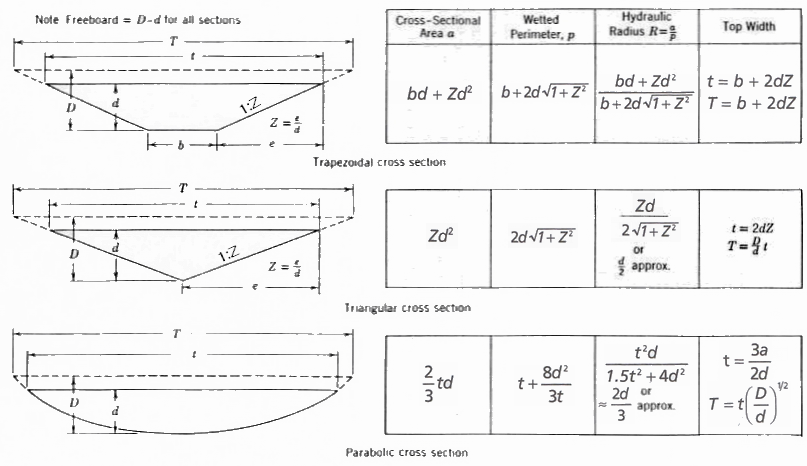
\includegraphics[width=\textwidth]{./img/tvarykoryt}
  \caption{Tvary příčných průřezů úseků hydrografické sítě a použité vztahy na výpočet hydraulického poloměru}
  \label{fig:tvary_koryt}
\end{figure}


\begin{sidewaystable}
% 
% \begin{table}[]
\centering
\caption{Parametry typů půd a kritické hodnoty třecího napětí a nevymílací rychlosti. Kompilát z několika zdrojů, především \cite{DyrovaE.1984, Neumann15:232823}.}
\label{tab:kriticke}
{\small 
\begin{tabular}{lllllllll}
\hline \hline
Název           & ID       & k         & s             & b      & x       & y      & v     & tau   \\
                &          & {[}m/s{]} & {[}m.s-0.5{]} &        &         &        & m/s   & Pa    \\
\hline 
coarse          & CC   & 6.940E-06 & 9.746E-05 & 1.817E+00 & 8.813E+00 & 3.661E-01 & 1.066E+01 & 2.450E-01 \\
medium          & ME   & 1.390E-06 & 1.291E-04 & 1.739E+00 & 1.008E+01 & 5.613E-01 & 1.079E+01 & 2.480E-01 \\
medium fine     & MF   & 2.640E-07 & 1.162E-04 & 1.793E+00 & 9.204E+00 & 4.622E-01 & 1.066E+01 & 2.450E-01 \\
fine            & FF   & 2.780E-06 & 4.746E-05 & 1.703E+00 & 1.067E+01 & 6.028E-01 & 1.150E+01 & 2.640E-01 \\
very fine       & VF   & 1.670E-06 & 1.291E-04 & 1.667E+00 & 1.126E+01 & 6.358E-01 & 1.327E+01 & 3.050E-01 \\
sand            & SS   & 1.000E-06 & 1.291E-04 & 1.817E+00 & 8.813E+00 & 3.661E-01 & 1.066E+01 & 2.450E-01 \\
loamy sand      & LS   & 1.000E-06 & 1.291E-04 & 1.817E+00 & 8.813E+00 & 3.661E-01 & 1.066E+01 & 2.450E-01 \\
sandy loam      & SL   & 5.140E-06 & 9.746E-05 & 1.793E+00 & 9.204E+00 & 4.622E-01 & 1.066E+01 & 2.450E-01 \\
loam            & LL   & 1.670E-06 & 1.291E-04 & 1.739E+00 & 1.008E+01 & 5.613E-01 & 1.079E+01 & 2.480E-01 \\
silt loam       & SIL  & 1.390E-07 & 1.033E-04 & 1.739E+00 & 1.008E+01 & 5.613E-01 & 1.079E+01 & 2.480E-01 \\
silt            & SI   & 1.670E-07 & 1.033E-04 & 1.739E+00 & 1.008E+01 & 5.613E-01 & 1.079E+01 & 2.480E-01 \\
sandy clay loam & SCL  & 5.140E-06 & 9.746E-05 & 1.703E+00 & 1.067E+01 & 6.028E-01 & 1.150E+01 & 2.640E-01 \\
clay loam       & CL   & 1.940E-06 & 4.746E-05 & 1.703E+00 & 1.067E+01 & 6.028E-01 & 1.150E+01 & 2.640E-01 \\
silty clay loam & SICL & 1.670E-07 & 1.033E-04 & 1.703E+00 & 1.067E+01 & 6.028E-01 & 1.150E+01 & 2.640E-01 \\
sandy clay      & SC   & 5.140E-06 & 9.746E-05 & 1.667E+00 & 1.126E+01 & 6.358E-01 & 1.327E+01 & 3.050E-01 \\
silty clay      & SIC  & 1.940E-06 & 4.746E-05 & 1.667E+00 & 1.126E+01 & 6.358E-01 & 1.327E+01 & 3.050E-01 \\
clay            & CC   & 1.940E-06 & 4.746E-05 & 1.667E+00 & 1.126E+01 & 6.358E-01 & 1.327E+01 & 3.050E-01 \\
nosoil          & NO   & 0.000E+00 & 0.000E+00 & 1.585E+00 & 7.985E+00 & 4.889E-01 & 1.000E+02 & 3.000E+00 \\
hlinitá         & HH   & 1.670E-06 & 1.291E-04 & 1.739E+00 & 1.008E+01 & 5.613E-01 & 1.079E+01 & 2.480E-01 \\
hlinitopísčitá  & HP   & 3.670E-06 & 7.746E-05 & 1.793E+00 & 9.204E+00 & 4.622E-01 & 1.066E+01 & 2.450E-01 \\
jíl             & J0   & 1.660E-07 & 1.033E-04 & 1.619E+00 & 1.204E+01 & 6.717E-01 & 1.327E+01 & 3.050E-01 \\
jílovitá        & JJ   & 1.660E-07 & 1.033E-04 & 1.667E+00 & 1.126E+01 & 6.358E-01 & 1.327E+01 & 3.050E-01 \\
jílovitohlinitá & JH   & 2.500E-07 & 1.162E-04 & 1.703E+00 & 1.067E+01 & 6.028E-01 & 1.150E+01 & 2.640E-01 \\
písčitohlinitá  & PH   & 1.670E-06 & 1.291E-04 & 1.739E+00 & 1.008E+01 & 5.613E-01 & 1.079E+01 & 2.480E-01 \\
písčitá         & PP   & 1.670E-05 & 1.936E-04 & 1.817E+00 & 8.813E+00 & 3.661E-01 & 1.066E+01 & 2.450E-01 \\
\hline \hline
\end{tabular}
}
% \end{table}
\end{sidewaystable}



\begin{figure}[t!]
  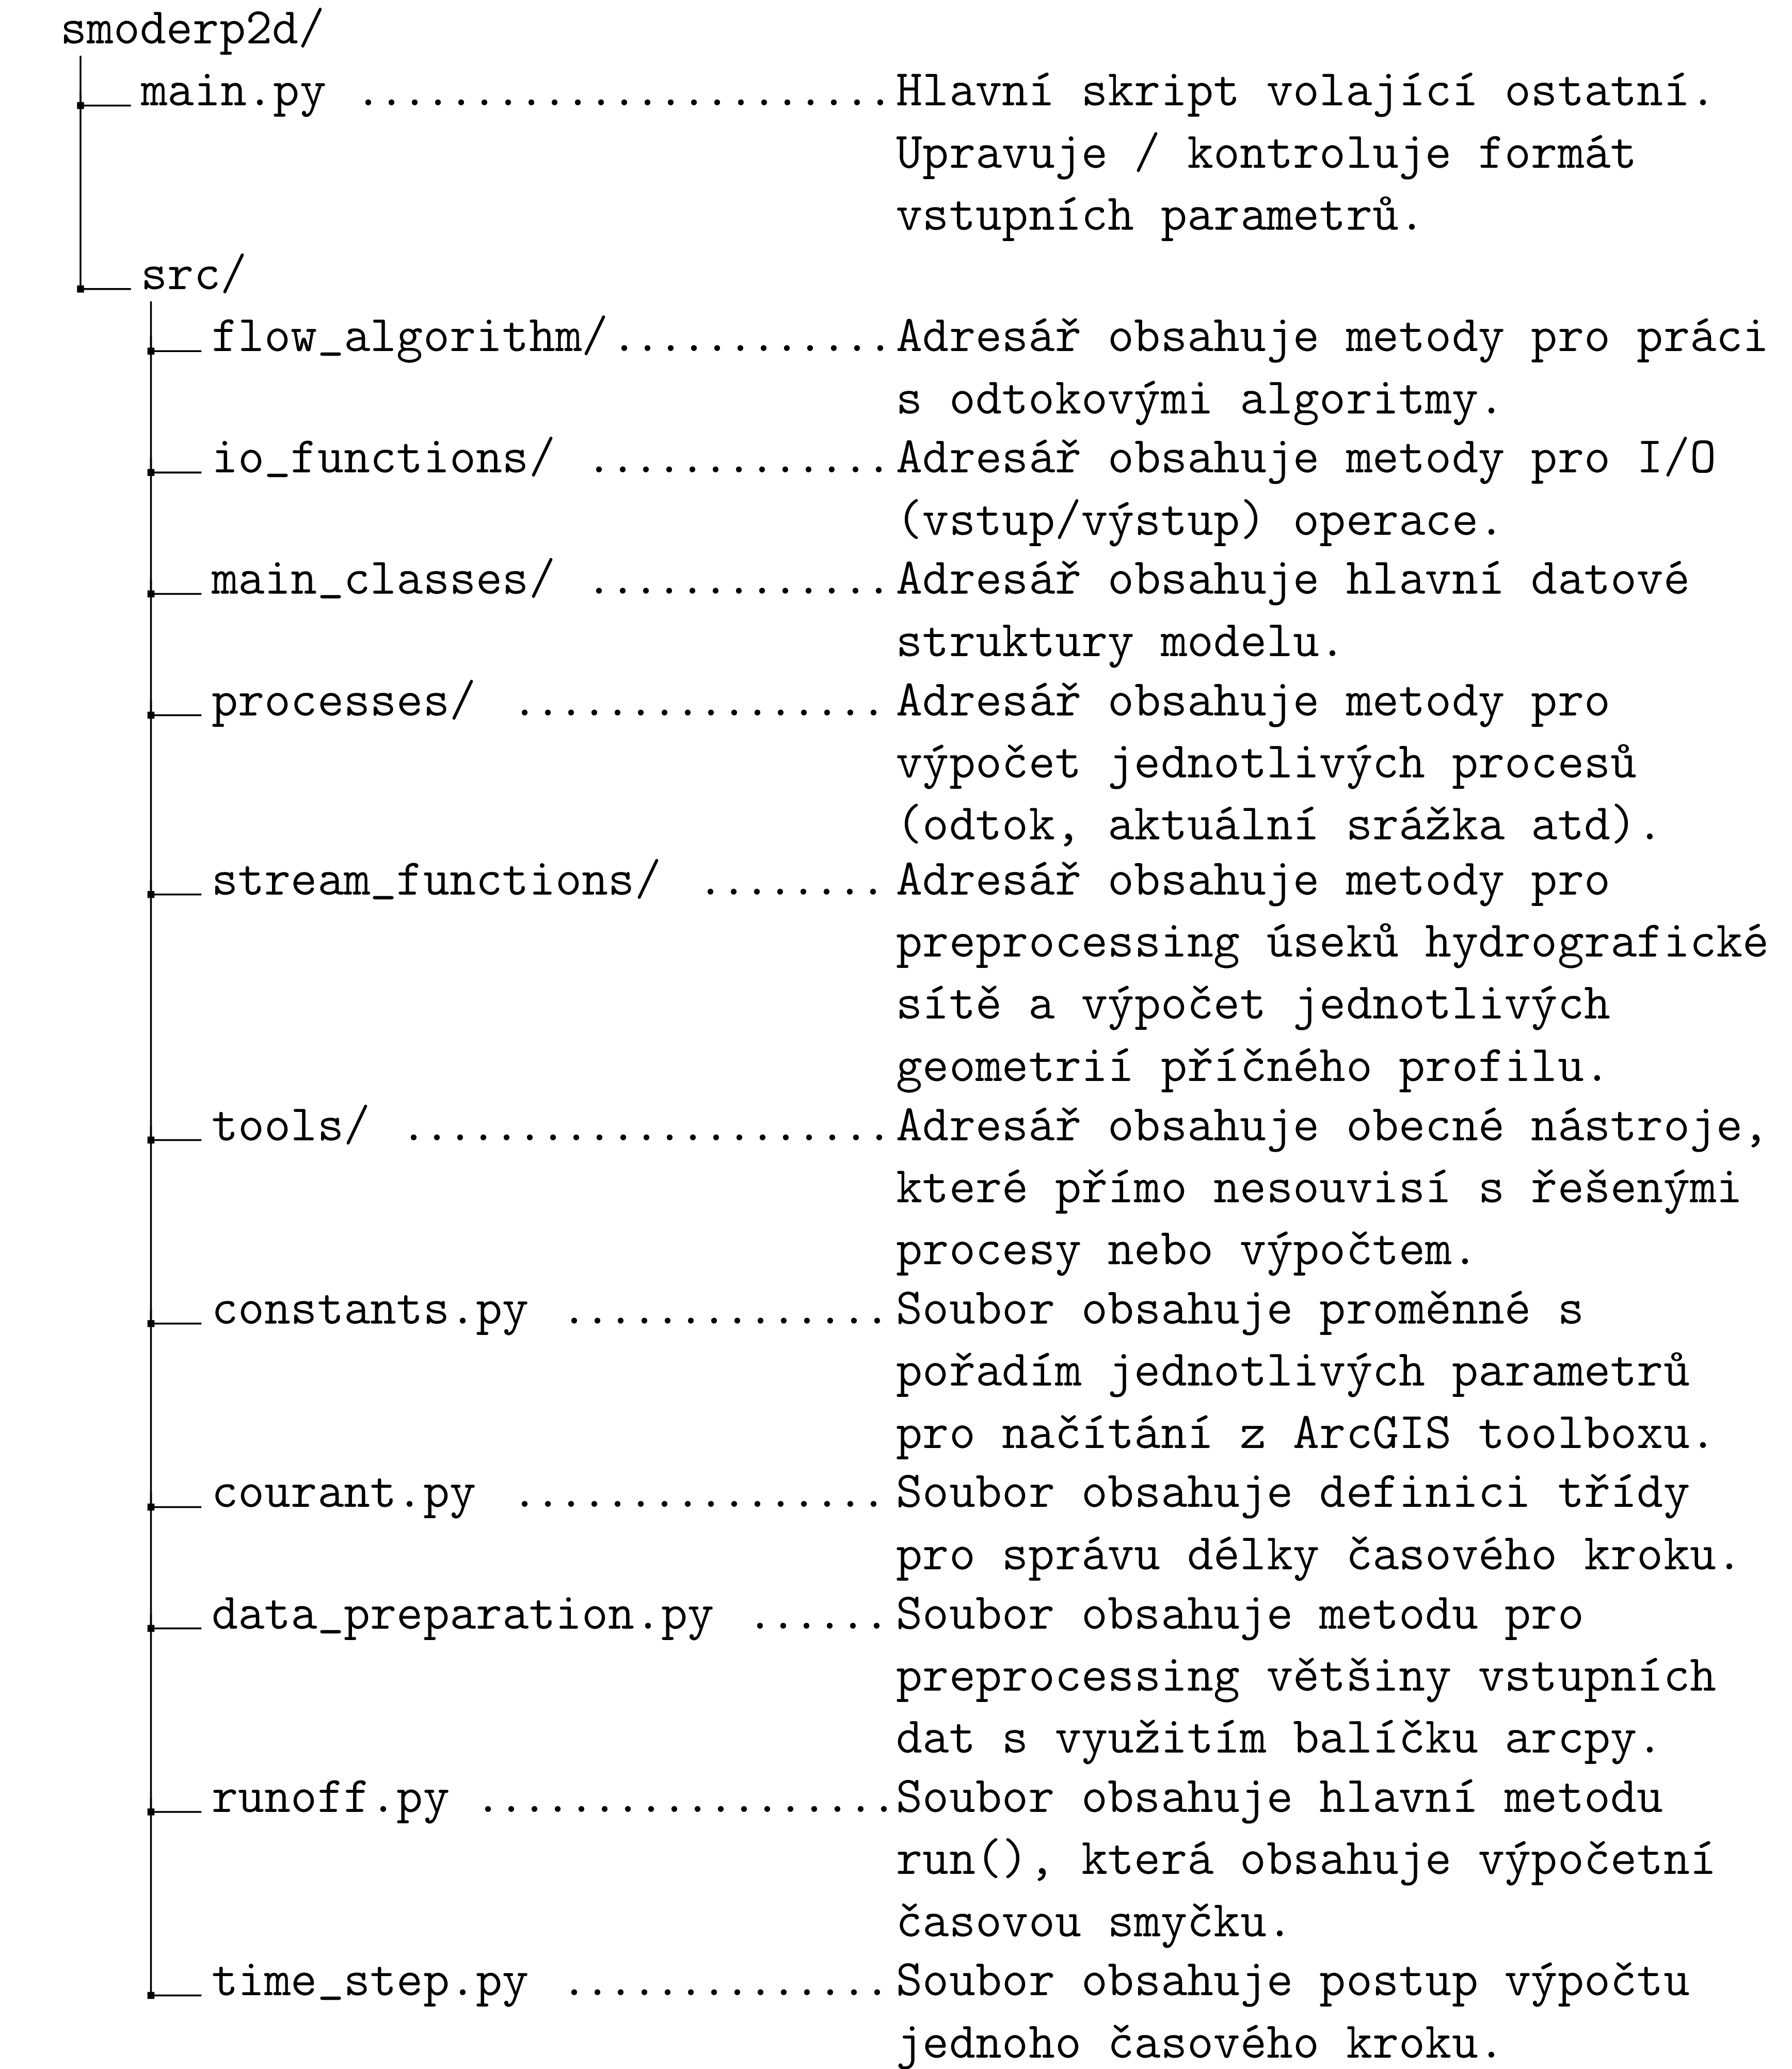
\includegraphics[width=0.8\textwidth]{./img/dirtreenapng.png}
  \caption{důležité soubory a adresáře modelu \smod}
  \label{fig:adresare}
\end{figure}





\begin{figure}[t!]
{\small
\begin{center}
\begin{tikzpicture}[node distance=1.5cm]


\node (start) [startstop] {Start};
\node (dataprep) [process, below of=start] {Příprava dat};
\node (in) [io, left of=dataprep, xshift=-4.0cm] {Vstupní data};

\node (dec1) [decision, below of=dataprep, yshift=-0.5cm] {Konečný čas?};

\node (atm) [process, below of=dec1, yshift=-0.5cm] {Srážka za \acs{dT}};
\node (flow) [process, below of=atm] {Plošný odtok};


\node (check) [process, right of=flow, xshift=2.0cm] {Kontrola \acs{dT}};
\node (updatet) [process, right of=atm, xshift=2.0cm] {Aktualizace \acs{dT}};

\node (dec2) [decision, below of=flow, yshift=-0.5cm] {{\footnotesize Překročení kritické výšky hladiny?}};
\node (rillflow) [process, below of=dec2, yshift=-0.5cm] {Rýhový odtok};

\node (dec3) [decision, below of=rillflow, yshift=-0.5cm] {Je buňka v toku?};
\node (streamflow) [process, below of=dec3, yshift=-0.5cm] {Odtok úsekem toku};

\node (output) [io, below of=streamflow, yshift=-0.5cm] {Výstupní data};
\node (stop) [startstop, below of=output, yshift=-0.5cm] {Konec};

% uzly ohnutym caram
\node (dd1) [guide, right of=rillflow, xshift=2.0cm] {};
\node (dd2) [guide, right of=dec1, xshift=2.0cm] {};
\node (dd3) [guide, right of=dec2, xshift=2.0cm] {};
\node (dd4) [guide, right of=dec3, xshift=2.0cm] {};
\node (dd5) [guide, right of=streamflow, xshift=2.0cm] {};
\node (dd6) [guide, left  of=dec1, xshift=-2.0cm] {};
\node (dd7) [guide, left  of=output, xshift=-2.0cm] {};


% jednotlive sipky
\draw [arrow] (start) -- (dataprep);
\draw [arrow] (in) -- (dataprep);
\draw [arrow] (dataprep) -- (dec1);
\draw [arrow] (dec1) -- node[anchor=west] {ne} (atm);
\draw [arrow] (atm) -- (flow);
\draw [arrow] (flow) -- (dec2);
\draw [arrow] (dec2) -- node[anchor=west] {ano} (rillflow);
% \draw [arrow] (dec1) -- node[anchor=north] {ano} (output);
\draw [arrow] (output) -- (stop);
\draw [arrow] (rillflow) -- (dec3);
\draw [arrow] (dec3) -- node[anchor=west] {ano} (streamflow);
\draw [arrow] (check) -- (updatet);


% ohnute cary line (jen cara) do guide (jen neviditelny bod)
%             arrow  z guide (jen neviditelny bod) tam kam chci

\draw [line] (updatet) -- (dd2);
\draw [arrow] (dd2) -- (dec1);

\draw [line] (dec2) -- node[anchor=north] {ne}(dd3);
\draw [arrow] (dd3) -- (check);

\draw [line] (dec3) -- node[anchor=north] {ne}(dd4);
\draw [arrow] (dd4) -- (check);

\draw [line] (streamflow) -- node[anchor=north] {}(dd5);
\draw [arrow] (dd5) -- (check);


\draw [line] (dec1) -- node[anchor=north] {ano}(dd6);
\draw [line] (dd6) -- (dd7);
\draw [arrow] (dd7) -- (output);



\end{tikzpicture}
\end{center}
}
\caption{Flow chart toku programu}
\label{fig:flowchart}
\end{figure}





  \newpage

  \part*{Seznam použitých zdrojů}
  \bibliographystyle{agsm}
  \bibliography{bib/bib}


\end{document}


